\documentclass[12pt]{book}
\usepackage[a5paper]{geometry}

\usepackage[utf8]{inputenc}
\usepackage[T1]{fontenc}
% \usepackage[russian]{babel}
\usepackage{tipa}
% \usepackage[german]{babel}
\usepackage{graphicx}

\setlength{\parindent}{1em}
%\setlength{\parskip}{1em}

\DeclareUnicodeCharacter{0166}{\barredT}
\DeclareUnicodeCharacter{0167}{\barredt}

\DeclareRobustCommand{\barredT}{\barredTt{0.5}{0.05}{1.5}{T}}
\DeclareRobustCommand{\barredt}{\barredTt{0.4}{0}{1.15}{t}}
\newcommand{\reducedhyphen}[2]{%
	\raisebox{#1ex}{\scalebox{#2}[0.5]{-}}%
}
\newcommand{\barredTt}[4]{%
	\begingroup
	\vphantom{#4}%
	\ooalign{%
		#4\cr
		\hidewidth\kern#2em\reducedhyphen{#1}{#3}\hidewidth\cr
	}%
	\endgroup
}

\begin{document}
\begin{titlepage}

\author{Krizhanich Research Institute of Novoslovnica}
\title{%
	Novoslovnica \\
	\large Guide through a Slavic constructed language
\vfill
}
\date{2015-2019}

\end{titlepage}

\frontmatter
\maketitle
\tableofcontents
\mainmatter
\chapter{Phonology}

Every language has its own phonology. But do you know what phonology is?

Phonology - a branch of linguistics concerned with the systematic organization of sounds in the language.

Thus, phonology describes all the sounds that the language possesses. Sounds can be divided into different classes. One of the characteristics separating different sounds is the ability to pronounce them with an open vocal tract. You can notice that vowels (such as a, o, u in English) are able to be pronounced with open vocal tract, whereas consonants are pronounced with partly or completely closed vocal tract. So, let's discuss the sounds from the point of this classification.

However, firstly we should speak about the term allophone.

Allophone - one of a set of multiple possible spoken sounds or signs used to pronounce a single phoneme in a particular language.

Well, what is a phoneme? A phoneme is one of the units of sound that distinguish one word from another in a particular language. Simply put, it is such a sound (or a set of sounds) that do not influence the meaning of the word. 


\section{Vowels}

In the beginning of this paragraph I would like to write a description of a vowel.

Vowel - a sound produced with no constriction in the vocal tract.

With this information we can distinguish different types of vowels. The classification of vowels is based on two main factors:
What is the row of the sound
What is the height of the sound
Whether the vowel is rounded or not

The row is the position of the tongue when you pronounce a vowel. There are three main rows: front, central and back. When you pronounce a vowel at the front row, you move your tongue toward the teeth. The descriptions of central and back rows are similar - you move your tongue to the center or toward the larynx to pronounce them.

The height of the sound is a characteristic of tongue convexity and tension in your mouth. If it is positive, it means your tongue does not touches the palate nor bottom of the mouth, and the tip of your tongue is tense- or closed. If your tongue is flat and parallel to the bottom of your oral cavity, moreover, it lies on it - it is an open one. Between these two positions a middle position can be found.

The roundedness of the vowel is the amount of rounding in the lips during the articulation of a vowel. Vowels can be categorized as rounded and unrounded. Thus, to pronounce a rounded vowel you should round your lips. To pronounce an unrounded vowel, you should relax your lips during the articulation of a vowel.

Finally, we can talk about Novoslovnica phonology. Novoslovnica consists of 20 ordinary vowel phonemes. Among them there are seven closed vowels, three open vowels, ten middle vowels as well as seven front vowels, five center vowels and eight back vowels. On the table 1.1 you can see a chart position of the vowels in Novoslovnica.

\begin{table}[]
	\begin{tabular}{lllll}
		& Front & Center & Near-back & Back \\
		Close      &       &        &           &      \\
		Near-close &       &        &           &      \\
		Close-mid  &       &        &           &      \\
		Mid        &       &        &           &      \\
		Open-mid   &       &        &           &      \\
		Open       &       &        &           &     
	\end{tabular}
\end{table}

In this table you can also see different colors of the vowels. The green ones are for rounded vowels. Yellow ones are for unrounded vowels.

If you know Czech or Finnish, you might be concerned by the absence long vowels in this chart. It’s time to speak about allophones in Novoslovnica.

Novoslovnica has allophones of open and long vowels. This means that it does not matter how you pronounce a “modified” vowel - as a long one or as an open one - the meaning of the word will not change. To make this more clear, look at table 1.2.


\chapter{Orthography}

\begin{figure}
	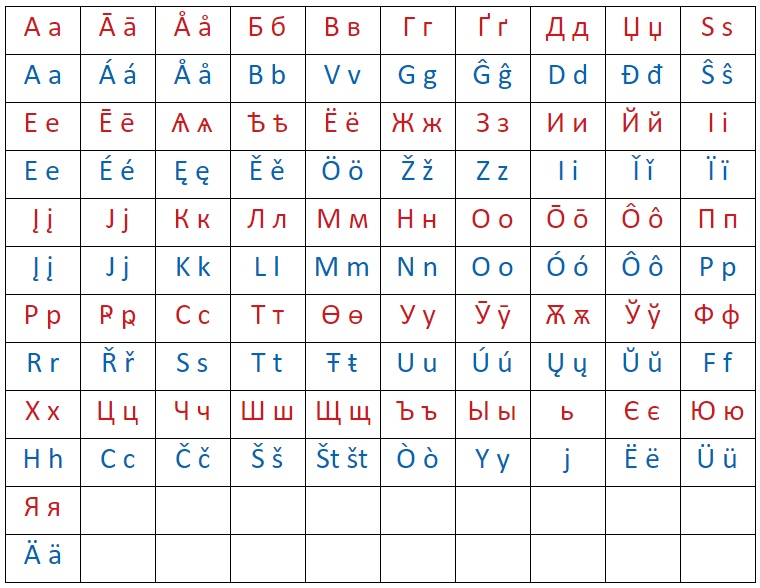
\includegraphics[width=\linewidth]{./sources/alphabet.jpg}
	\caption{Alphabet of Novoslovnica}
	\label{fig:alphabet}
\end{figure}

\section{Alphabet}

Let’s summarize what we have known about Novoslovnica phonology. Afterwards we will get the list of phonemes and allophones and their connections with Novoslovnica letters in the alphabet.

We have learned that Novoslovnica has 51 consonant sounds and 22 vowels. 13 consonants and 4 vowels are allophones among them. Hence, the amount of phonemes is (51-13) + (22 - 4) = 56 phonemes.

You should know that in Novoslovnica, soft and hard consonants do not differ in writing. That is because of the fact that by the combination of “consonant + vowel” we can always determinedly get what the consonant is like - hard or soft. With this information, the amount of letters needed is reduced to 49 \cite{nsl-alphabet}.

Nevertheless, let’s now look at the table with the alphabet list and see how Novoslovnica is written.

% \begin{table}
	\begin{longtable}{llllp{4em}p{6em}}
		No. & Char & Cyr & Phoneme & Allophone & Examples in English \\
		\endhead
		1 & A a & А а & \textipa{[a]} & & Ex\textbf{a}mple, p\textbf{a}st (British forms) \\
		2 & Ä ä & Я я & \textipa{[\ae]} &  & Cat, rat (American English) \\
		3 & Á á & Ā ā & \textipa{[a:]} & \textipa{[A]} & M\textbf{a}rk, p\textbf{a}rk \\
		4 & Å å & Å å & \textipa{[2]} & & C\textbf{u}t, w\textbf{o}nder \\
		5 & B b & Б б & \textipa{[b]} & \textipa{[bj]} & \textbf{B}etter, \textbf{b}ear \\
		6 & C c & Ц ц & \textipa{[\t{ts}]} & \textipa{[\t{ts}j]} & Tea, team (In some American or British dialects) \\
		7 & Č č & Ч ч & \textipa{[\t{tS}]} & \textipa{[\t{tC}], [\t{t\:s}]} & Cheese, check \\
		8 & D d & Д д & \textipa{[d]} & \textipa{[\textbardotlessj]} & Do, dinner \\
		9 & Đ đ & Џ, џ & \textipa{[\t{\:d\:z}]} & \textipa{[\t{d\textctz}], [\t{dZ}]} & John, June \\
		10 & E e & Е е & \textipa{[E]} & & Pet, set \\
		11 & Ë ë & Є є & \textipa{[\|`e]} & & \\
		12 & É é & Ē ē & \textipa{[E:]} & \textipa{[3]} & \\
		13 & Ě ě & Ѣ ѣ & \textipa{[e]} & \textipa{[I]} & \\
		14 & Ę ę & \cyrsyus & \textipa{[\~E]} & \textipa{[eN]} & \\
		15 & F f & Ф ф & \textipa{[f]} & \textipa{[fj], [\r*U], [\r*Uj]} & Feather, phone \\
		16 & G g & Г г & \textipa{[H]} & \textipa{[G], [Gj], [Hj]} & Horn, behind (Australian English) \\
		17 & Ĝ đ & \CYRGUP \cyrgup & \textipa{[g]} & \textipa{[gj]} & Go, grow \\
		18 & H h & Х х & \textipa{[x]} & \textipa{[xj], [h], [hj]} & Hair, horror \\
		19 & I i & И и & \textipa{[I]} & & Kitten, rid \\
		20 & Ï ï & I i & \textipa{[i]} & & Meet, seat \\
		21 & Ǐ ǐ & Й й & \textipa{[j]}  & & My, tie (the last part of the diphthong) \\
		22 & Į į & Į į (\cyryn) & \textipa{[\~E]} & \textipa{[iN]} & Evening, morning \\
		23 & J j & J j (ь)& \textipa{[J]} & & Yogurt, yard \\
		24 & K k & К к & \textipa{[k]} & & Calm. pocket \\
		25 & L l & Л л & \textipa{[l]} & & Lemon, climate \\
		26 & M m & М м & \textipa{[m]} & & Month, memory \\
		27 & N n & Н н & \textipa{[n]} & & Noun, coin \\
		28 & O o & О о & \textipa{[o]} & & Cotton \\
		29 & Ö ö & Ё ё & \textipa{[8]} & & Bird, sir \\
		30 & Ó ó & Ō ō & \textipa{[o:]} & & Pole \\
		31 & Ò ò & Ъ ъ & \textipa{[@]} & & \\
		32 & Ô ô & Ô ô & \textipa{[\|`o]} & & Pool, good \\
		33 & P p & П п & \textipa{[p]} & & Pear, sweep \\
		34 & R r & Р р & \textipa{[r]} & & Race, parent \\
		35 & Ř ř & \cyrrz & \textipa{[\r*r]} & & \\
		36 & S s & С с & \textipa{[s]} & & Press, costume \\
		37 & Š š & Ш ш & \textipa{[\v{s}]} && Shine, mushroom \\
		38 & Ŝ ŝ & Ѕ ѕ & \textipa{[\t{dz}]} & & Day, dime (In some American or British dialects)  \\
		39 & T t & Т т & \textipa{[t]} & & Todd, torture \\
		40 & Ŧ ŧ & \CYROTLD   \cyrotld & \textipa{[T]} & & Throne, health \\
		41 & U u & У у & \textipa{[u]} & & Put, \\
		42 & Ü ü & Ю ю & \textipa{[0]} & & Pure, cute \\
		43 & Ú ú & Ӯ ӯ & \textipa{[u:]} & & Poor \\
		44 & Ŭ ŭ & Ў ў & \textipa{[w]} & & Wonder, way \\
		45 & Ų ų & Ѫ ѫ & \textipa{[uN]} & & \\
		46 & V v & В в & \textipa{[v]} &\textipa{[vj], [V], [Vj]} & \textbf{V}al\textbf{v}e, \textbf{v}el\textbf{v}et \\
		47 & Y y & Ы ы & \textipa{[1]} & & \\
		48 & Z z & З з & \textipa{[z]} & & Zone, zoo \\
		49 & Ž ž & Ж ж & \textipa{[\:z]} & & Closure, measure \\
	\end{longtable}
% \end{table}

Note, that the Cyrillic letters Щ, $\Psi$, Ќ, Ї in earlier versions of Novoslovnica have been replaced by Шт (Št), Пс (Ps), Кс (Ks) and Ји (Jі).\footnote{Cyrillic has two different letters \textit{Ь} and \textit{J} that have different functions - the first one defines that the previous consonant is soft (we need this in case vowel is absent) and the second defines a [\textctj] sound. Latin version that you see in the table has no such difference, so you should remember, that J means a soft symbol when you see a C-”J”-C row (where C is for “Consonant”) and means a [\textctj] sound when you see a C-”J”-V (where V is for “Vowel”), or use Cyrillic to prevent such a collision. Only in the first case consonant before J is soft while in the second one it is hard.}
% надо добавить, что в югославянских Ь, Й и Ј слились в Ј (в полесском только Й замещена Ј), что, впрочем имело параллекли и в глаголице (как болгарской, так и хорватской), где кроме отдельной буквы для Ь был значок "штапик/штапић" который соответствовал и Ь и Ј.

\section{Pronunciation}

Novoslovnica is a phonetic language, that’s why Novoslovnica has an important rule, which you have to apply to speaking in Novoslovnica.

\textbf{Rule n. 3}: All words are pronounced as they are written.

This rule means that you cannot reduce sounds when speak in Novoslovnica. It is a very important thing because you can make mistakes if you speak improperly. There are some exceptions but they all will be mentioned in this guidebook.

When you pronounce a word you are not restricted to use only main sounds - if it’s more comfortable, you can pronounce allophones with the same level of softness and sonority with the main sound of the letter. Let’s look at the examples below to understand what we can choose in speaking and what we cannot.

\textbf{Examples:}

jsdasd

asdasd

However, you are restricted in what consonant sounds to use from the allophone list. You can see the next rule which will help you to speak.

\textbf{Rule n. 4}: You cannot mess soft and hard consonants when you pronounce a word.

This prohibit you to make hard consonants when you need a soft one, or to use a soft one when you need a hard one. Here you can see a table, where it is shown which sound you must pronounce in different combinations of letters.

\begin{longtable}{lllll}
%	\begin{tabular}{lllll}
		Letter & Next letter & IPA & Examples & Translations \\
		\endhead
		b & a o e i u y ų  & [b] && \\
		b & ä ö ë ï ü & [bj] && \\
		v & a o e i u y ų & [v] && \\
		v & ä ö ë ï ü & [vj] && \\
		g & a o e i u y ų & \textipa{[H]} && \\
		g & ä ö ë ï ü & \textipa{[Hj]} && \\
		ĝ & a o e i u y ų  & [g] && \\
		ĝ & ä ö ë ï ü & [gj] && \\
		d & a o e i u y ų & [d] && \\
		d & ä ö ë ï ü & \textipa{[\textbardotlessj]} && \\	
		đ & a o e i u y ų & \textipa{[\t{\:d\:z}]} & & \\
		đ & ä ö ë ï ü & \textipa{[\t{dZ}]} && \\
		ŝ & a o e i u y ų  & \textipa{[\t{dz}]} && \\
		ŝ & ä ö ë ï ü & \textipa{[\t{dzj}]} && \\
		k & a o e i u y ų & [k] && \\  
		k & ä ö ë ï ü  & [kj] && \\ 
		l & a o e i u y ų  & [l] && \\  
		l & ä ö ë ï ü  & \textipa{[L]} && \\ 
		m & a o e i u y ų  & [m] && \\  
		m & ä ö ë ï ü  & [mj] && \\
		n & a o e i u y ų  & [n] && \\  
		n & ä ö ë ï ü  & \textipa{[\textltailn]} && \\
		p & a o e i u y ų & [p] && \\  
		p & ä ö ë ï ü  & [pj] && \\ 
		r & a o e i u y ų  & [r] && \\  
		r & ä ö ë ï ü  & [rj] && \\
		ř & a o e i u y ų  & \textipa{[\r*r]} && \\  
		ř & ä ö ë ï ü  & \textipa{[\r*rj]} && \\ 
		s & a o e i u y ų & [s] && \\  
		s & ä ö ë ï ü  & [sj] && \\ 
		t & a o e i u y ų  & [t] && \\ 
		t & ä ö ë ï ü  & [c] && \\ 
		ŧ & a o e i u y ų  & \textipa{[T]} && \\  
		ŧ & ä ö ë ï ü  & \textipa{[Tj]} && \\ 
		f & a o e i u y ų  & [f] && \\  
		f & ä ö ë ï ü  & [fj] && \\
		h & a o e i u y ų   & [h] && \\
		h & ä ö ë ï ü  & [hj] && \\
		c & a o e i u y ų   & \textipa{[\t{ts}]}&& \\
		c & ä ö ë ï ü  & \textipa{[\t{tsj}]} && \\
		č & a o e i u y ų   & \textipa{[\t{tS}]} && \\
		č & ä ö ë ï ü  & \textipa{[\t{tSj}]} && \\
		š & a o e i u y ų   & \textipa{[\v{s}]} && \\
		š & ä ö ë ï ü  & \textipa{[\v{s}j]} && \\		
%	\end{tabular}
\end{longtable}

\section{Some features}

I and Ï

Many people will surely be confused by these two letters. They will ask whether there is the rule when we need to write the first ot the second one. However, you should look up and remember that these both letters produce different sounds. And that is the point. 

The first letter produces the soft sound “I” while the second one stands for the hard sound. But the question is, where are used such sounds? We can't list the rules for usage these letters in the root, because it is etymological issue. However, we can list some prefixes and suffixes that contain the soft or the hard letter.

Marks for writing “I”:

Prefixes 

- Iz

Suffixes

- Nic

- Nik

- Itelj

- I

Conjunction

- I

- Ili

- Či

- Li

Marks for writing “Ï”:

Prefixes

- Nïz

Suffixes

- Ïc (female animals)

\section{Latin and Cyrillic}

You can see in table 1.8 that Novoslovnica utilizes two alphabets- the Latin one and the Cyrillic one. They both are practically equal, but is there is a preferred alphabet for the language? The answer is “yes”, Cyrillic is preferable.

The reasons of choosing such a script goes back in history. There were two scripts in the beginning of Slavic writing: the Glagolitic and Cyrillic scripts. They were created to cover all the sounds that existed in that era of Slavic languages. Glagolitic script practically has no borrowed letters from other writing systems- all letters are unique.

By this case in Cyrillic and Glagolitic scripts we can find the bijective mapping between sounds (phonemes) and letters. Latin script does not provide such orthography in any Slavic language which uses the Latin script. 

For \textbf{example}:

- “ch” for [x], while “c” is for [\textipa{\t{ts}}] and h is for [\textipa{H}]

- “sz” for [\textipa{\:s}], while “s” is for [s] and “z” is for [z]

Novoslovnica provides an artificial Latin script system, where the bijective mapping has almost been achieved. The Latin alphabet can seem strange or uncomfortable to native Slavs \footnote{Latin script is very habitual for South Slavs and native for West Slavs} (though it can be used rather conveniently by non-Slavs). That’s why the Glagolitic or Cyrillic script should be used primarily.

Why hasn’t the Glagolitic script been mentioned yet? The same reason that the Latin script should not be used primarily: to prevent misunderstanding. Nowadays only one in a hundred Slavs can understand the Glagolitic script because all of its letters are original. That’s why this language, which has the goal of being used on the international level, cannot use Glagolitic script as its primary script.

The only script, that satisfies all the requirements to be the primary script of this Slavic constructed language, is the Cyrillic alphabet. In this book you will find many examples in different paragraphs. First you will see a primary (Cyrillic) variant of the example in normal font and then a Latin one in grey italic font. This will help you to learn primary script of Novoslovnica quickly. Nevertheless, if we speak about exact letters or letter combinations, I will write them only in Latin for not to mess the text of the book.

Now you know the sounds and the letters which are used in Novoslovnica and you are ready to go deeper!

\chapter{Grammar}

Grammar\index{grammar} is the core of every language. Grammar comprises different themes that are united in a system of changing words enough for building sensible syntax constructions. We will look at Novoslovnica grammar from the point of parts of speech.

\newglossaryentry{pos}{name=POS, description={Part of speech}}

\textit{Part of speech\index{part of speech} (\gls{pos})} - is a category of words which have similar grammatical properties.

Thus, we unite a group of words into parts of speech when they have a lot of similar grammar properties such as “number”, “person”, “case”, “tense” etc. In this chapter we will go through different parts of speech and study what differences they have and how we should identify each of them and combine them to be able to create phrases and sentences. 

Parts of speech comprise two main categories - independent\index{independent POS} POS and auxiliary\index{auxiliary POS} POS. The fact the POS is independent or not refers to its semantic values. An independent POS has a full semantic value that can be used separately.  That means when you say a word of an independent POS you reproduce some semantic meaning that the interlocutor can recognize. An auxiliary POS has a meaning that a partial semantics that is partially defined and can be distinguished only in pair with a word of an independent POS.

\textbf{Example:}

\textit{River} - this word can be recognized by interlocutor as some concept of water flowing in a restricted area.

\textit{Beautiful} - this word is recognized as an attribute of any concept that is nice, pleasant to the person (i.e. speaker or interlocutor)

\textit{Came} - this word can be recognized as any concept’s action of going to the destination point and having reached it. 

And so on. Nouns, adjectives, verbs, adverbs, participles, numerals, pronouns refer to independent POS. You see that every word has its own meaning enough full to imagine yourself some information you have been received. This is not true for a word of an auxiliary POS. 

\textit{On} - this word can be recognized as a placement of an object against some horizontal surface. It can refer to some time moment (be on time). It can also be used with a fully different value (come on - to increase the activity of doing something).

\textit{For} - it can be recognized as an aim for something or an object with participates in some action. Also this word can refer to a duration of a process.

Moreover, words “and” or “to” cannot give you any map in your mind into any sensible meanings. Though these words have no determined semantic value, they are extremely important in the whole phrase connecting two words of the same POS with logical value (AND, OR, NOT). English language is an analytical one, that is why words are mostly connected with each other in the phrase by an auxiliary POS. Without them you are not able to understand what the person is speaking about. Slavic languages are fusional, however, there are enough analytic features in them, hence auxiliary parts of speech are also important. Articles, prepositions and conjunctions are referred to auxiliary parts of speech.

There are also two additional categories - particles and interjections. Some allocate them into separate categories, some claim they belong to an auxiliary category. Nevertheless, these are both separated parts of speech because they have different grammar properties.

Particles added to words are close to some additional functions. If you delete them from your phrase, there will be no change in the whole meaning (that is why one cannot say they are of an auxiliary POS), but with presence of particles you will get more additional semantic or sometimes emotional information named \textit{color}. English language has very few particles. The most known is “to” as an infinitive indicator particle of a verb. Controversially, Slavic languages have a bit more particles that are rather popular in the spoken language. They form several groups by their semantic color.

\textbf{Examples:}

\textit{Ja sòm govoril tobě.} - I have told you.

\textit{Ja sòm govoril že tobě!} - I have told you!

Additional semantic meaning. The speaker shifts emphasis from undefined (neutral phrase) to the word “govoril” (told). So the interlocutor now has a determined emphasis of the phrase. The speaker wants to say that he has already told the same fact to the interlocutor and he was right because something happened confirming them.

Interjection is a POS that have no semantic meanings. They are not words in our common comprehension. Interjections are sounds that we produce. It is rather difficult to say sometimes what differences are between interjections and senseless sounds that we can produce (i.e. some spontaneous exclaims, murmuring etc.). Interjections are divided into intended exclaims (with bright emotional color) and sound imitations (i.e. animal voices imitation) that are united in the group of Onomatopoetics.

These are all categories of POS. If we speak about an independent POS, we should take into account that there are different semantic, morphological and syntax functions can be described by it. There several type of semantic functions: the concept, the attribute, the predicate and the demonstrative.

The \textit{concept} is something that correlates with the object or subject in the real world. It could be either abstract or imaginary, but we can ask a questions “Who? What?” about it.

The \textit{predicate} is something that determines the action, corresponding to a concept. We often ask questions “What to do?” to reveal a predicate.

The \textit{attribute} is something that is correspond to a concept or an action. We ask questions “What concept is like?” or “What action is like?” to find out the determine value of the attribute.

The \textit{demonstrative} points out the concept. It has the same question with the attribute yet has no semantic value but demonstrating a concept it corresponds with. 

Parts of speech that have properties of a concept are nouns, cardinal numerals, verbal noun and some kinds of pronouns.

Parts of speech that have properties of an attribute are adjectives, participles, ordinal numerals and adverbs.

Parts of speech that have properties of a predicate are verbs, transgressive, and gerund.

Parts of speech that have demonstrative properties are most kinds of pronouns.

Thus, noun, adjective, verb, adverb, numeral, pronoun, gerund and participle are independent, while preposition, particle, interjection (with Onomatopoetic), article and conjunction are auxiliary ones.

Independent parts of speech are also divided into nominal and verbal ones. It is extremely important because this division shows differences in grammar forms of nominal and verbal POS. Verb, participle, transgressive, gerund are verbal parts of speech, while noun, adjective, numeral are nominal. Adverbs and pronouns stay separately - the first one because of its immutability and the second one because of its heterogenity. 

In the chapter it will be spoken about the very POS exists in Novoslovnica. In the beginning of each section the table with grammar and semantic properties of a POS will be given.

First of all you should know some facts about different grammatical properties in Novoslovnica.

\newcounter{casechapter}[section]
\section{Case}

Case\index{case} is a grammatical property of a nominal POS (Part of speech) that shows what references this nominal POS has with other words in a sentence (phrase). This property is widely known in fusional languages, while analytical languages do not often possess this property. Thus, English has only two active cases - Nominative and Oblique one. Moreover, oblique case is used practically only within pronouns while nouns have no such a case. That means case is not the only way to show references between nominal POS and other words in a sentence. Case is just one of the ways to show it and Slavic languages as being fusional widely use this grammar category.

Different Slavic languages have different number of cases. For example, Russian language has six cases while Serbian language has seven. We can find exceptions in Bulgarian and Macedonian languages, which are analytical that is why they have only one case for a noun and adjective and three cases for a pronoun.

Different cases are referred to different semantic links between words. It is the cause why we see ambiguity of cases in different languages (that have different amount of cases and different usage rules of cases). Novoslovnica provides most common and wide means to use cases with almost full determination. When you speak Novoslovnica you have to use the case of exact semantic value and not of the longstanding phraseology of your own language.

With this principle Novoslovnica establishes nine cases. Nine changing patterns that determine alterations of all words of nominal POS. This is the unification of Slavic languages in the sphrere of fusial word linking. Here they are:

\newglossaryentry{nominative}{name=P.C., description={Nominative}}
\newglossaryentry{genitive}{name=G.C., description={Genitive}}
\newglossaryentry{partitive}{name=P.C., description={Partitive}}
\newglossaryentry{accusative}{name=A.C., description={Accusative}}
\newglossaryentry{dative}{name=D.C., description={Dative}}
\newglossaryentry{instrumental}{name=I.C., description={Instrumental}}
\newglossaryentry{prepositional}{name=Pr.C., description={Prepositional}}
\newglossaryentry{locative}{name=L.C., description={Locative}}
\newglossaryentry{vocative}{name=V.C., description={Vocative}}

\begin{itemize}
	\item Nominative (\gls{nominative})
	\item Genitive (\gls{genitive})
	\item Partitive (\gls{partitive})
	\item Dative (\gls{dative})
	\item Accusative (\gls{accusative})
	\item Instrumental (\gls{instrumental})
	\item Prepositional (\gls{prepositional})
	\item Locative (\gls{locative})
	\item Vocative (\gls{vocative})
\end{itemize}

In this chapter we will speak about cases in general. All examples will disclose case features through nouns as examples.

Nominative\index{case!nominative} case (\textit{Imenóvnik}) is used when we are talking about a concept as an actor. If the sentence is full, the subject is in Nominative. You can ask questions like «Who? What?» to it.

This case is basic in most languages, so POSes in this case are supposed to be in the normal form (that we can find in a dictionary). In Novoslovnica nominative also determines a normal from of the word. In the examples you can see full sentenses, where subject is used in nominative.

\textbf{Examples:}

\stepcounter{casechapter}
\arabic{chapter}.\arabic{section}.\arabic{casechapter} \textit{\textbf{Dom}-òt je vëlïkym.} - The \textbf{house} is big.

\stepcounter{casechapter}
\arabic{chapter}.\arabic{section}.\arabic{casechapter} \textit{\textbf{Izučilišto}, de ja sę učam, je starym}. - The \textbf{school} I attend is old.

\stepcounter{casechapter}
\arabic{chapter}.\arabic{section}.\arabic{casechapter} \textit{Klüč-òt je od ovoŭ vråtoŭ.} - The key is to these doors.

Genitive\index{case!genitive} case (\textit{Čyǐnik}) is used when we are talking to an object being related to another one. Thus this case show what generation the object is of and what is it made from or whom does it belong to. The questions that determine the case are «Whose? Which? What?».

In Novoslovnica possessive case equals to genitive one, so English «'s» constructions should be translated in genitive (example 4.1.4). Further, genitive in Novoslovnica could be related to usage of nouns with «of» preposition (example 2, 3).

\textbf{Examples:}

\stepcounter{casechapter}
\arabic{chapter}.\arabic{section}.\arabic{casechapter} \textit{Kniga \textbf{brata} je vëlïmi zajimliva.} — My \textbf{brother}'s book is very fascinating.

\stepcounter{casechapter}
\arabic{chapter}.\arabic{section}.\arabic{casechapter} \textit{Cěna \textbf{uspěha} je mnogo vëlïka.} — The price of \textbf{success} is very high.

\stepcounter{casechapter}
\arabic{chapter}.\arabic{section}.\arabic{casechapter} \textit{Sklad je na koncu \textbf{ulicy}-ta.} — The shop is at the end of the \textbf{street}.

Partitive\index{case!partitive} case (\textit{Ličóvnik}) is used when we are talking about some amount of object having or being supposed to have uncountable properties. The questions that determine the case are «Of what? With what? How much of?».

This case has many coinciding forms with genitive, though in masculine gender it has another endings (examples 1, 3). In English it should be translated with «of» construction (example 1). If uncountable nouns are used with the predicate directly or with adverbs of measure, they should be translated into Oblique case in English (example 2, 3).

\textbf{Examples:}

\stepcounter{casechapter}
\arabic{chapter}.\arabic{section}.\arabic{casechapter} \textit{Daǐ mi čašku \textbf{čaju}.} — Give me a cup of \textbf{tea}.

\stepcounter{casechapter}
\arabic{chapter}.\arabic{section}.\arabic{casechapter} \textit{Dodaǐ do pïroga němnogo \textbf{vody}.} — Add some \textbf{water} to a cake.

\stepcounter{casechapter}
\arabic{chapter}.\arabic{section}.\arabic{casechapter} \textit{Predaǐ mi \textbf{cukru}.} — Pass me \textbf{sugar}.

Dative case (\textit{Datelnik}) is used when we are talking about a noun to which something is given. We can ask a question for a word in this case as «Whom? For whom?».

It's simple with pronouns, because there is a dative case within pronouns in English (example 1). In some use cases we can find a noun with «for» preposition to be translated into Novoslovnica's dative (example 2). However, in these cases form with «dlä» preposition with genitive can be used instead (example 3).

However, there are cases when some direct objects in English will be translated with dative in Novoslovnica (example 4), so you need to consider the semantic value of dative — give somebody something.

\textbf{Examples:}

\stepcounter{casechapter}
\arabic{chapter}.\arabic{section}.\arabic{casechapter} \textit{Kaži \textbf{mi}, čto ty hteš da dostęžiš ovym.} — Tell \textbf{me} what do you want to achieve with this.

\stepcounter{casechapter}
\arabic{chapter}.\arabic{section}.\arabic{casechapter} \textit{Jesòm stvoril podarek \textbf{tatě}.} — I've made a present for \textbf{daddy}.

\stepcounter{casechapter}
\arabic{chapter}.\arabic{section}.\arabic{casechapter} \textit{Jesóm stvoril podarek \textbf{dlä taty}.} — I've made a present \textbf{for daddy}.

\stepcounter{casechapter}
\arabic{chapter}.\arabic{section}.\arabic{casechapter} \textit{Jesòm podal \textbf{bratu} moju pomočj, dy on zapytaše mę o tom.} — I helped my \textbf{brother}, when he asked about it.

Accusative\index{case!accusative} case (\textit{Vinitelnik}) is used to describe a direct object of the action. The questions determining the case are «What? Whom?».

If a noun has a role of a direct object in English sentense (Oblique case), you should translate it with accusative in Novoslovnica (example 1-3).

\textbf{Examples:}

\stepcounter{casechapter}
\arabic{chapter}.\arabic{section}.\arabic{casechapter} \textit{Ja viđu lěpyǐ \textbf{lěs} predò mnom.} — I see a beautiful \textbf{forest} ahead of me.

\stepcounter{casechapter}
\arabic{chapter}.\arabic{section}.\arabic{casechapter} \textit{On pokazaše mi \textbf{kota}, ke glåsisto kričěše.} — He showed me a \textbf{cat}, crying loudly.

\stepcounter{casechapter}
\arabic{chapter}.\arabic{section}.\arabic{casechapter} \textit{Znaš li ty \textbf{rěku}, če tëče z severu na jug?} — Do you know a \textbf{river} that flows from north to south?

Instrumental\index{case!instrumental} case (\textit{Tvornik}) is used to describe an instrument of an action that affects the object of the action. The questions related with this case are: «With whom? With what?».

As you can see from auxiliary questions, English phrases with «with» expressions should be translated to instrumental case in Novoslovnica. Moreover, «by» expressions also are translated to instrumental case. The difference is in preposition:

\begin{table}
	\begin{tabular}{p{9em}p{9em}}
		«with»-expressions are translated in & «s»+instrumental case (keeping preposition) with animate nouns or pronouns (examples 17, 18)
		instrumental case (loosing preposition) with inanimate nouns (example 20) \\
		«by»-expressions are translated in &  instrumental case, loosing preposition (example 19) \\
	\end{tabular}
\end{table}

\textbf{Examples:}

\stepcounter{casechapter}
\arabic{chapter}.\arabic{section}.\arabic{casechapter}\textit{Idaǐ na věčôrku sò \textbf{mnom}.} — Let's go to the party with \textbf{me}.

\stepcounter{casechapter}
\arabic{chapter}.\arabic{section}.\arabic{casechapter} \textit{Kaži mi, s \textbf{kym} ty hteš poǐdati na věčôrku?} — Tell me, with \textbf{whom} do you want to go to the party?

\stepcounter{casechapter}
\arabic{chapter}.\arabic{section}.\arabic{casechapter} \textit{Kniga-ta je napisana vëlïkym \textbf{tvorcom}.} — The book is written by a great \textbf{author}.

\stepcounter{casechapter}
\arabic{chapter}.\arabic{section}.\arabic{casechapter} \textit{Ta búda je vybúdana \textbf{kamenom}.} — That building is built with \textbf{stone}.

Prepositional\index{case!prepositional} case (\textit{Predložnik}) is used when something is an object of speaking. It can be related to auxiliary questions «About what? About whom?».

In English there are two prepositions that show that it should be translated to prepositional case in Novoslovnica — «about», «of». Note, that you should divide phrases with the object of speaking from phrases with genitive forms.

This case is called prepositional in Novoslovnica, because it is used only with preposition «o» (about).

\textbf{Examples:}

\stepcounter{casechapter}
\arabic{chapter}.\arabic{section}.\arabic{casechapter} \textit{Råzkaži mi o tom \textbf{slučajě}.} — Tell me about that \textbf{case}.

\stepcounter{casechapter}
\arabic{chapter}.\arabic{section}.\arabic{casechapter} \textit{On ne zna ničto o tom \textbf{městě}.} — He knows nothing about that \textbf{place}.

\stepcounter{casechapter}
\arabic{chapter}.\arabic{section}.\arabic{casechapter} \textit{Ja ne kazal sòm mu ničto o \textbf{sobě}.} — I have told nothing to him about \textbf{myself}.

Locative\index{case!locative} case (\textit{Městnik}) is used when we speak about something as a place where the action related with the predicate takes place. It can be related to an auxiliary question: «where?».

In English phrases with both «at» and «in» prepositions should be translated to locative in Novoslovnica (examples 1-3). Note, that «in» preposition is usually translated with locative, while «into» preposition should be translated with accusative (example 4).

\textbf{Examples:}

\stepcounter{casechapter}
\arabic{chapter}.\arabic{section}.\arabic{casechapter} \textit{Hođu v \textbf{lěsu}.} — I am walking in the \textbf{forest}.

\stepcounter{casechapter}
\arabic{chapter}.\arabic{section}.\arabic{casechapter} \textit{Ja běše v \textbf{domu}, koĝda ty pozovaše mę izvòn.} — I was at \textbf{home}, when you called me out.

\stepcounter{casechapter}
\arabic{chapter}.\arabic{section}.\arabic{casechapter} \textit{On živa v golěmomu \textbf{grådu}.} — He lives in a big \textbf{city}.

\stepcounter{casechapter}
\arabic{chapter}.\arabic{section}.\arabic{casechapter} \textit{Hođu v \textbf{lěs}.} — I am walking into the \textbf{forest}.

Vocative\index{case!vocative} case (\textit{Zvatelnik}) is a special case in Novoslovnica that binds a new object to the action by direct mentioning it.

Vocative is usually used with human names (example 28) or animate nouns (example 29), but can also be used with every noun that is supposed to be a receiver of an action result (example 30).

Vocative is usually divided from the main sentense by a comma.

\textbf{Examples:}

\stepcounter{casechapter}
\arabic{chapter}.\arabic{section}.\arabic{casechapter} \textit{\textbf{Ivane}, začto ne odgovořaš mi?} — \textbf{Ivan}, why don't you answer me?

\stepcounter{casechapter}
\arabic{chapter}.\arabic{section}.\arabic{casechapter} \textit{\textbf{Otče}, koĝda hte mi kupiš dvojokol?} — \textbf{Father}, when will you buy me a bike?

\stepcounter{casechapter}
\arabic{chapter}.\arabic{section}.\arabic{casechapter} \textit{\textbf{Větre}, začto ne sę zaspokojiš?} — The \textbf{Wind}, why don't you calm down?

These cases cover 99,99\% of possible nominal POS declension. Some extra ordinary cases exist, but they should not be mentioned here.

\section{Number}

How do people understand what is the numeric characteristic of the object? Of course, the simple way is to use numerals. We can call to a numeral and link it with some noun, thus, people will understand that there is an amount shown by a numeral of the concept shown by a noun. But it is rather uncomfortable to use near every noun an additional numeral. That’s why there is a concept of a number.

Number shows what is the amount of some concept without using numeral before the noun.

Number is a grammar property of the word, its alteration. That means when we change number of the word, we change the word itself and not add some additional words or particles around the word we are speaking about.

There are three numbers in Novoslovnica: Singular, Dual and Plural. Singular and Plural are familiar to an English speaker. Dual is rather peculiar, so I should take additional account on it.

Dual number is used when we speak about a pair of something - hands, legs, eyes etc. of one person. Two-doors gates, two boolean values, two antipodes etc. In these cases we use a dual number. Dual depends on the word which is spoken, that is why we cannot determine a static rule about choosing a form for a dual number. We can get a dual form of the word by using a declension function with a type of declension corresponding with the word.

The last form we should speak about is a counting form. Counting form is used with the nouns. It occurs when we use the noun with the numerals “Two”, “Three” or “Four” (cardinal numbers). The counting form is equal to a dual number in writing. 

\textbf{Examples:}

\textit{Dva doma} (two houses) - counting form

\textit{Doma} (two ones) - dual number

\textit{Tri doma} (three houses) - counting form

\textit{Domy} (three ones) - plural number 

\section{Person}

This grammar category\index{person} determines the person who is spoken about. There are three points of view:

\begin{itemize}
	\item the point of the speaker (First person)
	\item the point of the interlocutor (Second person)
	\item the point of other persons, that are not involved into discussion (Third person)
\end{itemize}

That is how a Slavic discussion could be seen. Practically, this concept is similar to all European languages, particularly English. There is a total equivalency with English in Novoslovnica, so it is not necessary to describe the usage all of these person types. Just look at the following examples to get sure of it:

\textbf{Examples:}

\textit{Ja glědaju v prozorec cěl věčôr.} - I am looking outside the window for the whole evening. (The first person)

\textit{Vy kažete že sámo ïsto byše včera? }- Do you mean that the very same thing was yesterday? (The second person)

\textit{Ony hlåpcy niĝda ne mogut pjiti tïho.} - Those guys never can drink quitely. (The third person)

\section{Tense}

Grammatical tense\index{tense} is a category that expresses time reference with reference to the moment of speaking. In many languages there are three main categories of present, past and future, that refer to the moment of speaking, the period before and the period after it respectively. English belongs to the group of languages with tense-rich grammar. It has 16 tenses, divided by categories of time and perfection. Novoslovnica has 12 tenses, based on the two principles like English. They are:

\begin{itemize}
	\item Present Indefinite Tense
	\item Present Definite Tense
	\item Future Indefinite Tense
	\item Future Definite Tense
	\item Pre-future Tense
	\item Future-in-the-Past Tense
	\item Pre-future-in-the-Past Tense
	\item Aorist
	\item Perfect
	\item Imperfect
	\item Plusquamperfect
	\item Past Indefinite Tense
\end{itemize}

First two tenses describe the present moment, the next three ones refer to the future period of time and the last six ones describe the period of time that has already passed.

We can divide past tenses in two groups - past tenses itself and future-in-the-past tenses, that describe actions that refer to the future moment with reference to the moment in the past.

Novoslovnica tense system can be described better with the help of the following diagram:

\begin{figure}
	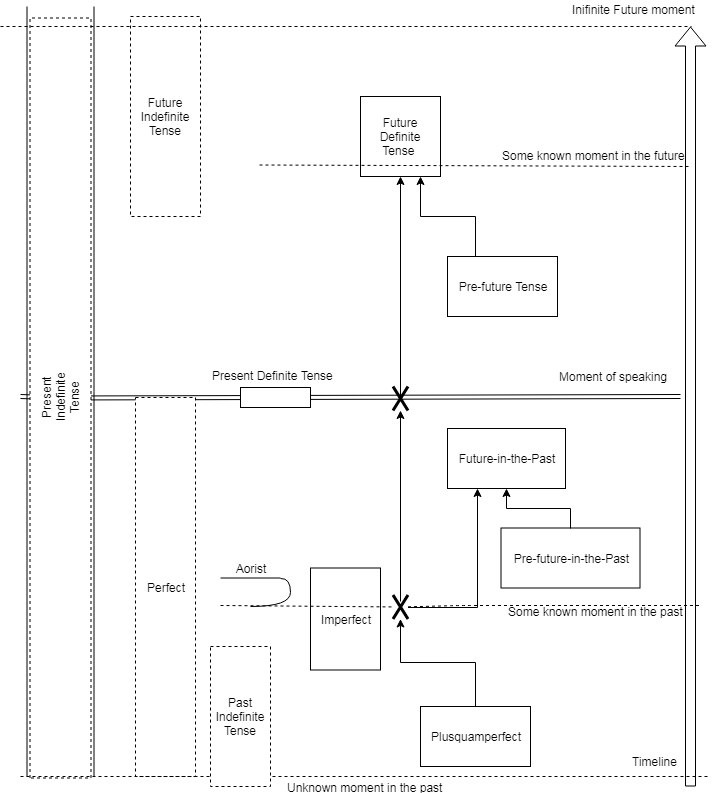
\includegraphics[width=\linewidth]{./sources/tenses.jpg}
	\caption{Tenses in Novoslovnica}
	\label{fig:tenses}
\end{figure}

Present group of tenses consists of Present Indefinite Tense (\textit{Pritomen čas}) and Present Definite Tense (\textit{Sëdyšen čas}).

Present Indefinite Tense\index{tense!present indefinite} (\textit{Pritomen čas}) is used when the action does not depend on time. For example, in the first example we know that the Earth always revolves and nothing but the apocalypsis can change it. This tense is very similar to the English one and has similar use cases. We can find this tense in indicative (examples 1, 2) and declarative (example 3, 4) moods mostly (in some cases it can be found in different moods too).

Note that in declarative there are two variants of present indefinite, because of its resultive semantics. In example 3 you can see the verb in declarative mood, in present indefinite tense, and in example 4 you can see the same tense and mood but within a predicateless sentence.

Also take care of the translation in example 3. You can mess it with English Present Perfect Tense (He has bought two cars), but this sentence should be translated with the verb «to have» in Present Indefinite with the participle III of the verb «to buy» (bought).

\textbf{Examples:}

\textit{Zemlä sę vreta okolo slånca.} - The Earth revolves around the Sun.

\textit{Vsękyǐ denj ja hođam do učilišta prez lěpyǐ park.} — Every day I walk to school through the beautiful park.

\textit{On imá kupeno dva vozidla.} — He has two cars bought.

\textit{Lěs i tïhota...} — There are forest and silence around me...

Present Definite Tense\index{tense!present definite} (\textit{Sëdyšen čas}) is used if the action depends on time. In the first example we can see a sentense with the following semantics: now I think about the rest, though in an hour I can forget about this thought.

Generally, this tense is close to Present Continuous Tense in English, though has a different interpretation. If you want to get in differences, we can give you such an example: «The Earth is revolving around the Sun at the moment». Read this hypothetic sentence that is syntaxicly valid in English.

What would be the differences of English and Novoslovnica here? It is in a term of differentiation. English operates with the time and Novoslovnica operates with the mutability. That is why here Novoslovnica will still use Present Indefinite Tense with the word «sëdy» (at the moment).

\textbf{Examples:}

\textit{Ja myslü o počïvkě.} — I am thinking about the rest.

\textit{On idaje do råboty, zato ne može da odgovori vam.} — He is going to the work, that is why he cannot answer you.

The group of future tenses comprises two ones: Future Tense and Pre-future Tense.

Future Definite Tense\index{tense!future definite} (\textit{Bųdešt čas}) defines that the action will appear in the future with reference with the moment of speaking. There are three variants of how you can use Future Tense in Novoslovnica.

Firstly, you can use the verb «hteti» (to will) in 3-person form with the main verb in Present Indefinite Tense (example 1). This varitant is most similar to English Future Simple Tense.

Secondly, you can use the verb «byti» (to be) with inifinitive form of the main verb (example 2). This variant is close to English Future Continuous Tense. It is often used with verbs of A-type (read the chapter about verbal types in Novoslovnica).

Finally, you can use a synthetic verb form with the future tense conjugation (example 3). In English, it should be translated in Future Simple so as the first one.

\textbf{Examples:}

\textit{Ja hte kazam ti něčto.} — I will tell you something.

\textit{Ja bųdu sluhati gudbu.} — I will listen to music. (I will be listening to music).

\textit{Nakonec ja tę viđahtem}. – Finally, I will meet you.

Pre-future Tense\index{tense!pre-future} (\textit{Predbųdešt čas}) is a grammatical tense that is used when the speaker should explicitly show that the action will take place before another future action. So, this tense deals with the comparison of future actions rather than with the moment of speaking.

In Novoslovnica Pre-future Tense is formed by using the verb «hteti» in 3-person form with the main verb in perfect form (examples 1, 2). This tense should be translated in English with Future Perfect Tense.

\textbf{Examples:}

\textit{Ja hte sòm kupil květy, dy ty hte priǐdaš do města.} — I will have bought flowers, when you come to the place.

\textit{On hte je zakončil učilišto, dy otec mu hte sę vreta dodomu}. — He will have graduated from school, when his father comes back home.

Future Indefinite Tense\index{tense!future indefinite} (\textit{Něĝdašen čas}) is a rather rare tense to be used in Novoslovnica. It has no direct equivalents in English and should be translated in Future Simple with some keywords (such as «somewhen», «ever», «once»). The sense of this tense is to show that the action takes place in a future moment or period of time, but we do not care of when it will occur or how long it will last.
This tense is formed by Pre-future form of the verb «byti» with the past passive participle of the main verb. Look at the examples to get acquainted.

\textbf{Examples:}

\textit{On hte je byl nagrådil medalom mę.} — Once he will grant me with a medal.

\textit{Ja hte sòm byl kupil vašu věčj.} — Once I will but your item.

All other tenses are related to the past period of time. Firstly, we will consider real past tenses and then future-in-the-past ones.

Aorist\index{tense!aorist} (\textit{Prost minul čas}) determines the fact of the committed action without semantic details. It is similar in usage with English Past Simple Tense. Using Aorist we consider only the time the action occurs, but do not think about its duration.

In Novoslovnica it is formed by verb-base vowels with past definite endings: «-h», «-ša», «-še», «-hma», «-hta», «-ha», «-hme», «-hte», «-hu».

\textbf{Examples:}

\textit{Ja dělah råbotu-ta včera.} — I did the work yesterday.

\textit{Pred dvě ročiny ja jěŝih v gråd-òt.} — Two years ago I travelled to the city.

Imperfect\index{tense!imperfect} (\textit{Neporęden minul čas}) determines the imperfect aspect of the past action. That means it is used with habitual, durable repeated actions etc, that took place in the past. Using imperfect we add the information, that our action took some exact time in the past. This tense is similar in usage with English Past Continuous Tense or Past Perfect.

It is formed so as Aorist with the one difference. There is a «-ě-» vowel before endings, not the verb-base vowel. So, for any verb type (see a chapter about verbal types) there is only a single imperfect form.

\textbf{Examples:}

\textit{Ja pišěh nadomnu råbotu dvě godiny včera.} — I was writing my homework for two hours yesterday.

\textit{Prijatelj mi ráděše na zavodu dvě ročiny.} — My friend had worked on a plant for two years.

Perfect\index{tense!prefect} (\textit{Svòršen minul čas}) determines the action has been committed before the present moment. That means, that we take account on the result of the action, on the fact it is finished, while Aorist determines the fact of the action itself and the time when it occured. So, it is a full equivalent of English Present Perfect Tense.

In Novoslovnica Perfect is formed by the auxiliary verb «byti» in Present Indefinite and an L-participle following it.

\textbf{Examples:}

\textit{On je izmyslïl novu ŧeoriju o problemě-ta.} — He has devised a new theory on the problem.

\textit{Môǐ brat je zakončil vysšojučilišto.} — My brother has graduated from University.

Plusquamperfect\index{tense!plusquamperfect} (\textit{Predminul čas}) determines the fact our action is further from us than another action in the past. It is akin Pre-Future tense, just with past actions. Simply speaking, it is an equivalent of English Past Perfect Tense. So as Pre-Future tense, actions in Plusquamperfect are usually used in pair with another past action that stands in Aorist.

Plusquamperfect in Novoslovnica is formed with aorist form of the auxiliary verb «byti» with an L-participle of the main verb.

\textbf{Examples:}

\textit{Ja byh doǐdal do ulicy-ta, dy on mi odŝvoniše, če ne može da priǐde.} — I had arrived to the street by the time he called be to say he cannot come.

\textit{On byše zdělal model, ĝda ja kazaše mu, če to ne máše potrěbnostï.} — He had done a model, when I told him it was unnecessary. 

Now we should consider two last tenses: Future-in-the-Past tense and Pre-Future-in-the-Past tense.

Future-in-the-Past tense (Bųdešt v minulom čas) is used when we speak about past actions, that occured after some other past actions. To emphasize this fact we use a past variant of the future tense — Future-in-the-Past. English has an equivalent, so it is easy to build a parallel between these two tenses. In Novoslovnica this tense is build with imperfect of the auxiliary verb «hteti» and DA-construction of the main verb (example 1).

This tense has also another meaning, that can be expressed with «would like to» phrase in English. It shows a polite intention to do something (example 2).

\textbf{Examples:}

\textit{My zapytahme dali vozidlo htěše da priǐde včas.} — We wondered if the bus would arrive on time.

\textit{Ja htěh da kazam ti něčto.} — I would like to say you something.

Pre-Future-in-the-Past Tense\index{tense!pre-future-in-the-past} (\textit{Predbųdešt v minulom čas}) is used, when we speak about some actions, that happened earlier than some future actions in the past (analogue of pre-future tense in the past). It has a similar meaning with Future-in-the-Past Perfect tense in English and it is rather rarely used.

It is formed with imperfect of the auxiliary verb «hteti» with perfect form of the main verb via DA-construction (look at the example).

\textbf{Examples:}

\textit{Vy kazahte, če htěhte da jeste podpisali pismo pred tym, kak htěhte da započïnate råbotati.} — You said you would have signed the paper before you would start working.

Past Indefinite Tense\index{tense!past indefinite} (\textit{Davnominul čas}) is the last official tense in Novoslovnica. It describes an action that occured in some moment in the past we do not know. In English we should translate it with Past Simple or with the «used to»-construction. It can be considered as a pair to Future Indefinite Tense.

\textbf{Examples:}

\textit{On je byl pisal knigu.} — He used to write a book.

Let us summarize all the equivalents of Novoslovnica's Tenses in English in the next table.

\begin{table}
	\caption{English equivalents of tenses in Novoslovnica}
	\begin{tabular}{ p{11em} p{11em} }
		\textbf{Tense in Novoslovnica}       & \textbf{English equivalent}                  \\
		Present Indefinite Tense             & Present Simple                               \\
		Present Definite Tense               & Present Continuous                           \\
		Future Indefinite Tense              & “once” + Future Simple                       \\
		Future Definite Tense (with “hteti”) & Future Simple                                \\
		Future Definite Tense (with “byti”)  & Future Continuous                            \\
		Future Definite Tense (single form)  & Future Simple                                \\
		Pre-future Tense                     & Future Perfect (Cont.)                       \\
		Future-in-the-Past Tense             & Future-in-the-Past Simple or “would like to” \\
		Pre-future-in-the-Past Tense         & Future-in-the-Past Perfect (Cont.)           \\
		Aorist                               & Past Simple                                  \\
		Perfect                              & Present Perfect (Cont.)                      \\
		Imperfect                            & Past Continuous                              \\
		Plusquamperfect                      & Past Perfect (Cont.)                         \\
		Past Indefinite Tense                & “used to”                                    
	\end{tabular}
\end{table}

The third verbal category can be found in Novoslovnica which is shown only in differences between Aorist and Imperfect: perfection, while other tenses differ only by determinacy and time. So, you can use complex tenses as Perfect, Plusquamperfect, Past Indefinite etc. with aorist and imperfect participles and receive two shades of perfection meaning.

\section{Mood}

% TODO: Check the correspondence with the article

Mood is a grammatical feature of verbs, used for signaling modality []. Mood is distinct from grammatical tense or grammatical aspect, although the same word patterns are used for expressing more than one of these meanings at the same time. There are several moods in Novoslovnica \cite{nsl-naklony}:

\begin{itemize}
	\item Indicative
	\item Declarative
	\item Subjunctive
	\item Conjunctive I
	\item Conjunctive II
	\item Imperative
	\item Optative
	\item Jussive
	\item Hortative
	\item Supine
	\item Inferential
\end{itemize}

Moods are divided into realis and irrealis moods. Realis mood is a grammatical mood which is used principally to indicate that something is a statement of fact. More precisely, it is used to express what the speaker considers to be a known state of affairs. Novoslovnica has two realis moods - indicative and declarative.

Indicative mood (\textit{Oznamitelnyǐ})  is used when we need simply to indicate that something is a statement of fact. Indicative has a variety of forms, including positive, negative and interrogative. Due to this fact it is chosen to be a basic mood, that is compared to the others. Indicative mood will be extensively considered in the next chapters. Just look at few examples.

\textbf{Examples:}

\textit{On glěděše iz prozorca doma si.} - He was looking out of the window of his house.

\textit{Ja bųdu hoditi vò vysšojučilišto črez dvě godiny.} - I will attend the university in two years.

Declarative mood (\textit{Objavitelnyǐ}) is used when we describe a state of something, considering the action it was caused by. Declarative mood is of the same degree of variety as indicative mood, though is not used as often as indicative.

The first difference with indicative mood is in using auxiliary verb “imáti” (to have) instead of “byti” (to be) while forming sentences. This makes some semantic shifts in Novoslovnica. Look at the second example: the auxiliary verb is used in present tense, though it has a resultive semantic value. For present semantics the verbless sentences are used (first example).

The second difference is in the particle being used with the auxiliary verb in two moods. In indicative we use L-particles, while in declarative mood we use passive ones.

\textbf{Examples:}

\textit{Rěka krasna i slånco.} - (There are) Beautiful river and the sun (around me).

\textit{Ja mám rođeno dvôh synoŭ.} - I have two sons born.

Subjunctive mood (\textit{Predpokladnyǐ}) is used when we want to express various states of unreality: wish, emotion, possibility, obligation etc. Subjunctives occur most often, although not exclusively, in subordinate clauses, using particles “aby”, “žeby”, “čtoby”, “išby” (example 1).

Take a note about absence of auxiliary verb while using L-particles. We just use a subjunctive particle with them. Though, we can also use infinitive instead of L-particle with the object in dative (example 2). Moreover, DA-forms can be used to express subjunctive (example 3). Nevertheless, there are cases you can use subjunctive in the main clause (example 4). 

\textbf{Examples:}

\textit{Az upëram aby ty odidal.} - I would like you to leave.

\textit{Az upëram aby ti odidati.} - It’s better for you to leave.

\textit{Ja htem da ty odidaš.} - I want you to leave.

\textit{Ty by odidal odde.} - You better leave here.

Conjunctive mood I (\textit{Domyselnyǐ}) is used to express real wishes relatively present moment. It means, using conjunctive I we show that our wish is still able to be implemented. It is a classic variant of conjunctive and is formed by conjunctive form of the verb “byti” (to be) with an L-participle.

In fact, this mood is rather similar to Conditional II in English with the same tense analogues used (examples 2, 3). If we use just conjunctive clause, it is similar with “wish-construction” usage area in English (example 1). However, we can express conjunctive with the single clause using past transgressive (example 4).

Note, that having two clauses we need to use conditional conjunctions (“ako”, “jestjli”, “koli”, “dali”, “či” etc.).

\textbf{Examples:}

\textit{Az bih htěl da viđu slånco v ovyǐ obvlåčnyǐ denj.} - I wish I see the sun in this cloudy day.

\textit{On biše doǐdal do nas, ako my zazovahme ĝo.} - He would come if we called him.

\textit{Ako znaše on novoslovnicu, mogal biše da govori so vsïmi slověnami.} - If he knew Novoslovnica, he would speak with all Slavs.

\textit{Znavšy novoslovnicu, on mogal biše da govori so vsïmi slověnami}. - If he knew Novoslovnica, he would speak with all Slavs.

Conjunctive mood II (\textit{Domyselnyǐ}) is the second conjunctive mood and it is used to express unreal wishes that have not been realized relatively a moment in the past. It can be formed by the verb “byti” in conjunctive form either  with supine (example 1) or with plusquamperfekt form of the main verb (example 2). It can be related to Conditional III in English. 

Note, that using supine you do not have to use conditional conjunctions between clauses. Moreover, we can use past active participle in the conditional clause (example 3). Attention! Compare this with the past transgressive in the single clause in Conjunctive I.

\textbf{Examples:}

\textit{Htětj da sę vidim s nim včera, bih byl mogal to da sdělam.} - If  I had wanted to see him yesterday, I would have meet him.

\textit{Ako byh htel da sę vidim s nim včera, bih byl mogal to da sdělam.} - If  I had wanted to see him yesterday, I would have meet him.

\textit{Ako byh htel da sę vidim s nim včera, bih byl mogavšym to sdělati.} - the same translation

Imperative mood (\textit{Zapovědnyǐ})  is used when we want to tell somebody a command or a request. In Novoslovnica it has only I-person (in dual and plural) and II-person (in singular, dual and plural) forms. It is indicated by special endings (look forward for details). In the examples you can see how imperative is used.

Please note that imperative is indicated only by single form. Complex forms are not of this mood.

\textbf{Examples:}

\textit{Piši ovu knigu.} - [Please] write this book. (you, sg)

\textit{Kažite mu poslanije-to.} - [Please] tell him the message. (you, pl)

\textit{Pročitaǐte ovu knigu.} - [Please] read this book. (you, pl)

\textit{Predgotuǐmo juž sëdy pokôǐ-ot.} - [Please] prepare the room now! (we, pl)

Optative mood (\textit{Žadatelnyǐ}) is a grammatical mood that expresses wish or hope. It is used when we want something or somebody to let us succeed in any action we are going to do. It is formed by DA-construction in the main clause (look at the examples). 

In English we can find similarity in LET-forms (examples 1, 2) or some general expressions that reveal our wish (example 3).

\textbf{Examples:}

\textit{Da daǐ mi pomognuti ti.} - Let me help you.

\textit{Da bųde tako.} - Let it be so.

\textit{Da žive Bòlĝarija.} - Long live Bulgaria.

Jussive mood (\textit{Umožnitelnyǐ}) is a grammatical mood of verbs for issuing orders and commanding. In Novoslovnica it is used to make orders for third-person expressions. There are no direct equivalents in English for this mood, but we can translate it with impersonal sentences (example 1) or with MUST-modal expressions. It is formed by indicative with “haǐ” modal word.

\textbf{Examples:}

\textit{Haǐ toǐ ne tòpta trevy.} - Do not walk on grass.

\textit{Haǐ on podide.} - He must come closer.

Hortative mood (\textit{Predložnyǐ})  is a grammatical mood that let verb express encourage or discourage of doing something. It can be translated with “let us” (encourage) or “might not” (discourage) constructions in English. In Novoslovnica it is formed with “něhaǐ” modal word with indicative and is able to have negative (example 4) and positive (examples 1-3) form. It is generally used just with I-person expressions.

\textbf{Examples:}

\textit{Něhaǐ grame v ovu gru.} - Let us play this game.

\textit{Něhaǐ pějama pěsnü.} - Let us (both) sing a song.

\textit{Něhaǐ govorim to otcu.} - I might say this to father.

\textit{Něhaǐ ne idame v dom-òt.} - We might not go into the house.


Supine (\textit{Dostęgatelnyǐ}) is rather a grammar form than a mood. Nevertheless, it is often used to express aiming something and the action of approaching to the goal that has been defined. It is similar to infinitive but the ending (infinitive has “-ti” ending, while supine has “-tj” endind). It is usually used with modal verbs and verbs of moving.

Supine can be translated in English through complex predicate. That is because in Novoslovnica supine is practically never used as a single verb form. It is generally used with main verb that determine the background action of the circumstance. Look at the examples to get acquainted with it.

\textbf{Examples:}

\textit{Moǐca je priǐdala povědatj dobru novinu.} - Mojca has come to message a good news.

\textit{Běgi skoro sę preoblekatj.} - Run fast to change clothes.

\textit{Poǐdame kupovatj.} - Let’s go to buy something.

Inferential mood (\textit{Prekazatelnyǐ}) is used to report an unwitnessed event without confirming it. It is often used in stories or fiction books and is very similar with indicative. The only difference is in 3-person in past tenses, where the auxiliary verb “byti” disappears and we use just L-participle. In English it should be translated with ordinary indicative (examples 1-4), sometimes “there”-forms also can be used (example 5). Not, that we use L-participle in Novoslovnica in the past tense (you can mess it with Perfect tense), while it should be translated in Past Simple.
Look at the examples.

\textbf{Examples:}

\textit{Jesòm mu ĝo kupil.} - I have bought it for him.

\textit{Byl sòm kupil naǐ-prosty martenicy, ale toǐ izbral naǐ-råzkošny.} - I had bought simpliest martenitsy, but he bought the most luxurious.

\textit{On byl bogatym.} - He was rich.

\textit{Kųde byl master?} - Where was the master?

\textit{Žila žena i mųž v malomu domu.} - There lived a woman and a man in a small house.

\section{Noun}

\begin{table}[h]
	\caption{Noun characteristics}
	\begin{tabular}{lllll}
		\textbf{Title}              & \textbf{Value}                            \\
		Semantic value              & Concept                                   \\
		Category                    & Independent                               \\
		Subcategory                 & Nominal                                   \\
		Alteration                  & Declension                                \\
		Alteration parameters       & Case, Numbers, Gender, Type of Declension \\
		Differentiation parameters  & Gender, Animacy, Types of  Declension                                  
	\end{tabular}
\end{table}

Nouns can be differentiated by three parameters: gender, animacy and the type of declension.

\underline{Animacy} determines whether the object is animate (we are able to ask “Who is it?” to the object) and inanimate (we are able to ask “What is it?” to the object).

\underline{Gender} determines whether the object is masculine, feminine or undefined (we cannot say it is one of the previous genders). Hence, there are three genders: masculine (with masculine properties), feminine (with feminine properties) and neutral (with undefined properties).

Despite English, Novoslovnica make us always show word gender explicitly of both animacies. We can say “it” to the object if we aren’t coupled with it in English. In Novoslovnica (as in every Slavic language) we should use the predefined gender when we speak about some concept (noun). Using wrong genders shows your ignorance and language nescience.

\underline{Type of declension} is a parameter of declension function. Declension is a function of word alteration. It has two input parameters - the word itself and the type of declension that includes the terms of animacy, gender and some morphological features (such as word endings) in it. The output is a list of forms that the noun can be changed into. Novoslovnica supports 27-cell output list with (3 numbers) * (9 cases) elements in it. Further you can see tables of different declension types. These tables cover all use cases of declension function.

P.S. In tables abbrevs “A” and “I” are for “animate” and “inanimate” respectively.


\begin{table}
	\caption{Hard feminine}
	\begin{tabular}{lllllll}
		\textbf{Ia Type}       
			& \multicolumn{2}{c}{Singular} 
				& \multicolumn{2}{c}{Dual} 
					& \multicolumn{2}{c}{Plural} \\
		& An.   & Inan.  & An.   & Inan.   & An.  & Inan. \\
		Nominative    & \multicolumn{2}{c}{-a}      
						& \multicolumn{2}{c}{-ě}        
							& \multicolumn{2}{c}{-y} \\
		Genitive      & \multicolumn{2}{c}{-y}       
						& \multicolumn{2}{c}{-oŭ}      
							& \multicolumn{2}{c}{-}   \\
		Partitive     & \multicolumn{2}{c}{-y}       
						& \multicolumn{2}{c}{-oŭ}      
							& \multicolumn{2}{c}{-} \\
		Accusative    & \multicolumn{2}{c}{-u}       
						& -ova & -ě
							& \multicolumn{2}{c}{-} \\
		Dative        & \multicolumn{2}{c}{-ě}       
						& \multicolumn{2}{c}{-oma}     
							& \multicolumn{2}{c}{-am} \\
		Instrumental  & \multicolumn{2}{c}{-oǐ}     
						 & \multicolumn{2}{c}{-ama}     
						 	& \multicolumn{2}{c}{-ami} \\
		Prepositional & \multicolumn{2}{c}{-ě}       
						& \multicolumn{2}{c}{-ověh}     
							& \multicolumn{2}{c}{-ěh} \\
		Locative      & \multicolumn{2}{c}{-jï}      
						& \multicolumn{2}{c}{-oŭ}       
							& \multicolumn{2}{c}{-ah} \\ 
		Vocative      & \multicolumn{2}{c}{-o}       
						& \multicolumn{2}{c}{-ove}      
							& \multicolumn{2}{c}{-ije}
	\end{tabular}
\end{table}


\begin{table}
	\caption{Hard masculine}
	\begin{tabular}{lllllll}
		\textbf{Ib Type}       
		& \multicolumn{2}{c}{Singular} 
		& \multicolumn{2}{c}{Dual} 
		& \multicolumn{2}{c}{Plural} \\
		& An.   & Inan.  & An.   & Inan.   & An.  & Inan. \\
		Nominative    & \multicolumn{2}{c}{-a}      
		& \multicolumn{2}{c}{-ě}        
		& \multicolumn{2}{c}{-y} \\
		Genitive      & \multicolumn{2}{c}{-y}       
		& \multicolumn{2}{c}{-oŭ}      
		& \multicolumn{2}{c}{-}   \\
		Partitive     & \multicolumn{2}{c}{-y}       
		& \multicolumn{2}{c}{-oŭ}      
		& \multicolumn{2}{c}{-} \\
		Accusative    & \multicolumn{2}{c}{-u}       
		& \multicolumn{2}{c}{-ě}
		& \multicolumn{2}{c}{-y} \\
		Dative        & \multicolumn{2}{c}{-ě}       
		& \multicolumn{2}{c}{-oma}     
		& \multicolumn{2}{c}{-am} \\
		Instrumental  & \multicolumn{2}{c}{-oǐ}     
		& \multicolumn{2}{c}{-ama}     
		& \multicolumn{2}{c}{-ami} \\
		Prepositional & \multicolumn{2}{c}{-ě}       
		& \multicolumn{2}{c}{-ověh}     
		& \multicolumn{2}{c}{-ěh} \\
		Locative      & \multicolumn{2}{c}{-jï}      
		& \multicolumn{2}{c}{-oŭ}       
		& \multicolumn{2}{c}{-ah} \\ 
		Vocative      & \multicolumn{2}{c}{-o}       
		& \multicolumn{2}{c}{-ove}      
		& \multicolumn{2}{c}{-ije}
	\end{tabular}
\end{table}

\begin{table}
	\caption{Soft feminine}
	\begin{tabular}{lllllll}
		\textbf{Ic Type}       
		& \multicolumn{2}{c}{Singular} 
		& \multicolumn{2}{c}{Dual} 
		& \multicolumn{2}{c}{Plural} \\
		& An.   & Inan.  & An.   & Inan.   & An.  & Inan. \\
		Nominative    & \multicolumn{2}{c}{-ä}      
		& \multicolumn{2}{c}{-ě}        
		& \multicolumn{2}{c}{-ï} \\
		Genitive      & \multicolumn{2}{c}{-ï}       
		& \multicolumn{2}{c}{-öŭ}      
		& \multicolumn{2}{c}{-ëǐ}   \\
		Partitive     & \multicolumn{2}{c}{-ï}       
		& \multicolumn{2}{c}{-öŭ}      
		& \multicolumn{2}{c}{-ëǐ} \\
		Accusative    & \multicolumn{2}{c}{-ü}       
		& \multicolumn{2}{c}{-ě}
		& \multicolumn{2}{c}{-i} \\
		Dative        & \multicolumn{2}{c}{-ě}       
		& \multicolumn{2}{c}{-ëma}     
		& \multicolumn{2}{c}{-äm} \\
		Instrumental  & \multicolumn{2}{c}{-ëǐ}     
		& \multicolumn{2}{c}{-äma}     
		& \multicolumn{2}{c}{-ämi} \\
		Prepositional & \multicolumn{2}{c}{-ě}       
		& \multicolumn{2}{c}{-ëvěh}     
		& \multicolumn{2}{c}{-ěh} \\
		Locative      & \multicolumn{2}{c}{-jï}      
		& \multicolumn{2}{c}{-öŭ}       
		& \multicolumn{2}{c}{-äh} \\ 
		Vocative      & \multicolumn{2}{c}{-ö}       
		& \multicolumn{2}{c}{-ëve}      
		& \multicolumn{2}{c}{-e}
	\end{tabular}
\end{table}

\begin{table}
	\caption{Soft masculine}
	\begin{tabular}{lllllll}
		\textbf{Id Type}       
		& \multicolumn{2}{c}{Singular} 
		& \multicolumn{2}{c}{Dual} 
		& \multicolumn{2}{c}{Plural} \\
		& An.   & Inan.  & An.   & Inan.   & An.  & Inan. \\
		Nominative    & \multicolumn{2}{c}{-ä}      
		& \multicolumn{2}{c}{-ě}        
		& \multicolumn{2}{c}{-ï} \\
		Genitive      & \multicolumn{2}{c}{-ï}       
		& \multicolumn{2}{c}{-öŭ}      
		& \multicolumn{2}{c}{-ëj}   \\
		Partitive     & \multicolumn{2}{c}{-ï}       
		& \multicolumn{2}{c}{-öŭ}      
		& \multicolumn{2}{c}{-ëǐ} \\
		Accusative    & \multicolumn{2}{c}{-ü}       
		& \multicolumn{2}{c}{-ëva}
		& \multicolumn{2}{c}{-ëvi} \\
		Dative        & \multicolumn{2}{c}{-ě}       
		& \multicolumn{2}{c}{-ëma}     
		& \multicolumn{2}{c}{-äm} \\
		Instrumental  & \multicolumn{2}{c}{-ëǐ}     
		& \multicolumn{2}{c}{-äma}     
		& \multicolumn{2}{c}{-ämi} \\
		Prepositional & \multicolumn{2}{c}{-ě}       
		& \multicolumn{2}{c}{-ëvěh}     
		& \multicolumn{2}{c}{-ěh} \\
		Locative      & \multicolumn{2}{c}{-jï}      
		& \multicolumn{2}{c}{-öŭ}       
		& \multicolumn{2}{c}{-äh} \\ 
		Vocative      & \multicolumn{2}{c}{-ö}       
		& \multicolumn{2}{c}{-ëvi}      
		& \multicolumn{2}{c}{-ïe}
	\end{tabular}
\end{table}

\begin{table}
	\caption{Hard masculine}
	\begin{tabular}{lllllll}
		\textbf{IIa Type}       
		& \multicolumn{2}{c}{Singular} 
		& \multicolumn{2}{c}{Dual} 
		& \multicolumn{2}{c}{Plural} \\
		& An.   & Inan.  & An.   & Inan.   & An.  & Inan. \\
		Nominative    & \multicolumn{2}{c}{-}      
		& \multicolumn{2}{c}{-a}        
		& \multicolumn{2}{c}{-y} \\
		Genitive      & \multicolumn{2}{c}{-a}       
		& \multicolumn{2}{c}{-oŭ}      
		& \multicolumn{2}{c}{-ov}   \\
		Partitive     & \multicolumn{2}{c}{-u}       
		& \multicolumn{2}{c}{-oŭ}      
		& \multicolumn{2}{c}{-ov} \\
		Accusative    & -a & -      
		& -ova & -a 
		& -ov & -y \\
		Dative        & \multicolumn{2}{c}{-u}       
		& \multicolumn{2}{c}{-ovi}     
		& \multicolumn{2}{c}{-am} \\
		Instrumental  & \multicolumn{2}{c}{-om}     
		& \multicolumn{2}{c}{-ama}     
		& \multicolumn{2}{c}{-ami} \\
		Prepositional & \multicolumn{2}{c}{-ě}       
		& \multicolumn{2}{c}{-ověh}     
		& \multicolumn{2}{c}{-ěh} \\
		Locative      & \multicolumn{2}{c}{-u}      
		& \multicolumn{2}{c}{-oŭ}       
		& \multicolumn{2}{c}{-ah} \\ 
		Vocative      & \multicolumn{2}{c}{-e}       
		& \multicolumn{2}{c}{-ove}      
		& \multicolumn{2}{c}{-ïe}
	\end{tabular}
\end{table}



\begin{table}
	\caption{Soft masculine}
	\begin{tabular}{lllllll}
		\textbf{IIb Type}       
		& \multicolumn{2}{c}{Singular} 
		& \multicolumn{2}{c}{Dual} 
		& \multicolumn{2}{c}{Plural} \\
		& An.   & Inan.  & An.   & Inan.   & An.  & Inan. \\
		Nominative    & \multicolumn{2}{c}{-j}      
		& \multicolumn{2}{c}{-ä}        
		& \multicolumn{2}{c}{-ï} \\
		Genitive      & \multicolumn{2}{c}{-ä}       
		& \multicolumn{2}{c}{-öŭ}      
		& \multicolumn{2}{c}{-ëǐ}   \\
		Partitive     & \multicolumn{2}{c}{-ü}       
		& \multicolumn{2}{c}{-öŭ}      
		& \multicolumn{2}{c}{-ëǐ} \\
		Accusative    & \multicolumn{2}{c}{-ä}     
		& \multicolumn{2}{c}{-ëva} 
		& \multicolumn{2}{c}{-ëǐ} \\
		Dative		  & \multicolumn{2}{c}{-ü}       
		& \multicolumn{2}{c}{-ëvi}     
		& \multicolumn{2}{c}{-äm} \\
		Instrumental  & \multicolumn{2}{c}{-ëm}     
		& \multicolumn{2}{c}{-äma}     
		& \multicolumn{2}{c}{-ämi} \\
		Prepositional & \multicolumn{2}{c}{-ě}       
		& \multicolumn{2}{c}{-ëvěh}     
		& \multicolumn{2}{c}{-ěh} \\
		Locative      & \multicolumn{2}{c}{-ü}      
		& \multicolumn{2}{c}{-öŭ}       
		& \multicolumn{2}{c}{-äh} \\ 
		Vocative      & \multicolumn{2}{c}{-ü}       
		& \multicolumn{2}{c}{-ëve}      
		& \multicolumn{2}{c}{-ïe}
	\end{tabular}
\end{table}



\begin{table}
	\caption{Hard neutral}
	\begin{tabular}{lllllll}
		\textbf{IIc Type}       
		& \multicolumn{2}{c}{Singular} 
		& \multicolumn{2}{c}{Dual} 
		& \multicolumn{2}{c}{Plural} \\
		& An.   & Inan.  & An.   & Inan.   & An.  & Inan. \\
		Nominative    & \multicolumn{2}{c}{-o}      
		& \multicolumn{2}{c}{-a}        
		& \multicolumn{2}{c}{-y} \\
		Genitive      & \multicolumn{2}{c}{-a}       
		& \multicolumn{2}{c}{-oŭ}      
		& \multicolumn{2}{c}{-}   \\
		Partitive     & \multicolumn{2}{c}{-u}       
		& \multicolumn{2}{c}{-oŭ}      
		& \multicolumn{2}{c}{-} \\
		Accusative    & \multicolumn{2}{c}{-o}     
		& \multicolumn{2}{c}{-a} 
		& \multicolumn{2}{c}{-y} \\
		Dative        & \multicolumn{2}{c}{-u}       
		& \multicolumn{2}{c}{-ovi}     
		& \multicolumn{2}{c}{-am} \\
		Instrumental  & \multicolumn{2}{c}{-om}     
		& \multicolumn{2}{c}{-ama}     
		& \multicolumn{2}{c}{-ami} \\
		Prepositional & \multicolumn{2}{c}{-ě}       
		& \multicolumn{2}{c}{-ověh}     
		& \multicolumn{2}{c}{-ěh} \\
		Locative      & \multicolumn{2}{c}{-u}      
		& \multicolumn{2}{c}{-oŭ}       
		& \multicolumn{2}{c}{-ah} \\ 
		Vocative      & \multicolumn{2}{c}{-e}       
		& \multicolumn{2}{c}{-ove}      
		& \multicolumn{2}{c}{-ïe}
	\end{tabular}
\end{table}

\begin{table}
	\caption{Soft neutral}
	\begin{tabular}{lllllll}
		\textbf{IId Type}       
		& \multicolumn{2}{c}{Singular} 
		& \multicolumn{2}{c}{Dual} 
		& \multicolumn{2}{c}{Plural} \\
		& An.   & Inan.  & An.   & Inan.   & An.  & Inan. \\
		Nominative    & \multicolumn{2}{c}{-ë}      
		& \multicolumn{2}{c}{-ä}        
		& \multicolumn{2}{c}{-ï} \\
		Genitive      & \multicolumn{2}{c}{-ä}       
		& \multicolumn{2}{c}{-öŭ}      
		& \multicolumn{2}{c}{-ëǐ}   \\
		Partitive     & \multicolumn{2}{c}{-ü}       
		& \multicolumn{2}{c}{-öŭ}      
		& \multicolumn{2}{c}{-ëǐ} \\
		Accusative    & \multicolumn{2}{c}{-ë}     
		& \multicolumn{2}{c}{-ä} 
		& \multicolumn{2}{c}{-ï} \\
		Dative		  & \multicolumn{2}{c}{-ü}       
		& \multicolumn{2}{c}{-ëvi}     
		& \multicolumn{2}{c}{-äm} \\
		Instrumental  & \multicolumn{2}{c}{-ëm}     
		& \multicolumn{2}{c}{-äma}     
		& \multicolumn{2}{c}{-ämi} \\
		Prepositional & \multicolumn{2}{c}{-ě}       
		& \multicolumn{2}{c}{-ëvěh}     
		& \multicolumn{2}{c}{-ěh} \\
		Locative      & \multicolumn{2}{c}{-ü}      
		& \multicolumn{2}{c}{-öŭ}       
		& \multicolumn{2}{c}{-äh} \\ 
		Vocative      & \multicolumn{2}{c}{-ü}       
		& \multicolumn{2}{c}{-ëve}      
		& \multicolumn{2}{c}{-ïe}
	\end{tabular}
\end{table}

\begin{table}
	\caption{Soft feminine}
	\begin{tabular}{lllllll}
		\textbf{IIIa Type}       
		& \multicolumn{2}{c}{Singular} 
		& \multicolumn{2}{c}{Dual} 
		& \multicolumn{2}{c}{Plural} \\
		& An.   & Inan.  & An.   & Inan.   & An.  & Inan. \\
		Nominative    & \multicolumn{2}{c}{-j}      
		& -erě & -ě        
		& -eri & -i \\
		Genitive      & -eri & -i 
		& -eröŭ & -öŭ
		& -erëǐ & -ëǐ \\
		Partitive     & -eri & -i 
		& -eröŭ & -öŭ
		& -erëǐ & -ëǐ \\
		Accusative    & -erj & -j     
		& -erëva & -ě
		& -erëǐ & -ï  \\
		Dative		  & -eri & -i
		& -erëma & -ëma 
		& -eräm & -äm \\  
		Instrumental  & -erïü & -ïü     
		& -eräma & -äma   
		& -erämi & -ämi \\
		Prepositional & -erě & -ě   
		& -erëvěh & -ëvěh     
		& -erěh & -ěh \\
		Locative      & -erjï & -j      
		& -eröŭ & -öŭ
		& -eräh & -äh \\
		Vocative      & \multicolumn{2}{c}{-ï}       
		& -erëve & -ëve
		& -erïe & -ïe 
	\end{tabular}
\end{table}

\begin{table}
	\caption{Soft neutral}
	\begin{tabular}{lllllll}
		\textbf{IIIb Type}       
		& \multicolumn{2}{c}{Singular} 
		& \multicolumn{2}{c}{Dual} 
		& \multicolumn{2}{c}{Plural} \\
		& An.   & Inan.  & An.   & Inan.   & An.  & Inan. \\
		Nominative    & \multicolumn{2}{c}{-ę}      
		& -ęta  & -eni        
		& -ęty & -eny \\
		Genitive      & -ęti & -eni 
		& -ętoŭ & -enoŭ
		& -ęt & -en \\
		Partitive     & -ęti & -eni 
		& -ętoŭ & -enoŭ
		& -ęt & -en \\
		Accusative    & -ęto & -ę     
		& -ętova & -ena
		& -ęt & -eny  \\
		Dative		  & -ęti & -eni
		& -ętovi & -enovi 
		& -ętam & -enam \\  
		Instrumental  & -ętëm & -enëm     
		& -ętama & -enama   
		& -ętami & -enami \\
		Prepositional & -ętě & -eně   
		& -ętověh & -enověh     
		& -ętěh & -eněh \\
		Locative      & -ętjï & -enjï      
		& -ętoŭ & -enoŭ
		& -ętah & -enah \\
		Vocative      & \multicolumn{2}{c}{-ų}       
		& -ętove & -enove
		& -ętïe & -ïe 
	\end{tabular}
\end{table}

\section{Adjective}

\begin{table}[h]
	\caption{Adjective characteristics}
	\begin{tabular}{lllll}
		\textbf{Title}              & \textbf{Value}               \\
		Semantic value              & Attribute                    \\
		Category                    & Independent                  \\
		Subcategory                 & Nominal                      \\
		Alteration                  & Declension                   \\
		Alteration parameters       & Case, Number, Gender, Degree \\
		Differentiation parameters  & Gender, Type, Form
	\end{tabular}
\end{table}

Adjective is one of POS that determines an attribute of the concept. There are two types of adjectives - relative and qualitative. 

Relative adjectives are called so, because they show relations between two concepts or a concept and an action.

\textbf{Examples:}

\textit{South (adj) pole} = South (noun) <= relation <= Pole

\textit{Južnyǐ pôl} = Jug <= relation <= Pôl

Qualitative adjectives are called so, because they show the quality of a concept’s property. This quality could be relative or quantitative or purely qualitative (showing concept condition, position, measure etc).

\textbf{Examples:}

\textit{Blue sky} = Sky => is (quality) => blue (attribute)

\textit{Sine nebo} = Nebo => is (quality) => sine (attribute) 

There is the only type of adjective declension. However, we will divide declension tables by gender and base softness.

\begin{table}[!htb]
	\caption{Masculine}
	\begin{tabular}{lllllll}
		\textbf{Masculine}       
		& \multicolumn{2}{c}{Singular} 
		& \multicolumn{2}{c}{Dual} 
		& \multicolumn{2}{c}{Plural} \\
		& Hard   & Soft  & Hard   & Soft   & Hard  & Soft \\
		Nominative    & -yǐ & -ïǐ     
		& -aja  & -äja        
		& -yji & -ïji \\
		Genitive      & -oga & -ëga 
		& -oŭ & -oŭ
		& -yh & -ïh \\
		Partitive     & -ogu & -ëgu 
		& -oŭ & -oŭ
		& -yh & -ïh \\
		Accusative    & -ogo & -ëgo     
		& -aja & -äja
		& -yji* & -ïji*  \\
		Dative		  & -omu & -ëmu
		& -oma & -ëma 
		& -ym & -ïm \\  
		Instrumental  & -ym & -ïm     
		& -yma & -ïma   
		& -ymi & -ïmi \\
		Prepositional & -om & -ëm  
		& -yvěh & -ïvěh     
		& -ěh & -ěh \\
		Locative      & -omu & -ëmu      
		& -oŭ & -oŭ
		& -yh & -ïh \\
		Vocative       & -yǐ & -ïǐ     
		& -aja  & -äja        
		& -yji & -ïji 
	\end{tabular}
\end{table}


\begin{table}[!htb]
	\caption{Feminine}
	\begin{tabular}{lllllll}
		\textbf{Feminine}       
		& \multicolumn{2}{c}{Singular} 
		& \multicolumn{2}{c}{Dual} 
		& \multicolumn{2}{c}{Plural} \\
		& Hard   & Soft  & Hard   & Soft   & Hard  & Soft \\
		Nominative    & -aja & -äja     
		& \multicolumn{2}{c}{-ěja}        
		& -yje & -ïje \\
		Genitive      & -oji & -ëji
		& -oŭ & -öŭ
		& -yh & -ïh \\
		Partitive    & -oji & -ëji
		& -oŭ & -öŭ
		& -yh & -ïh \\
		Accusative    & -uju & -üju     
		& \multicolumn{2}{c}{-ěja} 
		& -yje* & -ïje*  \\
		Dative		  & -oǐ & -ëǐ
		& -oma & -ëma 
		& -ym & -ïm \\  
		Instrumental  & -oju & -ëju
		& -yma & -ïma   
		& -ymi & -ïmi \\
		Prepositional  & -oǐ & -ëǐ
		& -yvěh & -ïvěh     
		& -ěh & -ěh \\
		Locative      & -oji & -ëji      
		& -oŭ & -oŭ
		& -yh & -ïh \\
		Vocative      & -aja & -äja     
		& \multicolumn{2}{c}{-ěja}        
		& -yje & -ïje 
	\end{tabular}
\end{table}

\begin{table}[!htb]
	\caption{Neutral}
	\begin{tabular}{lllllll}
		\textbf{Neutral}       
		& \multicolumn{2}{c}{Singular} 
		& \multicolumn{2}{c}{Dual} 
		& \multicolumn{2}{c}{Plural} \\
		& Hard   & Soft  & Hard   & Soft   & Hard  & Soft \\
		Nominative    & -oje & -ëje     
		& -aja  & -äja        
		& -yje & -ïje \\
		Genitive      & -oga & -ëga 
		& -oŭ & -oŭ
		& -yh & -ïh \\
		Partitive     & -ogu & -ëgu 
		& -oŭ & -oŭ
		& -yh & -ïh \\
		Accusative    & -ogo & -ëgo     
		& -aja & -äja
		& -yji* & -ïji*  \\
		Dative		  & -omu & -ëmu
		& -oma & -ëma 
		& -ym & -ïm \\  
		Instrumental  & -ym & -ïm     
		& -yma & -ïma   
		& -ymi & -ïmi \\
		Prepositional & -om & -ëm  
		& -yvěh & -ïvěh     
		& -ěh & -ěh \\
		Locative      & -omu & -ëmu      
		& -oŭ & -oŭ
		& -yh & -ïh \\
		Vocative       & -oje & -ëje     
		& -aja  & -äja        
		& -yje & -ïje 
	\end{tabular}
\end{table}

\subsection{Full and short adjectives}

There are two forms of adjectives: full and short.

We can find differences in using short and full forms of adjectives only in some cases - Nominative and Accusative. In other cases short adjectives correspond with appropriate full form adjective.

To understand how to change a full adjective to receive its short form look at the next table (C is for “consonant”, V is for “vowel”).

\begin{table}
	\begin{tabular}{ll}
		Full form adjective endings & Short form adjective endings \\
		C + C + yǐ & C + ò C \\
	    V + C + yǐ & V + C \\
		aja & a \\
		oje  & o \\
		yje & y \\
	\end{tabular}
\end{table}

Etymologically full adjectives date back to combined form of an adjective itself (short form) and a pronoun \footnote{Such a phenomenon existed in Russia, Belorussian and Baltic languages. A similar phenomenon is used in Macedonia today. Though a "pronoun-article" is used mostly with verb as in the following sentence.}. 

What about using full and short adjectives… There are some recommendations that you should follow in your speech. I tried to unite them into one table with cases when you should use either full form or short one.

\begin{table}
	\begin{tabular}{ll}
		Full form & Short form \\
		Before the modified noun & In a complex predicate \\
		In denominative sentence & - \\
	\end{tabular}
\end{table}


\subsection{Degrees of comparison}

When we speak about qualitative adjectives, we use a term of a degree of comparison. It’s the condition whether temporal adjective is greater in its measure than another one or not. There are three degrees: positive, comparative and superlative.

\underline{Positive} (or neutral, basic) degree is used when we do not mind about the comparison with other attributes. We could call it an undefined degree.

\underline{Comparative} degree is used when our attribute is greater than another one (attributes must be comparable).  

\underline{Superlative} degree is used when our concept has the attribute with most valuable degree in considered area.

There are two ways of comparison - synthetic and analytic. Synthetic comparison changes the word itself, while analytic comparison uses analytic constructions with other words to create a degree of comparison. You can you both analytic or synthetic comparison forms in your speech.

\textbf{Synthetic comparison}

Comparative degree can be formed in two ways: 

\begin{itemize}
	\item Adding between word base and word ending “-š-”, that means that the attribute has a more strongly pronounced property than another concept, expressed by a noun.
	\item Adding suffix “-š-” plus suffix “-ëǐ-” for soft word base and suffix “-aǐ-” for hard word base before it.
\end{itemize}

\textbf{Examples:}

Bolïǐ – boljšyǐ. Mnogyǐ - mnogšyǐ. Vëlïkyǐ - vëlïkšyǐ.

Bolïǐ – bolëǐšyǐ. Mnogyǐ - množaǐšyǐ. Vëlïkyǐ - vëlïčaǐšyǐ.

Superlative degree also has two variants, that are formed by adding a prefix “-naǐ-” to the comparative form. This prefix has a similar meaning with the English word “most”.

\textbf{Examples:}

Bolïǐ – boljšyǐ - naǐboljšyǐ. Mnogyǐ - mnogšyǐ - naǐmnogšyǐ. Vëlïkyǐ - vëlïkšyǐ - naǐvëlïkšyǐ.

Bolïǐ – bolëǐšyǐ - naǐbolëǐšyǐ. Mnogyǐ - množaǐšyǐ - naǐmnožaǐšyǐ. Vëlïkyǐ - vëlïčaǐšyǐ - naǐvëlïčaǐšyǐ.

Some says Novoslovnica has five degrees of comparison instead of three degrees with doubly forms. Let us know this classification.

\begin{itemize}
	\item \textit{Positive} degree equals to the one in ordinary classification. (Bolïǐ)

	\item \textit{Defined Comparative} degree matches the first variant of comparative form in ordinary classification. It is used when there are two objects and the temporal one has a prevailed property to another one. (\textit{Bolïšyǐ})

	\item \textit{Undefined Comparative} degree matches the second variant of comparative form in ordinary classification. It is used when we have some objects (more than two) and temporal object has a prevailed property to a few objects in the set (probably its power is an undefined number). (\textit{Bolëǐšyǐ})

	\item \textit{Relative superlative} degree matches the first variant of superlative form in ordinary classification. It is used when temporal object is in the set and has a superior property in it, but we cannot say that this property would have a superior value in other sets. (\textit{Naǐboljšyǐ})

	\item \textit{Absolute superlative} degree matches the second variant of superlative form in ordinary classification. It is used when there are no doubts in superiority of the temporal object’s property. (\textit{Naǐbolëǐšyǐ})
\end{itemize}

\textbf{Analytic forms}

There are two variants of how to use analytic comparison of adjectives: to use prefixes or to use an auxiliary adverb.

To create a comparative or a superlative form you should add a prefix “po-” or “naǐ-” respectively to the word though a defis.

\textbf{Examples:}

Kråtkyǐ - po-kråtkyǐ - naǐ-kråtkyǐ

Sïlnyǐ - po-sïlnyǐ - naǐ-sïlnyǐ

Analytic comparison forms have only three ones - positive, comparative and superlative. Analytic comparison with an auxiliary adverb is formed by adding to the positive form of the adjective a comparative or a superlative form of an auxiliary adverb (look at the paragraph about adverb degrees of comparison). However, you cannot use analytic comparison with adjectives “bolïǐ” and “mënïǐ”, because they are the basic forms of these auxiliary adverbs.

\textbf{Examples:}

Kråtkyǐ - bolěǐ kråtkyǐ - naǐbolěǐ kråtkyǐ

Bolïǐ - bolěǐ bolïǐ (\textbf{you cannot do that}!)

\section{Pronoun}

\begin{table}[!hbt]
	\caption{Pronoun characteristics}
	\begin{tabular}{lp{12em}}
		\textbf{Title}              & \textbf{Value}               \\
		Semantic value              & Attribute, Concept           \\
		Category                    & Independent                  \\
		Subcategory                 & Nominal                      \\
		Alteration                  & Declension                   \\
		Alteration parameters       & Case, Numbers, Gender, Person\\
		Differentiation parameters  & Gender, Type, Group
	\end{tabular}
\end{table}

Pronoun\index{pronoun} is a POS that has different meanings. It can play the role of an attribute or a concept, depending on what is replaced with the pronoun. However, pronoun has a verbal property of person.

Pronouns are divided into three types: nominal\index{pronoun!nominal} (noun-like declension), substantive\index{pronoun!substantive} (substantive declension), attributive\index{pronoun!attributive} (adjective-like declension).

There are also several groups of pronouns, depending on their semantic value. They are: personal, possessive, interrogative, relative, indefinite, definitive, reflexive, demonstrative, negative, reciprocal.

\subsection{Personal pronouns}

Personal pronouns\index{pronoun!personal} are one of the most important groups in the Pronoun POS. They replace nouns in sentences when we try to avoid an unreasonable repeat. Personal pronouns have different forms for every person-number cell. In the table you can see them.

\begin{table}[!htb]
	\begin{tabular}{llll}
		& Singular & Dual & Plural \\
		1 person & Ja (Az) & Ma & My \\
		2 person & Ty & Va & Vy \\
		3 person, ms & On & Ona & Oni \\
		3 person, fm & Ona & One & Oně \\
		3 person, neu & Ono & Oná & Onji
	\end{tabular}
\end{table}

I should mention the form “Vy” (You). As in English or polite Russian, we can use this pronoun for a single person when we want to emphasize our respect to the interlocutor. Moreover, we also have to use a plural form of the verb while speaking “Vy” in polite form.

Also you can see two forms of the 1 person - singular pronoun (I). Etymologically the form “Az” is full while “Ja” is only a short one. However, different Slavic languages have retained different forms and now we see Novoslovnica should support both ones. In Novoslovnica the difference between using “Az” and “Ja” lies in phonetics. As you see, “Az” begins with the vowel and ends with a consonant, “Ja” - controversially. If we remember rule 1 we will get such a list of rules:

\begin{itemize}
	\item If the word before the pronoun ends with a vowel and the word after begins with a consonant - you should use “Ja”
	\item If the word before the pronoun ends with a consonant and the word after begins with a vowel - you should use “Az”
	\item In other cases you can use either one or another variant\footnote{“Az” is more formal than “Ja”. In everyday speech you should use "Ja" variant while in scientific, official only "Az" should be used.}
\end{itemize}

Now let us speak about declension of personal pronouns. Personal pronouns relate to nominal pronouns (with noun-like declension). This is the most difficult type to learn.\footnote{The declension of personal pronouns is derived mostly from old-Slavonic language except for 1 person dual. The similar declension within still languages can be found in Slovenian.} But everything has its order and beauty.

Look for the tables in the eighth chapter.

\subsection{Reflexive pronoun}

This\index{pronoun!reflexive} is a separate group of pronouns. There is the only reflexive pronoun in Novoslovnica - “sebę”. Its feature is the absence of nominative form. It has only 7 cases to be alternated. Vocative and Nominative are absent.

\begin{table}[!htb]
	\begin{tabular}{lll}
		Case & Full & Short \\
		Genitive & Sebę & Sę \\
		Partitive & Sebä & Sä \\
		Accusative & Sebe & Se \\
		Dative & Sebi & Si \\ 
		Insrumental & Sobom (Soboǐ) & - \\ 
		Prepositional & O sobě & - \\
		Locative & V sobu & -
	\end{tabular}
\end{table}


“\textit{Sę}” is used very often as a reflexive suffix in verbs. It determines a way of creating medial voice sentences (look the paragraph about it).

However, there is a term of a complex reflexive form (CRF) also. It is formed by the sequence of a personal pronoun and the definitive pronoun “sám”. This form shows a partly-developed reflection of a subject.  

\textbf{Examples:}

\textit{On sám stroji búdu-ta.} -

\textit{On sę stroji.}

\textit{Búda-ta sę stroji nim.}

There is practically no difference in using a reflexive pronoun or a complex reflexive form. However, it is recommended to us a CRF for Nominative and to use a reflexive pronoun in other cases.

\subsection{Possessive pronouns}

Possessive\index{pronoun!possessive} pronouns show whom any object belongs to. For example, we can say “\textit{It is a thing of Bob} (which Bob possesses)”. In Novoslovnica you can use a similar expression: “\textit{To je věčj Boba}” (remember rules of case using). Also Novoslovnica has another expression with a possessive adjective: “To je Bobóva věčj”. This adjective shows that this thing belongs to Bob. However, if we have already used the name of Bob in our sentence, we should not repeat it again. English also uses possessive pronouns in such cases: “\textit{Bob is my friend and that’s his thing}”. We do not repeat the word Bob, we just say - his (which he possesses). That is what the possessive pronouns look like.

These pronouns are attributive, so we have no need to rewrite their declension, just to name nominative forms. Further, you take a nominative form of a possessive pronoun, look through declension tables for adjectives and transform your pronoun so as you did it with an adjective. Now let us look at the nominative forms of possessive pronouns.

\begin{table}[!htb]
	\caption{Possessive pronouns}
	\begin{tabular}{llll}
		& Singular & Dual & Plural \\
		1 person & Môǐ & Naš & Naš \\
		2 person & Tvôǐ & Vaš & Vaš \\
		3 person, ms & Jegôǐ & Onyš & Ih \\
		3 person, fm & Jejôǐ & Oneš & Ih \\
		3 person, neu & Jegôǐ & Onyš & Ih
	\end{tabular}
\end{table}

There also exists possessive adjectives you can see on the next table.

\begin{table}[!htb]
	\caption{Possessive adjective}
	\begin{tabular}{llll}
		& Singular & Dual & Plural \\
		1 person & Môǐnyǐ & Našnyǐ & Našnyǐ \\
		2 person & Tvôǐnyǐ & Vašnyǐ & Vašnyǐ \\
		3 person, ms & Jegôǐnyǐ & Onyšnyǐ & Ihnyǐ \\
		3 person, fm & Jejôǐnyǐ & Onešnyǐ & Ěhnyǐ \\
		3 person, neu & Jegôǐnyǐ & Onyšnyǐ & Ihnyǐ
	\end{tabular}
\end{table}

Possessive adjectives are used only in full form to underline the importance of something. Usually, possessive pronouns should be used.

Look at the examples to see the differences.

\textit{Môǐ pes lübi męso} - My dog likes meet.

\textit{Môǐnyǐ pes lübi męso} - My dog (that we are talking about now) likes meet.

Possessive forms (adjectives and pronouns) should be placed right before the identified word. Nevertheless, you can use a postfix form to describe possessiveness. In that case, you should use personal pronoun in Dative in role of a possessive one. Look at the examples.

\textit{Daǐte moju knigu - Daǐte knigu mi} (the latter is not recommended due to possible misunderstanding)

\textit{Ja  sòm poslal syna mi do pěkarnï - Ja sòm poslal mojoga syna do pěkarnï.}

As you see, such a form does not decline along with the main word. In the following table you can find the correlations between declinable prefix form and a "frozen" postfix one.

\begin{table}[!htb]
	\begin{tabular}{ll}
		\textbf{Prefix} & \textbf{Postfix} \\
		Môǐ & Mi \\
		Tvôǐ & Ti \\
		Svôǐ & Si \\
		Jegôǐ & Mu \\
		Jejôǐ & Ji \\
		Naš & Nam / Nama \\
		Vaš & Vam / Vama \\
		Jih & Jim \\
		Onyš & Onama \\
		Oneš & Oněma \\
	\end{tabular}
\end{table}

Note that the postfix form is pretty similar with use of genitive. The dative possessive form is used mostly in fiction texts to underline the beauty of writing. However, dative for singular pronouns is more frequently used than the genitive one.

\textbf{Examples:}

\textit{To je moja kniga} (Possessive pronoun) - Frequently used

\textit{To je kniga mi} (Dative) - Frequently used

\textit{To je kniga mę} (Genitive) - Rarely used

\textit{On je syn naju} (Genitive) - Frequently used

\textit{On je naš syn} (Possessive pronoun) - Frequently used

\textit{On je syn nama} (Dative) - Rarely used

\subsection{Interrogative and relative pronouns}

Interrogative\index{pronoun!interrogative} pronouns are used when we create a question. They are never in plural or dual. Also they have no declension. The only role of interrogative pronouns is to reveal an aim of the question (How much? Who? What?) - to guide the interlocutor to the right answer (you need).

Relative\index{pronoun!relative} pronouns aim is to introduce a relative clause.

\textit{Relative clause}\index{clause!relative} is a special kind of subordinate clause whose primary function is as modifier to a noun or nominal. We examine the case of relative clause modifiers in NPs first, and then extend the description to cover less prototypical relative constructions.\cite{english-grammar}

Interrogative and relative pronouns are practically the same, only usage differs, that is why I talk about them in the same paragraph. Let us look at them in the table.

\begin{table}[!htb]
	\begin{tabular}{p{8em}p{8em}p{8em}}
		English equivalent & Interrogative pronoun & Relative pronoun \\
		Who & Kto? & Ke \\
		What & Čto & Če \\
		What & Kakyǐ? & Kak \\
		Which & Ktoryǐ? & Ktor \\
		Whose & Čyǐ? & Čyǐ \\
		What & Jakyǐ? & Jak \\
		What & Kakvyǐ ? & Kakòv \\
		What & Kolïkyǐ ? & Kolïk 
	\end{tabular}
\end{table}

Pronouns “Kto”, “Čto” have a similar declension with possessive pronouns. Other pronouns decline so as adjectives do.
  
\subsection{Indefinite and negative pronouns}

Another group of pronouns that are similar to each other are indefinite\index{pronoun!indefinite} and negative\index{pronoun!negative} pronouns. They are derived from interrogative pronouns by adding the negative “ni-” and the indefinite “ne-” prefixes. Their declension equals to their ancestor’s one.

\begin{table}[!htb]
	\begin{tabular}{p{8em}p{8em}p{8em}}
		Interrogative pronoun & Negative pronoun & Indefinite pronoun \\
		Kto? & Nikto & Někto \\
		Čto & Ničto & Něčto \\
		Kakyǐ? & Nikakyǐ & Někakyǐ \\
		Ktoryǐ? & Niktoryǐ & Něktoryǐ \\
		Čyǐ? & Ničyǐ & Něčyǐ 
	\end{tabular}
\end{table}

\subsection{Demonstrative pronouns}

Demonstrative\index{pronoun!demonstrative} pronouns are usually used to make the interlocutor pay attention to something.
There are only four demonstrative pronouns. And this topic is closely connected with the articles. In the table 4.20 you can see these pronouns, divided by the terms of visibility and distance of the object with respect of the speaker.


\begin{table}[!htb]
	\caption{Demonstrative pronouns}
	\begin{tabular}{lll}
		& Visible & Invisible \\
		Far & Onyǐ & Tyǐ \\
		Close & Ovyǐ & Sïǐ  
	\end{tabular}
\end{table}

These pronouns decline so as adjectives do, so that is very easy. Nouns that are used with demonstrative pronouns should not be determinized with article. You should use \underline{either} demonstrative pronoun or articles.

\textbf{Examples:}

\textit{Onyǐ stol je starym} - That table (you are looking at) is old.

\textit{Stol-òn je star} - The table is old.

\textit{Ova kniga je korystnoǐ} - This book is interesting.

\textit{Kniga-va je korystna} - The book is interesting.

\subsection{Attributive pronouns}

Attributive\index{pronoun!definitive} pronouns indicate a generalized feature of an object. 

\begin{table}[!htb]
	\caption{Attributive pronouns}
	\begin{tabular}{ll}
		English equivalent & Definitive pronoun \\
		Whole & Vesj \\
		All & Vsë, vsä, vsï \\
		Every & Vsękyǐ, lübyǐ \\
		Each & Káždyǐ \\
		Another, other & Ïnyǐ, drugyǐ \\
		Both & Oba, obě \\
		Reflexive pronouns & Personal pronouns + sám
	\end{tabular}
\end{table}

All these pronouns decline as adjectives. I should say just about the last one - the pronoun “sám”. This pronoun is used with personal pronouns to create a complex reflexive form (look paragraph about reflexive pronouns). However, it keeps adjective-like declension.

\subsection{Reciprocal pronouns}


The last type of pronouns is reciprocal\index{pronoun!reciprocal}. It is used to refer to a noun phrase mentioned earlier in a sentence. English has only two such pronouns - each other and another one.

Slavic languages have much more variants:

\textit{Drug so drugom} - With each other

\textit{Drug drugu} - Each other

\textit{Raz za razom} - Time by time

\textit{Jeden za drug} - One by one

\textit{Vsęk sò vsęk} - Everyone with everyone

\textit{Et cetera...}

The number of pronouns is formed because of different prepositions and combinations of "vsęk", "jeden", "drug", "raz" used.

\section{Numeral}

\begin{table}[h]
	\caption{Numeral characteristics}
	\begin{tabular}{ll}
		\textbf{Title}              & \textbf{Value}      \\
		Semantic value              & Attribute           \\
		Category                    & Independent         \\
		Subcategory                 & Nominal             \\
		Alteration                  & Declension          \\
		Alteration parameters       & Case, Number        \\
		Differentiation parameters  & Type
	\end{tabular}
\end{table}

Numerals\index{numeral} can be attributive (with a noun) or pronominal (without a noun).
	
\subsection{Cardinal numbers}

\begin{itemize}
	\item One (1) - Jeden, Jedna, Jedno
	\item Two (2) - Dva, Dvě
	\item Three (3) - Tri, Trě
	\item Four (4) - Četyri, Četyrě
	\item Five (5) - Pęt
	\item Six (6) - Šest
	\item Seven (7) - Sedem
	\item Eight (8) - Osem
	\item Nine (9) - Devęt
	\item Ten (10) - Desęt
	\item Eleven (11) - Jedennadesęt
	\item Twelve (12) - Dvanadesęt
	\item Thirteen (13) - Trinadesęt
	\item Fourteen (14) - Četyrinadesęt
	\item Fifteen (15) - Pętnadesęt
	\item Sixteen (16) - Šestnadesęt
	\item Seventeen (17) - Sedemnadesęt
	\item Eighteen (18) - Osemnadesęt
	\item Nineteen (19) - Devętnadesęt
	\item Twenty (20) - Dvadesęt
	\item Twenty-one (21) - Dvadesęt jeden
	\item Thirty (30) - Tridesęt
	\item Fourty (40) - Četyridesęt
	\item Fifty (50) - Pętdesęt
	\item Sixty (60) - Šestdesęt
	\item Seventy (70) - Sedemdesęt
	\item Eighty (80) Osemdesęt
	\item Ninety (90) - Devętdesęt
	\item Hundred (100) - Sto
	\item One hundred one (101) - Sto jeden
	\item One hundred ten (110) - Sto desęt
	\item Two hundred (200) - Dvěstě (Dvasta)
	\item Three hundred (300) - Trista
	\item Four hundred (400) - Četyrista
	\item Five hundred (500) - Pętsòt
	\item Six hundred (600) - Šestsòt
	\item Seven hundred (700) - Sedemsòt
	\item Eight hundred (800) - Osemsòt
	\item Nine hundred (900) - Devętsòt
	\item Thousand (1000) - Tysęča
	\item One thousand one (1001) - Tysęča jeden
	\item One thousand ten (1010) - Tysęča desęt
	\item One thousand one hundred (1100) - Tysęča sto
	\item Two thousand (2000)- Dvě tysęčy
	\item Five thousand (5000) - Pęt tysęč
	\item Million (1000000) - Milïon
	\item One million one thousand one (1001001) - Milïon tysęča jeden
	\item Billion ($10^9$) - Bilïon (Milïard)
	\item Trillion ($10^{12}$) - Trilïon
	\item Quadrillion ($10^{15}$) - Kŭadrilïon
	\item Quintillion ($10^{18}$) - Kŭintilïon
	\item Sextillion ($10^{21}$) - Sekstilïon
	\item Septillion ($10^{24}$) - Septilïon
	\item Octillion ($10^{27}$) - Oktilïon
	\item Nonillion ($10^{30}$) - Nontilïon
	\item Decillion ($10^{33}$) - Decilïon
	\item Googol ($10^{100}$) - Ĝuĝòl
	\item Googolplex ($10^{10^{100}}$) - Ĝuĝlopleks
\end{itemize}

\textbf{Declension}

The system is - Three and Four have a common declension paradigm. Numerals 5 - 20 are common with the declension of Five. Further, 21, 31, 41 etc. have the paradigm of One, 22, 32, 42 etc. - the paradigm of Two, 33, 34, 43, 44 etc. - the paradigm of Three, 25 - 30, 35 - 40 etc. - the paradigm of Five.

\subsection{Ordinal numerals}

\begin{itemize}
	\item First (1) - Pòrvyǐ
	\item Second (2) - Vtoryǐ
	\item Third (3) - Tretjyǐ
	\item Fourth (4) - Četvòrtyǐ
	\item Fifth (5) - Pętyǐ
	\item Sixth (6) - Šestyǐ
	\item Seventh (7) - Sedmyǐ
	\item Eighth (8) - Osmyǐ
	\item Ninth (9) - Devętyǐ
	\item Tenth (10) - Desętyǐ
	\item Eleventh (11) - Jedennadesętyǐ
	\item Twelfth (12) - Dvanadesętyǐ
	\item Thirteenth (13) - Trinadesętyǐ
	\item Fourteenth (14) - Četyrinadesętyǐ
	\item Fifteenth (15) - Pętnadesętyǐ
	\item Sixteenth (16) - Šestnadesętyǐ
	\item Seventeenth (17) - Sedemnadesętyǐ
	\item Eighteenth (18) - Osemnadesętyǐ
	\item Nineteenth (19) - Devętnadesętyǐ
	\item Twentieth (20) - Dvadesętyǐ
	\item Twenty first (21) - Dvadesęt pòrvyǐ
	\item Thirtieth (30) - Tridesętyǐ
	\item Fourtieth (40) - Četyridesętyǐ
	\item Fiftieth (50) - Pętdesętyǐ
	\item Sixtieth (60) - Šestdesętyǐ
	\item Seventieth (70) - Sedemdesętyǐ
	\item Eightieth (80) Osemdesętyǐ
	\item Ninetieth (90) - Devętdesętyǐ
	\item Hundredth (100) - Sòtyǐ
	\item One hundred and first (101) - Sto pòrvyǐ
	\item One hundred and tenth (110) - Sto desętyǐ
	\item Two hundredth (200) - Dvôhsòtyǐ
	\item Three hundredth (300) - Tröhsòtyǐ
	\item Four hundredth (400) - Četyröhsòtyǐ
	\item Five hundredth (500) - Pętsòtyǐ
	\item Six hundredth (600) - Šestsòtyǐ
	\item Seven hundredth (700) - Sedemsòtyǐ
	\item Eight hundredth (800) - Osemsòtyǐ
	\item Nine hundredth (900) - Devętsòtyǐ
	\item Thousandth (1000) - Tysęčnyǐ
	\item One thousand and first (1001) - Tysęča pòrvyǐ
	\item One thousand and tenth (1010) - Tysęča desętyǐ
	\item One thousand and one hundredth (1100) - Tysęča sòtyǐ
	\item Two thousandth (2000)- Dvě tysęčnyǐ
	\item Five thousandth (5000) - Pęt tysęčnyǐ
	\item Millionth (1000000) - Milïonnyǐ
	\item One million one thousand and first (1001001) - Milïon tysęča pòrvyǐ
	\item Billionth ($10^9$) - Bilïonnyǐ (Milïardnyǐ)
	\item Trillionth ($10^{12}$) - Trilïonnyǐ
	\item Quadrillionth ($10^{15}$) - Kŭadrilïonnyǐ
	\item Quintillionth ($10^{18}$) - Kŭintilïonnyǐ
	\item Sextillionth ($10^{21}$) - Sekstilïonnyǐ
	\item Septillionth ($10^{24}$) - Septilïonnyǐ
	\item Octillionth ($10^{27}$) - Oktilïonnyǐ
	\item Nonillionth ($10^{30}$) - Nontilïonnyǐ
	\item Decillionth ($10^{33}$) - Decilïonnyǐ
	\item Googolth ($10^{100}$) - Ĝuĝòlnyǐ
	\item Googolplexth ($10^{10^{100}}$) - Ĝuĝlopleksnyǐ
\end{itemize}

\subsection{Collective numerals}

Collective numerals define a group of objects with some exact amount. They can be used either in an attributive role with a noun or on its own in a subjective role. Collective numerals can decline only in singular so as collective nouns do. 

Peculiar trait of collective numerals is in having "-ER-" and "-OJ-" suffixes.

\begin{table}[!htb]
	\caption{Declension of collective numerals - I-IV}
	\begin{tabular}{lllll}
		Case & Two & Three & Four & Five \\
		\gls{nominative} & Dvoje & Troje & Čòtvero & Pętero \\
		\gls{genitive} & Dvojix & Trojix & Čòtveryh & Pęteryh \\
		\gls{partitive} & Dvojix & Trojix & Čòtveryh & Pęteryh \\
		\gls{accusative}* & Dvojix & Trojix & Čòtveryh & Pęteryh \\
		\gls{dative} & Dvojim & Trojim & Čòtverym & Pęterym \\
		\gls{instrumental} & Dojimu & Trojimi & Čòtverymi & Pęterymi \\
		\gls{prepositional} & Dvojix & Dvojix & Čòtveryh & Pęteryh \\
		\gls{locative} & Dvojôx & Trojôx & Čòtverôh & Pęterôh \\
		\gls{vocative} & Dvoje & Troje & Čòtvero & Pętero \\
	\end{tabular}
\end{table}

\begin{table}[!htb]
	\caption{Declension of collective numerals - V-IX}
	\begin{tabular}{lllll}
		Case & Six & Seven & Eight & Nine \\
		\gls{nominative} & Šestero & Sedmeryh & Osmero & Devętero \\
		\gls{genitive} & Šesteryh & Sedmeryh & Osmeryh & Devęteryh \\
		\gls{partitive} & Šesteryh & Sedmeryh & Osmeryh & Devęteryh \\
		\gls{accusative}* & Šesteryh & Sedmeryh & Osmeryh & Devęteryh \\
		\gls{dative} & Šesterym & Sedmerym & Osmerym & Devęterym \\
		\gls{instrumental} & Šesterymi & Sedmerymi & Osmerymi & Devęterymi  \\
		\gls{prepositional}  & Šesteryh & Sedmeryh & Osmeryh & Devęteryh \\
		\gls{locative} & Šesterôh & Sedmerôh & Osmerôh & Devęterôh \\
		\gls{vocative} & Šestero & Sedmero & Osmero & Devętero \\
	\end{tabular}
\end{table}

P.S. - In Accusative -ih/-yh form is used for animate nouns. For inanimate ones the -o form is used.

For the numeral "ten" the form "desętero" is used. It is declined so as "four" - "nine" do. The following numerals have the declination correlating with the cardinal form.

\section{Adverb}

\begin{table}[h]
	\caption{Adverb characteristics}
	\begin{tabular}{ll}
		\textbf{Title}              & \textbf{Value}      \\
		Semantic value              & Attribute           \\
		Category                    & Independent         \\
		Subcategory                 & Nominal             \\
		Alteration                  & Comparison          \\
		Alteration parameters       & Degree              \\
		Differentiation parameters  & Type, Group
	\end{tabular}
\end{table}

There are different words that cannot be alternated. The biggest class of such words is adverb. It unites a number of groups adverbs can be divided into.

First of all, you should know that adverbs\index{adverb} can be divided into three types, depending on the form they have: \textit{primary} (P), \textit{secondary} (S) and \textit{derivative} (D). When we speak about adverb groups, these letters will be written next to the adverb to help you easier differentiate these types.

\textit{Primary\index{adverb!primary}} adverbs have been formed long ago and we study it as a whole word, without an easy-found root.

\textit{Secondary\index{adverb!secondary}} adverbs have been formed from two words (or a phrase) or from a frozen word form. 

\textit{Derivative\index{adverb!derivative}} adverbs have been shifted semantically from an adjective. It is the most common type of adverbs.

Now let us talk about groups of adverbs. One distinguishes two main types of adverbs: \textit{Significant} and \textit{Demonstrative}. Significant adverbs names concrete property or process attributes, while demonstrative adverbs only refer to these attributes or have an indication of the common nature.

\begin{figure}
	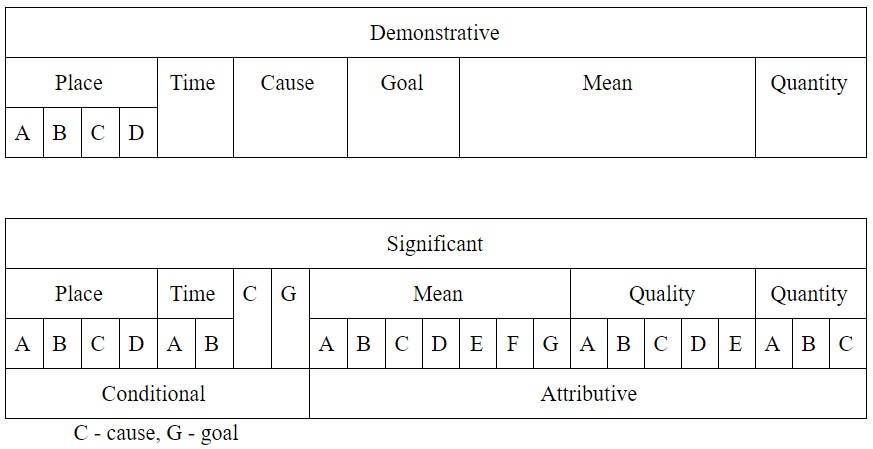
\includegraphics[width=\linewidth]{./sources/adverbs.jpg}
	\caption{Categories of adverbs}
	\label{fig:adverbs}
\end{figure}

\subsection{Demonstrative adverbs}

There are six categories of demonstrative\index{adverb!demonstrative} adverbs. They are adverbs of place, time. cause. goal, mean, quantity.

1. \textbf{Demonstrative adverbs of place.}

Let’s speak about subcategories of this adverbs. 

A. \textit{Adverbs indicating the place of action.}

Question: \textit{Where? (Kųde?)}

Here - \textit{Tut, zdě}

There - \textit{Tamo}

Everywhere - \textit{Vsëde, vsüdu, vsëkųde}

Nowhere - \textit{Nide, nikųde}

Somewhere - \textit{Něde, někųde}

B. \textit{Adverbs indicating the place where action is directed. }

Question: \textit{Whither? (Kųda?)}

Here

There

Everywhere

Nowhere

Somewhere


C. \textit{Adverbs indicating the place of action’s start.}

Question: \textit{Whence? (Odkųde?)}

Here

There

Everywhere

Nowhere

Somewhere


D. \textit{Adverbs indicating the place of action’s start.}

Question: \textit{Where? How far? (Dokųde?)}

(Up to) here

There

Everywhere

Nowhere

Somewhere


2. \textbf{Demonstrative adverbs of time}

Question: \textit{When? (Koĝda?)}

Now

Afterwards

Later

Then

Once

Sometimes

Ever

Never


3. \textbf{Demonstrative adverbs of cause}

Question: \textit{Why? (Čomu?)}

Therefore

Because

Thus

Somehow

Once


4. \textbf{Demonstrative adverbs of goal}

Question: \textit{For what? (Za čto?)}

For

In order to

So as to


5. \textbf{Demonstrative adverbs of mean}

Question: \textit{How? (Kako?)}

So

Likewise

Somehow

Otherwise

Nohow

Like that

That way

Anyhow

Differently


6.\textbf{ Demonstrative adverbs of quantity}

Question: \textit{How much? (Kolïko?)}

So much

Few

Some

Several

Nary


\subsection{Significant adverbs}

Significant\index{adverb!significant} adverbs are often divided into two large subcategories - conditional and attributive adverbs. \textit{Conditional} adverbs shows the conditions of the action took place - place, time, cause, goal. \textit{Attributive} shows the attributes of the action - the mean of the action. its quality and its quantity.

1. \textbf{Significant adverbs of place.}

A. \textit{Adverbs indicating the place of action.}

Question: \textit{Where? (Kųde?)}

Next to (close to)

Ahead

Opposite

Around

Far

Not far

Among

Between

At home

Upstairs

Downstairs


B. \textit{Adverbs indicating the place where action is directed. }

Question:\textit{ Whither? (Kųda?)}

Ahead

To the right

Upwards

Sideways

Downwards

Opposite

Home


C. \textit{Adverbs indicating the place of action’s start.}

Question: \textit{Whence? (Odkųde?)}

From upstairs

From downstairs

From the right

From the left


D. \textit{Adverbs indicating the place of action’s start.}

Question: \textit{Where? How far? (Dokųde?)}

(Up to) here

There

Everywhere

Nowhere

Somewhere


2. \textbf{Significant adverbs of time}

Question: \textit{When? (Koĝda?)}

Now

Afterwards

Later

Then

Once

Sometimes

Ever

Never


3. \textbf{Significant adverbs of cause}

Question: \textit{Why? (Čomu?)}

Therefore

Because

Thus

Somehow

Once


4. \textbf{Significant adverbs of goal}

Question: For what? (Za čto?)

For

In order to

So as to


Further let’s speak about attributive significant pronouns.

1. \textbf{Significant adverbs of mean}

Question: \textit{How? (Kako?)}

So

Likewise

Somehow

Otherwise

Nohow

Like that

That way

Anyhow

Differently

2. \textbf{Significant adverbs of quality}


3.\textbf{ Significant adverbs of quantity}

Question: \textit{How much? (Kolïko?)}

So much

Few

Some

Several

Nary

\subsection{Degrees of comparison}

Likewise adjectives, adverbs have three degrees of comparison\index{comparison}. Moreover, there are synthetic analytic forms too. 

Remember (look at paragraph about adjective degrees of comparison), that there ar three degrees: positive, comparative and superlative.

\textbf{Synthetic forms}

Comparative\index{comparison!synthetic} form is made by adding to the word base the suffix “ěǐ’. Unlike adjectives, this is the only suffix to create a comparative form (compare with suffixes “ëǐ”, “aǐ” for hard and soft bases in adjectives). 

\textbf{Examples:}

\textit{Mnogo - Množěǐ}

\textit{Sïnë - Sïněǐ}

Superlative form is made so as it is in adjectives - adding a suffix “naǐ-” to the comparative form.

\textbf{Analytic forms}

Analytic\index{comparison!analytic} forms provide simple ways of creating comparative and superlative forms without modifying the word itself. There two types of adverb analytic comparison.

\textbf{Using prefixes}

Comparative form is created by adding prefix “po-” through a defis ro a positive form. Superlative form is created by adding prefix “naǐ-” through a defis to the positive form.

\textbf{Examples:}

\textit{Mnogo - po-mnogo - naǐ-mnogo}

\textbf{Using an auxiliary adverb}

To the positive form you should add an auxiliary adverb in comparative or superlative form.

\begin{table}
	\begin{tabular}{lll}
		Auxiliary adverb
		& Comparative form
		& Superlative form \\
		more & bolěǐ & naǐbolěǐ \\
		less & mëněǐ & naǐmëněǐ \\
	\end{tabular}
\end{table}

\textbf{Examples:}

\textit{Mnogo - bolěǐ mnogo - naǐbolěǐ mnogo}

You can use synthetic and analytic forms at the same time.

\section{Predicative}

\begin{table}[!htb]
	\caption{Predicative characteristics}
	\begin{tabular}{ll}
		\textbf{Title}              & \textbf{Value}                            \\
		Semantic value              & Predicate                                 \\
		Category                    & Independent                               \\
		Subcategory                 & Nominal                                   \\
		Alteration                  & None                                      \\
		Alteration parameters       & None                                      \\
		Differentiation parameters  & Tense                                  
	\end{tabular}
\end{table}

Predicative\index{predicative} is a POS that is closely deriving to the predicate. Formally, it is an adverb that plays the role of the predicate (concluded in the predicate as a part of it). 

You should divide a syntax and morphological definitions of predicative. Now we are talking about the second one. In russian philology you can find the term of “condition category” - the equivalent for predicative (morphological definition). In this paragraph we will speak just about this term.

Predicative determines the class of words indicating an attribute or a condition of a person, environment etc., especially mental. Predicatives cannot be alternated, though they can be differentiated by tenses using an auxiliary verb “to be”. 

Predicatives have homonyms with adverbs, and nouns.  

\textbf{Examples:}

\textit{Ona hlådno mi kazala, če ne hoče da vidi mę} - She coldly said to me she does not want to see me (Adverb)

\textit{Dnësj je hlådno.} - It is cold today. (Predicative)

The most popular case of using predicative are modal constructions like "it is necessary", "it is needed" in passive form. Look at the following examples to compare active and passive forms.

\textit{Ja trěbam idati v còrkvu} - I should go to the church

\textit{Je nuđno mi da idam v còrkvu.} -  It is necessary for me to go to the church
\section{Verb}

Verb\index{verb} is a POS that describes the predicate and its properties. 


\subsection{Verbal types}

Learning Slavic languages you could mention that there is a set of verb suffixes that is very eliminated. Novoslovnica provides a theory that allows you to construct a right verb form.
Verbs with different verb suffixes represent different verbal types. There are four types of verbs in Novoslovnica.

\begin{itemize}
	\item A-type\index{verb!a-type}: verbs of this type define that the action in common sense.  
	\item E-type\index{verb!e-type}: verbs of this type define that the action is long-termed.
	\item I-type\index{verb!i-type}: verbs of this type define that the action is short-termed. This type comprises verbs with suffixes I and O. The suffix O is used when the consonant before the constructed suffix is involved in alterations depending on soft vowels that the vowel I is.
	\item U-type\index{verb!u-type}: verbs of this type define that the action is dotty.
	\item Extra type\index{verb!extra-type}. Is formed with the suffix “-OVA-” and defines the repeated action.  
\end{itemize}

When you speak about the action, you find what characteristic is suitable for the action and then use one of the predefined verbal types.

Somebody can ask what are the differences in tenses and types, because it might be confusing. However, verbal type determines the durability of the action (or its repeating property) while tense determines tense characteristic of the action such as completeness, stability in time, result, order etc.

All tenses provide difference between conjugation of different verbal types except imperfect. This tense has the common conjugation table for all verbal types. 

Further we will speak about conjugation itself. We will look at verb conjugation in indicative mood first of all. Then we will speak about other moods.

\subsection{Active voice}

Active\index{voice!active} voice shows that the person makes the action by himself. So, the subject of the sentence and the actor are the same.

\subsubsection{Indicative mood}

Verbs in indicative\index{mood!indicative} mood can be found in every tense that Novoslovnica possesses. Let us look at some tables with verb of different verbal types conjugation.

\subsubsection{Present Tenses}

There are two present tenses in Novoslovnica - Present Indefinite and Present Definite (see the chapter about tenses). In the appendix you can see the conjugations of five verbal types in Novoslovnica. The only exception is the verb "byti" that has a unique type of conjugation.

As you can see in the table 8.26 the verb "byti" has two forms - a full one and a short one. Usually, the full form is used separately without a NP with it. Using a subject with a verb leads to short form using. Look at the examples:

\textbf{Examples:}

Jesòm iz Moskvy - I am from Moscow (no pronoun)

Ja sòm iz Moskvy - I am from Moscow (with a pronoun) 

\subsubsection{Future Tenses}

\textbf{Future Definite Tense (Bųdešt čas)}

The Future Definite Tense is formed with the following:

\begin{itemize}
	\item Using HTE (3p. sg. of the verb "hteti" (to will)) + the verb in Present Definite or Indefinite Tense
	\item Using the future form of the verb "byti" + infinitive
	\item Using single-form conjugation 
\end{itemize}

The second variant semantically is close to English Future Continuous Tense. However, they both can be used to indicate the future action (see more details in the Tense section).

The verb "byti" also has a unique type of conjugation in Future Definite Tense.

\textbf{Pre-Future Tense}

This tense is form doubly: 

\begin{itemize}
	\item Using \textit{hte} with Perfect tense form of the main verb.
	\item Using the verb "byti" in pre-future form with the infinitive of the main verb.
\end{itemize}

The conjugation of the verb "byti" in pre-future tense you can find in the table in the appendix.

\textbf{Future Indefinite Tense}

Future Indefinite Tense is formed by \textit{hte} along with the Plusquamperfect main verb form.

\subsubsection{Past Tenses}

There are four past tenses in Novoslovnica (see the "tense" chapter). Though, only one of them distinguishes by verbal types (Aorist). Imperfect has a common conjugation for all verbal types while Perfect and Plusquamperfect have complex verb phrases.

The verb "byti" has also a separate declension in Aorist.

\subsubsection{Future-in-the-Past Tenses}

\textbf{Future-in-the-Past}

This tense is formed by the verb "hteti" in Imperfect with DA-form of the main verb.

\textbf{Pre-Future-in-the-Past}

This tense is formed by the verb "hteti" in Imperfect with perfect DA-form of the main verb.

\subsubsection{Declarative mood}

Declarative mood of the verb has all tenses existing in Indicative. It is formed using the verb "imati" (to have) with the corresponding passive participle of the main verb.

\subsubsection{Subjunctive mood}

Subjunctive\index{mood!subjunctive} mood shows two states of an actions. In the first state it can show a desirable action. In the second one it can show an action that has not become a real one. 

Subjunctive mood has only one-tense form. It is constructed with the verb “byti” in a subjunctive form with an aorist or imperfect participle. Special forms of the verb “byti” you can see in the next table.

\begin{table}[!htb]
	\begin{tabular}{llll}
		Subjunctive mood & Singular & Dual & Plural \\
		1 person & Bih & Bihma & Bihme \\
		2 person & Biša & Bihta & Bihte \\
		3 person & Biše & Biha & Bihu
	\end{tabular}
\end{table}

\subsubsection{Imperative mood}

Imperative\index{mood!imperative} mood shows that the actor make somebody do some action (imperate another object). Imperative mood also has only one tense to be used in. 

\subsubsection{Inferential mood}

Inferential\index{mood!inferential} mood is used when we speak about actions that we did not observe by ourselves. This mood mostly is used in tales, histories two show that we were not witnesses of what we are speaking about.

\newglossaryentry{ppp}{name=PPP, description={Past Passive Particle}}

Inferential mood is created by using the verb “ïmáti’ with the past passive participle (\gls{ppp}). This mood can be used in all tenses of the indicative mood (we should only place the verb “ïmáti” into this tense and add a PPP of the main verb to it). 

\textbf{Examples:}

\textit{Ja sòm rođen svojoǐ mamoǐ} - I am born by my own mother. (This is a real fact, but the actor (Mother) is not at the subject place in the sentence - Passive Voice).

\textit{Ona má rođeno ove rebętko.} - Some say she bore this child (This is a rumor, and the actor is in the place of a subject - Inferential mood of AV)

\subsection{Medial voice}

Medial voice has an equivalent amount of moods and tenses to be expressed with. The difference is in using the reflexive pronoun next to the word. Usually, the reflexive mark is placed right before the main verb in the verbal phrase.

Look at the example to see it:

\textit{Ja hoču \textbf{sę učiti} anĝliǐskomu jazyku} - I want to study English.

\textit{On hte \textbf{sę dojedna} do toga ruha} - He will join that movement.

\subsection{Passive voice}

\newglossaryentry{pv}{name=PV, description={Passive Voice}}

Passive\index{voice!passive} (\gls{pv}) voice shows that the person is an object for the action. That means, that the subject of the sentence semantically is not an actor, but the object. 

Passive voice has only two moods - Indicative and Subjunctive. Passive voice is created by using the verb “byti” with the \gls{ppp}. Here is the narrow border between Inferential mood of Active Voice and Indicative mood of Passive Voice.

We can describe the difference between these two terms in such a way. If we speak about real actions that we have imagined or we heard about them (however, the actor of these sentences is placed in the subject) - we use Inferential mood. And if we speak about any action that has no actor in the subject syntax role - we use Passive Voice. Let’s look at the examples.


\subsection{Infinitive and Supine}

Infinitive\index{infinitive} is a normal main form of the verb. In fact all languages that have an infinitive form of the verb use it in that way. So when you look through the dictionary looking for a verb, you should remember that it will stand in infinitive. Infinitive form is created by adding the ending “-ti” to the end of the verb. (Compare with English, you put the particle “to” before the verb to create the same form - there is some similarity in both cases). Infinitive has no parameters for declination.

Infinitive is a form to describe a verb as a process or an action itself.

The second unchangeable form of the verb is supine. It has no equivalent in English. Semantically, it is similar to the construction “to be going to do something”, determining the aims of the subject. Supine in Novoslovnica is built by adding the “-tj” ending to the end of the verb.

Supine\index{supine} had a great usage area in the past, now it is still used in Uppersorbian, Lowersorbian and Slovenian languages. It is mostly used with the verbs of motion, such as “to go”, “to swim”, “to move”, “to fly” etc.

\textbf{Examples:}

\textit{Ty hteš kazati mi něčto, da li?} - You want to say me something, don’t you? (Infinitive)

\textit{Mamo, ja idaju spatj dnesj po-rano.} - Mom, I’m going to sleep now earlier. (Supine)

\section{Transgressive}

Transgressive is a verbal independent POS, however some scientist suppose that it is only a form of a verb. so as infinitive and supine.
Transgressive cannot be declined, it has verbal characteristics (i.e. forms) but it is derived from participle with its suffixes. Let us look at the table with transgressive forms.

Imperfect form
Perfect form
Suffix
%-ја-(-чі-) || -јучі
%-в-(-шы)

We see that there are no endings here, that means transgressive cannot be declined. Perfect form determines the action that is completed (in past, present or future). Imperfect form determines the action is being done (in past, present or future). This fact differ transgressives from participles, because, as you can see, participles are divided by tenses, not by forms. However, transgressive is “over” the tenses. 

I should say that a consonant “j” in imperfect form transforms into a soft symbol after consonants. 

There are recommendation about using different forms of transgressive. Perfect forms with “-v-” are used when we speak about actions in the past (Aorist), while forms with “-všy-” are used when we speak about resultative action by the present moment (Perfect). Imperfect full forms with “-jačï-” are less preferred than with “-jučï-”. Moreover, these full forms are recommended to be used as a reflection of actions in the past (Imperfect), while short form of “-ja-” should be used as a reflection of actions in Present Concrete tense.

Transgressive can be replaced with a relative clause in the sentence with the relation “when”. Look at the examples:
% Казавшы му нѣчто, той изидаше из дома.
% Коґда той казал быше му нѣчто, он изидаше из дома.



\section{Participle}

\begin{table}[h]
	\caption{Adjective characteristics}
	\begin{tabular}{lllll}
		\textbf{Title}              & \textbf{Value}               \\
		Semantic value              & Attribute                    \\
		Category                    & Independent                  \\
		Subcategory                 & Verbal                       \\
		Alteration                  & Declension                   \\
		Alteration parameters       & Case, Number                 \\
		Differentiation parameters  & Type, Voice, Tense, Gender
	\end{tabular}
\end{table}

Participle is an independent verbal POS, that defines the action of another actor as its attribute. Participle is a POS between the nominal and verbal type, so as a pronoun, because it has properties of tense, voice, gender, case and number.

There are essential participles and auxiliary participles. The first ones can be used as attributes of nouns, they are far distanciated from the verb. They are Active and Passive Participles.

Auxiliary participles are quite closer to verbs, they participate in grammar constructions. They are Aorist and Imperfect participles.

Let us look at the tables to define how to use different participles.

A-type

\begin{table}
	\begin{tabular}{lll}
		& Present Tense & Past Tense \\
		 Active Voice & -ajučïǐ & -avšyǐ \\
		 Passive Voice & -ajemyǐ & -anyǐ/-enyǐ
	\end{tabular}
\end{table}

Aorist participle: Verb base + “-al”

Imperfect participle: Verb base + “-ěl”

E-type

\begin{table}
	\begin{tabular}{lll}
		& Present Tense & Past Tense \\
		Active Voice & -učïǐ & -evšyǐ \\
		Passive Voice & -ujemyǐ & -etyǐ
	\end{tabular}
\end{table}

Aorist participle: Verb base + “-el”

Imperfect participle: Verb base + “-ěl”

I-type

\begin{table}
	\begin{tabular}{lll}
		& Present Tense & Past Tense \\
		Active Voice & -ijučïǐ & -ivšyǐ \\
		Passive Voice & -imyǐ & -ityǐ
	\end{tabular}
\end{table}

Aorist participle: Verb base + “-il”

Imperfect participle: Verb base + “-ěl”

U-type

\begin{table}
	\begin{tabular}{lll}
		& Present Tense & Past Tense \\
		Active Voice & - & -nuvšyǐ \\
		Passive Voice & - & -nutyǐ
	\end{tabular}
\end{table}

Aorist participle: Verb base + “-nul”

Imperfect participle: None

Extra-type 

\begin{table}
	\begin{tabular}{lll}
		& Present Tense & Past Tense \\
		Active Voice & -ujučïǐ & -ovavšyǐ \\
		Passive Voice & -ujemyǐ & -ovanyǐ
	\end{tabular}
\end{table}

Aorist participle: Verb base + “-oval”

Imperfect participle: Verb base + “-ujěl”

\section{Gerund}

Gerund\index{gerund} is a form of a verb that determines the process of an action. That means it is not an independent POS, but has some features that do not allow us to include the description about gerund in the paragraph about verb.

Gerund is formed from the infinitive of a verb by reducing a “-ti” ending and adding a suffix “-n-” and an ending “-e-”. Gerunds are often created only from verbs of A-type. However, you can construct gerunds from verbs of other types. Look at the examples:

\textbf{Examples:}

\textit{Pisati} (verb) - pisane (gerund) - To write/Writing

\textit{Nositi} (verb) - nosine (gerund, bad form) - nošane (gerund, recommended form) - To wear/Wearing

\textit{Pěti} (verb) - Pěne (gerund, bad form) - pějane (gerund, recommended form) - To sing/singing

Unlike infinitive or supine, gerund can be declined, but only in the singular. This fact unites it with the nominal POS. Simply speaking, gerund declines so as soft neutral nouns do despite the nominal/accusative form of “e”.

\begin{table}
	\begin{tabular}{ll}
	Case & Ending \\
	Nominal & -e \\
	Genitive & -ä \\
	Partitive & -ü \\
	Dative & -ü \\
	Accusative & -e \\
	Instrumental & -ëm \\
	Prepositional & -ě \\
	Locative & -ü \\
	Vocative & no form
	\end{tabular}
\end{table}

Let us look at some examples:

\textbf{Examples:}

\textit{Ja dobro znam pisane} - (Accusative) I am good at writing

\textit{Vlådam dobro pisanëm} - (Instumentative) My writing is good.

\textit{Ja ne pravim grěšek v pisanü} - (Locative) I do not mistake while writing

\subsection{Gerund vs Verbal noun vs Infinitive}

All of these three POSes describe a process. However, they are different (Gerund, verb form and noun form) so it is necessary to define the properties of each other.

Verbal noun describes a process as an object. Often it corresponds with the result of the action (\textit{pisanije} - the result of writing). It has a role of Subject or Object.

Gerund describes a process as an action (\textit{pisane} - the process of writing something). It also has a role of Subject or Object.

Infinitive represents a process itself as a definitive normal form (pisati - to write). It is used mostly in complex verbal forms.

\textbf{Examples:}

\textit{Ove pisanije je mnogo lěpo} - It is a beautiful writing.

\textit{Pisane je mnogo trudno dlä menę} - Writing is very hard for me.

\textit{Hoču pisati knigu} - I want to write a book.

\subsection{Gerund vs Transgressive}

Both Transgressive and Gerund are described through an "-ing" form in English. Therefore, it should be useful to have some distinguising rules to classify the verb forms in Novoslovnica.

Transgressive and gerund have different syntax roles (look for them in the next chapter). The following table shows which roles they can have.

\begin{table}
	\begin{tabular}{lll}
		Role & Transgressive & Gerund \\
		Subject & - & + \\
		Object & - & + \\
		Modifier & + & - \\
	\end{tabular}
\end{table}

Thus, Transgressive has an attributive value describing a predicate with an additional action as its modifier. Gerund represents the process itself so it has a subjective value while describing a process.
\section{Transgressive}

Transgressive is a verbal independent POS, however some scientist suppose that it is only a form of a verb. so as infinitive and supine.
Transgressive cannot be declined, it has verbal characteristics (i.e. forms) but it is derived from participle with its suffixes. Let us look at the table with transgressive forms.

Imperfect form
Perfect form
Suffix
%-ја-(-чі-) || -јучі
%-в-(-шы)

We see that there are no endings here, that means transgressive cannot be declined. Perfect form determines the action that is completed (in past, present or future). Imperfect form determines the action is being done (in past, present or future). This fact differ transgressives from participles, because, as you can see, participles are divided by tenses, not by forms. However, transgressive is “over” the tenses. 

I should say that a consonant “j” in imperfect form transforms into a soft symbol after consonants. 

There are recommendation about using different forms of transgressive. Perfect forms with “-v-” are used when we speak about actions in the past (Aorist), while forms with “-všy-” are used when we speak about resultative action by the present moment (Perfect). Imperfect full forms with “-jačï-” are less preferred than with “-jučï-”. Moreover, these full forms are recommended to be used as a reflection of actions in the past (Imperfect), while short form of “-ja-” should be used as a reflection of actions in Present Concrete tense.

Transgressive can be replaced with a relative clause in the sentence with the relation “when”. Look at the examples:
% Казавшы му нѣчто, той изидаше из дома.
% Коґда той казал быше му нѣчто, он изидаше из дома.
\subsection{Verbal Noun}

Verbal Noun\index{noun!verbal} is a group of nouns that were created from the verbs or their forms. Verbal forms can be formed twice: directly from the verb (from infinitive) and indirectly from gerund.

Direct verbal nouns are formed by reducing verb with its ending “-ti” and then adding some needed suffixes and endings.

There are two different means of forming a verbal noun such a way.

\begin{itemize}
	\item Adding suffix “-k-” or "-b-" and “-a” ending. The latter fact means that all these nouns are of the first type of declension. 
	\item Reducing verbal suffix (“-a-”,  “-e-” etc.) and adding null-ending. These nouns will be of the second declension.
\end{itemize}

Usually, the second mean corelates with English short nouns derived from verbs (to run - run, to breathe - breath etc.)

\textbf{Examples:}

\textit{Běg} - Run

\textit{Dyh} - Breath

\textit{Stroǐka} - Building

\textit{Myǐka} - Washing

\textit{Borba} - Struggle 

\textit{Sųdba} - Fate

However, not all verbs allow to create verbal nouns in such ways. So there is a better way of creating verbal nouns indirectly.

Indirect verbal nouns are formed by adding a suffix “-iǐ-” to the gerund. These nouns are of the second declension with “-je” ending. Remember the fact that before the vowel “-ǐ-” transforms into “-j-”. 

You can use the second type everywhere in your sentences. Nevertheless, if there is a verbal noun of the first type within the word lexeme, the verbal noun of the first type is preferred to be used.

Let us see the \textbf{examples}:

\textit{Pisati} (verb) - pisane (gerund) - pisanije (verbal noun)

\textit{Strojati} (verb) - \textit{strojka} (verbal noun, I type (preferred)) - \textit{strojane} (gerund) - \textit{strojanije} (verbal noun, II type (is not preferred))

\textit{Běgati} (verb) - \textit{běg} (verbal noun, I type (preferred)) - \textit{běgane} (gerund) - \textit{běganije} (verbal noun, II type (is not preferred))  


\section{Article}

If you tried to learn a Slavic language, you would notice that there is no articles. The term of definiteness is ruled mostly by demonstrative pronouns. However, there are two Slavic languages that provide this possibility - Bulgarian and Macedonian: these are Slavic analytic marvel (a pair of languages, that has worked out an completely different model of grammar). Novoslovnica let you use this achievement. So, now there is a question: what do articles in Novoslovnica look like and what are the differences between English articles?

Firstly, you should remember that there is no indefinite article. The word itself shows that you are speaking about a designatum and there is no concrete information about it, no details. However, if you want to accentuate the term of indefiniteness you can use an indefinite pronoun before the word (“Někyǐ”, “Něktoryǐ”).

Secondly, there are huge differences between definite articles in English and in Novoslovnica. English has only one article - “the”. It shows only the term of definiteness. Novoslovnica provides in articles additional meanings, which you have already seen in the paragraph about demonstrative pronouns - distance and visibility of the object. So, there are three definite articles in Novoslovnica: “-òt”, “-òn”, “-òv”. Also you should know that these articles have the differentiation by gender and number. 

òt – ta – to – te
òv – va – vo – ve
òn – na – no – ne

Despite other POS articles have only two number and alternate by gender only in singular. Words in dual rule the article in plural. I will remind you, that the article “òv” is used, when the object is in the field of view and it is rather close to you. The article “òn” is used, when you still see the object, but it is rather far from you. The article “òt” is used, when you cannot see the object or it is abstract, however you are talking about the definite instance of the designatum.

Finally, there are differences in the way to use the article. In English you place the article just before the word, dividing the word and the article by the space (different words). In Novoslovnica you put the article just after the word, dividing the word and the article by the hyphen (one word).

Examples: 


Articles in Novoslovnica, so as in English, have been derived from demonstrative pronouns (“tyǐ”, “ovyǐ”, “onyǐ”). Nonetheless, you can see that the pronoun “sïǐ” has not developed into the article.

\section{Particle}

Particle\index{particle} is a dependent part of word. Particles add an auxiliary meaning to the main word. There are some groups of particles.

Positive

* Aga - Yeap

* Ugu - Yeah

* Da - Yes

Negative

* Ne - Not
* Ni...ni - Neither...nor

Interrogative

* Či - Whether

* Li - Whether

Estimative

* Kakto - Like

* Mòl - Supposedly

Comparative

Incentive

Exclamative

Amplificative


Specifying

Restrictive

Demonstrative



\section{Preposition}

Prepositions\index{preposition} also are not an independent POS. They are closely related to the main word (often it is a noun). Most prepositions show the direction or the location of the action. 

We can divide prepositions into two main groups, so as we did with adverbs. We can distinguish \textit{primary} and \textit{secondary} prepositions. Primary prepositions are very ancient and we cannot refer to any word form they have formed from. Secondary prepositions are longer, and they appeared by semantic shift of an adverb, transgressive or a cased-noun. 

Here I will list primary prepositions with English translations and controlled cases. Complex cases are commented in notes.

\textit{Bez} (Gen.) - Without

\textit{V} (Acc.) - In, into

\textit{Dlä} (Gen) - For

\textit{Do} (Gen.) - To

\textit{Za} (Instr.) - For

\textit{Iz} (Gen.) - From (inside the object)

\textit{K} (Dat.) - To

\textit{Krôz} (Skrôz) (Gen.) - Through

\textit{Na} (Acc.) - On

\textit{Nad} (Instr.) - Above

\textit{O} (Prep.) - About

\textit{Od} (Gen.) - From (the object)

\textit{Po} (Dat.) - Along

\textit{Pod} (Instr.) - Under

\textit{Pri} (Loc.) - At

\textit{Pro} (Acc.) - About (the difference between “O” and “Pro” is in the detail view on the object. When we say the second variant we just mention the object in our speech, while using the first one we talk about it in details).

\textit{S} (Instr.) - With

\textit{U} (Gen.) - At (the difference between “Pri” and “U” is in the object of speaking. When we use “U” we mention real object in space and place the object of speaking near it. “Pri” is used when we speak about proximity in time, i.e. some events are close to each other.)

\textit{Črez} (Acc.) - After,  in (time)

The following figure shows the semantics of most primary prepositions.

\begin{figure}
	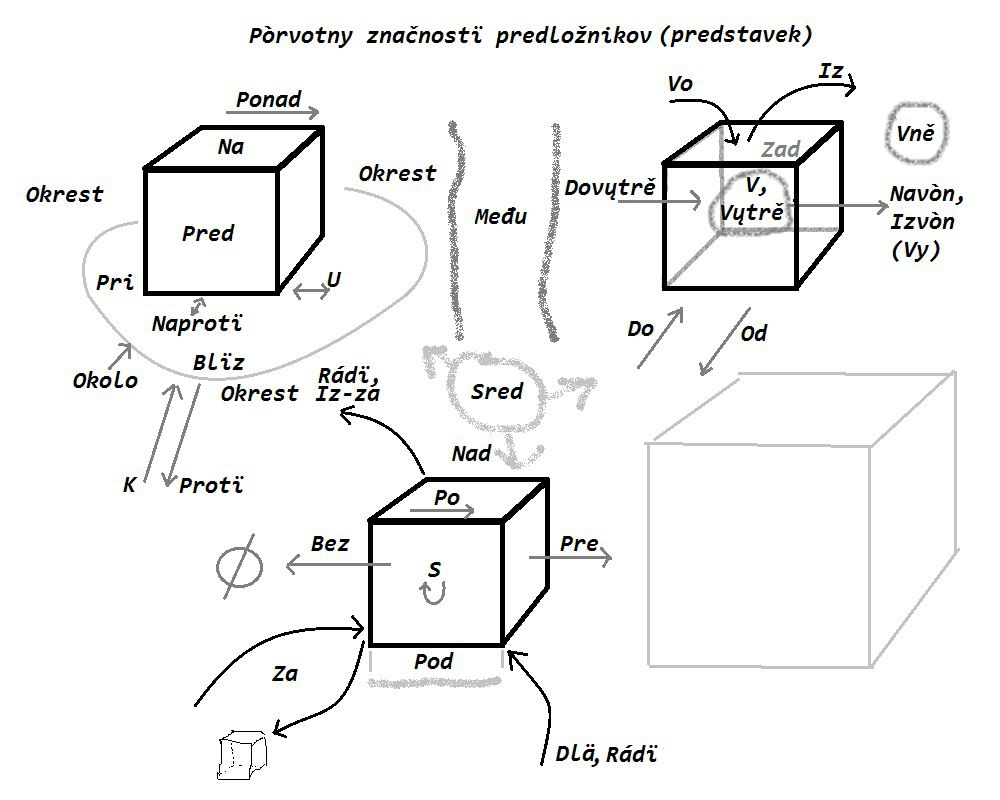
\includegraphics[width=\linewidth]{./sources/prepositions.jpeg}
	\caption{Prepositions in Novoslovnica}
	\label{fig:prepositions}
\end{figure}

Secondary prepositions are derived from nouns or adverbs with the shift of semantic from independent to an auxiliary one. For examples, preposition "Pred" is derived from the noun "Pred" (Front). Using separately in refers to a frontal part of something. Using with an additional independent word it becomes a preposition defining the frontal part of the word that follows it.

\textbf{Examples:}

\textit{Svòrh} - Over

\textit{Među} - Between
\section{Conjunction}

You see that there is a rather big amount of prepositions on Novoslovnica. However, the amount of conjunctions\index{conjunction} is much smaller. 

Conjunctions are divided into two classes: \textit{coordinating} and \textit{subordinating} conjunctions.

Coordinating\index{conjunction!coordinating} conjunctions usually connect sentence elements of the same grammatical class (N + N, V + V etc.). Syntactically, coordinating conjunctions connect either homogenuous sentense parts or independent clauses in a compound sentense. There are four kinds of coordinating conjunctions: copulative, adversative, disjunctive and illative.

\textbf{Conjunctive}:

I - and

Da - and

Ta - and

Ili - or

Či - or

Abo -or

\textbf{Adversative}:

Ale - but

Ama - but

No - but

Jednako - but

\textbf{Disjunctive}

Alïbo - either ... or

Lïbo - either ... or

A - and

\textbf{Illative}

Bo - because, that is why

Tako - thus, so

Subordinating\index{conjunction!subordinating} conjunctions are used to connect clauses in subordinate sentence. They complement the functionality of corresponding adverbs.

\textbf{Subordinative}:

Dabi - for

Aby - for

Da - for

This is the whole list of conjunctions existing in Novoslovnica today.

\section{Interjection}

This interesting POS is used to describe emotions within the sentence. Interjections\index{interjection} are neither independent nor dependent POS. They even are not involved into sentence structure. They just show the color of the sentence to let the interlocutor understand your feelings. 

Interjection is a POS that has no semantic meanings. Interjections are not words in our common comprehension. They are sounds that we produce. Sometimes it is rather difficult to say what differences are between interjections and senseless sounds that we can produce (i.e. some spontaneous exclaims, murmuring etc.). Interjections are divided into intended exclaims (with bright emotional color) and sound imitations (i.e. animal voices imitation) that are united in Novoslovnica within the POS of Onomatopoetics. So, Interjections in Novoslovnica are only used to express emotional exclaims.

Interjections are divided into three groups depending on their aim: emotional, imperative and etiquette. 

\textbf{Emotional interjections}

Emotional interjections can be divided into negative and positive interjections.

Positive:

Ah - Ah

Ŭaŭ - Wow

Ŭah - Wow

Ura - Hurray

Ogo - Wow

Uf - 

\textbf{Negative}

Oh - Oh

O-o - Oh

Be - 

Hehe -

Heh -  

Éh - 

Jo - 

Fu - 

\textbf{Ambiguous} (depend on the context):

Uh - Uh

Oǐ - Oh

Aǐ - 

Išty - 

Hm - Hmm

\textbf{Imperative interjections}

Let us look at them:

Éǐ - Hey

Na - Take it

Stop - Stop

Bre - Man

A-u - 

Allo - Hello

Brysj - Go out

Von - Out

\textbf{Etiquette interjections}

These interjections are often whole words, that we use without the sentence context in some situations that need our etiquette.

Hvála - Thanks

Dobrodošli - Welcome

Dękujem - Thanks

Zdråveǐ - Hi

Zdråveǐte - Hello

\section{Onomatopoetic words}



\chapter{Phrase}

\section{Collocation}

A \textit{collocation} is an expression consisting of two or more words, that the one is main and the other are subordinative. Usually, collocation consists from 2 to 5 words. Subornative words are connected to the main one by several types of links: coherence, management and adjunction.

\textbf{Coherence} between the main and the subordinative words lies in corellation of grammar forms. That means the subordinative word should correspond with the main one while the latter changes (i.e. case or gender). Thus, coherent link introduces a strong connection between the two words, so they change both when a primary link is established and when the word changes (declension or conjugation).

\textbf{Examples:}

- \textit{Lěpa žena - Lěpu ženu - Lěpoǐ ženě} (Beautiful woman in Nominative, Accusative and Dative)

- \textit{Sïlen věter - Sïlnoga větra - Sïlnomu větru} (Strong wind in Nominative, Genitive and Dative)

\textbf{Management} link has a weaker connection between the words. The word with a management link has a determined grammar form. So the subordinative word should be changed once when is connected to the main word and then it is not changed while the main word is declining or conjugating. The primary word form is managed by the main word within a rule-case. It can be of a determined case or a preposition to be used with.

\textbf{Examples:}

- \textit{Věnec života - Věnca života - Věncom života} (The culmination of life in Nominative, Genitive and Dative)

- \textit{Kniga o važlivom - Knigy o važlivom - V knigji o važlivom} (A book of something important in Nominative, Genitive and Locative)

\textbf{Adjunction} means we simply add a subordinative word to the main one to form a collocation. We usually speak about this type while linking when we have immutable words.

Examples:

- \textit{Glųboko spati} (To have a deep sleep)

- \textit{Hoditi dalïko} (To walk far away)

Using proper cases in a collocation has a great importance for constructing an euphonious and understandable sentence. However, we cannot define all the cases of such links now, so you can feel-in the language to achieve this. If you are Slavic, simply try to use those cases or constructions that you use in your native language. If you are not, try to use English logic that is sometimes close to Novoslovnica, in a number of cases.
\section{Emphasis}

Emphasis is a logical accent in a phrase. Often we allocate the accented words with the voice while speaking, but sometimes we need to show the accent in writing or strongify it. So here you can take a look at tools of showing the accent in your phrase.

The most suitable way of it is to use particles “že”, “ž”, “pretož”, “vědj”. The accent depends on place where the particle stands in your sentence. 

\begin{itemize}
	\item In the beginning - this makes the accent on the first word in a phrase (sentence)
	\item After the first word - this makes the accent on the whole phrase (sentence)
	\item After the second … last word - this makes the accent on the second … last word in your phrase (sentence)
\end{itemize}

Examples:

\section{Phraseology}

Ja mám něčto - Něčto je u menę

There are two constructions that we can use to describe an English variant “I have something”.
As you see, the exact translation of the English phrase is the first variant. Here we use the verb “máti” (to have). However, there is the second variant in Novoslovnica too. In this variant we can watch the interchange between the actor and the object of an action by syntax roles. In “Ja mám něčto” we see that the actor is the subject of this short sentence, and the action object is has a syntax role as a direct object. In “Něčto je u menę” we see, that the actor has a role of indirect object and the object has a subject syntax role.    

There are some connections between the second variant of the phrase and the English “There is/are” construction. In English we use this when the object is situated in some place, so as in the second variant (if we change the actor (indirect object) with the adverbial (or indirect object of location). In Novoslovnica we still can use this construction with the soulful objects such as personal pronouns or animated nouns. 

Jesòm někto - Jesòm někym

You can notice that there are different construction of translation a phrase “to be somebody” in Novoslovnica. These two variants, with normal form and Instrumentative, are equal. 
The accent of using these two forms lays in the linguistic formalism that you use in your speech. Using a normal form instance of cases (Remember, that you cannot use Nominative itself in the non-Subject roles in your sentence) is more analytic while using Instrumentative is more synthetic.
Nevertheless, they both can be used in speech.

\chapter{Syntax}

\section{Clause}

A clause is the smallest grammatical unit that represents a complete proposition. An ordinary clause consists of a NP and VP.

NP, or Noun (Nominal) Phrase, is a construction into which nouns most commonly enter, and of which they are the head word. \cite{lang-dict}

VP, or Verb Phrase, has two senses \cite{lang-dict}. 

The term verb phrase is used in two senses. Traditionally, it refers to a group
of verbs which together have the same syntactic function as a single verb,
e.g. is coming, may be coming, get up to. In such phrases (verbal groups, verbal
clusters), one verb is the main verb (a lexical verb) and the others are subordinate to it (auxiliary verbs, catenative verbs). A verb followed by a non-verbal
particle (similar in form to a preposition or adverb) is generally referred to as
a phrasal verb.
In generative grammar, the verb phrase (VP) has a much broader definition,
being equivalent to the whole of the predicate of a sentence, as is clear from the
expansion of S as NP+VP in phrase-structure grammar. In the minimalist
programme, the head of the upper vp shell is referred to as little v.

a subject and a predicate, sometimes with additional auxiliary members. Predicate usually is composed of a verb with adverbial modifiers.

The subject determines the concept which is the actor in the sentence and the predicate determines the action which the actor is connected with.





% http://www2.ivcc.edu/rambo/eng1001/sentences.htm
% https://www.lexico.com/en/grammar/clauses

\section{Simple sentense}

Originally, a simple sentence consists of a single independent clause with a finite verb in it. Complex and compound sentences (look further) may be of multiple clauses, though a simple sentence has the only one.

\subsection{Subject}
The actor, that subject is indeed, can be described by different means. However, the most frequently used one is a noun. Every POS that is a subject in the sentence should be put into initial form. For a noun, its initial form is Nominative case. Noun in other cases cannot play the role of a subject.
Frankly speaking, a lot of POS in proper cases can play role of a subject. Now I want to list the most popular ones to let you know what is the point.

% Table

The most popular ones are first three rows.

At the end I will list the examples that could help you in understanding of how to put the word into its initial form to let it be the subject of a sentence. 

\textbf{Examples:}


\subsection{Predicate}
The action, which is provided by the actor, can be also described in different ways. The most popular is the verb, of course. The verb, determining the tense of the action, the person that does this action, the mood of the action, can be formed into every available for a verb form… Novoslovnica does not provide a noun being as a predicate (as it is available in Russian). Such sentences are transformed into the ones with the auxiliary verb “to be” as connection between the term and the determining word. 

\subsection{Auxiliary members}
The subject and the predicate are the main members of a simple sentence. However, you can notice that they do not provide  enough information to the interlocutor. That is why there are auxiliary members of a sentence, that give us necessary information.

\subsubsection{Object}
This auxiliary member gives the information about objects that are influenced by the action actor does. 
Here we should speak about one more classification of verb: by the mean of transitivity.

The transitive verb can have an object in accusative case without any prepositions.

The intransitive verb can have no objects or only with a preposition. 

\subsubsection{Adverbial}
Adverbial helps us to get some more information about predicate. Sometimes, they are involved in semantic connection with the verb and become actants. 

\subsubsection{Modifier}
Modifier brings some additional information about attributes of the subject, objects etc. They help us to build the exact picture of the situation that is described by a predicate.

\subsection{Word order}
There are languages with free word order and with strict one. Novoslovnica is a language with a declared word order, when changing the order of the words shifts a semantic value of the whole sentence. However, you can change some words in the sentences as you like. Let us see what the order is.

The common structure of simple sentence with neutral semantic value is SVO: \textit{Subject + Verb + Object}. From this thesis we can write down two rules:

Predicate is placed after the Subject

Object is placed after the Predicate it is connected to.

These rules are main if you want to create a grammatically proper sentence with neutral semantic value. 

There are also three additional rules:

\begin{itemize}
	\item Consistent grammar modifiers should be placed before the modified word.
	\item Inconsistent grammar modifiers should be placed after the modified word.
	\item Adverbials should be placed after the Predicate.
	\item Interrogatives should be placed at the beginning of the sentence.
\end{itemize}

These six rules can help you to understand what order is suitable for a Slavic sentence. There are also some constraints of what should not appear in your sentence:

\begin{itemize}
	\item Participial should be placed after or before the modified word.
	\item The particle “b/by” should not be placed in the beginning of the sentence.
\end{itemize}

Thus, now you are able to create a normal simple sentence with neutral semantic value. Nevertheless, you can gain a certain accent on the word you want by replacing words within the sentence.

Using SOV idiom you put the accent on the Object. 

Using VSO idiom you put the accent on the Verb (the Predicate)

Using OVS idiom you put the accent on the pair of Object and Predicate.

Using OSV idiom you put the accent on the pair of Object and Subject.

Using VOS idiom is equal to using a VSO idiom.

The same thing is about auxiliary members of the sentence - if you want to put an accent on the word, you should place it at the beginning of the sentence. Subject is an exception - its normal place is first, so you can put an accent on it only in your pronunciation.

\subsection{Incomplete sentence}
However, sometimes we do not need to say everything in our sentence, because it will cause tautology. Then we reduce some words calling for ellipsis. A sentence is named incomplete, when the subject or the predicate is not used in it.

\subsection{Substantive sentence}
Sometimes it is enough to say only a collocation or even the only word to show your idea to the interlocutor. This is what the substantive sentence is like.

We would not speak about them, because we suppose everything is quite clear. Just use phrases or the only word to express your idea.

\subsection{Relative clause}
Relative clause is one of grammar modifiers. It is a separate definition or adverbial, which has turned into a sentence that depends on the main one.

\section{Compound Sentence}

A compound sentence refers to a sentence that consists of two (or more) independent clauses in it. There are connected to one another with \textit{coordinating} link.

Coordinating sentences describe the relationship between the clauses with no dependency in it. Coordinating sentences are divided into three categories: \textit{copulative}, \textit{adversative} and \textit{consecutive}. These types of sentences are connected with the so-called types of conjunctions or adverbs. The exception is consecutive sentences where no auxiliary word is used.
 
Following examples shows the usage of coordinate sentences:

Examples:



\section{Complex Sentence}

A complex sentence refers to a sentence that consists of one (or more) dependent clauses connected to the single main one.

A dependent clause alone cannot stand for a complete sentence. The only way to form a complete one is to be connected to an independent clause and to form a complex sentence. Independent clauses are connected to the independent one with subordinate, conditional or relative conjunctions.

Thus, subordinating sentences are used to describe a relationship between parts with a dependency from one main clause (superordinate) to other subordinate.

Examples:

A conditional sentence describes something that is possible or probable.

Examples:

A relative clause is used for description of a part of the main clause.

The dependent clauses can go first followed by the independent one, and conversely.


\section{Reported speech}

There are some ways of describing person’s speech in the sentence. The first way is to use direct\index{speech!direct} speech. Look at the examples:

\textit{I say: “We need to go to the theatre”.} - (in quotes is situated my own phrase about going to the theatre)

\textit{- Come on, we need to go!, - exclaimed his brother.} - (after the hyphen we see a phrase of somebody’s brother).

Another way is to use a reported speech\index{speech!reported} - a way of describing what somebody has said without using of quotes. Look at the examples of reported speech in English.

\textit{He says (that) we’re going to stay here today.} (We just mention what HE says to us).

\textit{I said that we had finished this work the day before.} (I mention my words that I said previously without exact reproducing of them).

Reported speech is used when we refer to somebody’s words in our sentence implicitly. It is constructed with the ordinary sentence describing real situation and then a relative cause of a reported speech with reference to another expression, which is connected to the main clause with the relative pronoun or a subordinative conjunction.

However, like English, Novoslovnica has a tense-shift in using reported speech. You can see how the tenses shift in Indicative in the next table:

\begin{table}
	\begin{tabular}{ll}
		Tense in Direct Speech & Tense in Reported Speech \\
		Present Common & Present Common/Aorist \\
		Present Concrete & Aorist/Imperfect \\
		Future I & Future-in-the-Past I \\
		Future II & Future-in-the-Past II \\
		Future-in-the-Past I & Future-in-the-Past I \\
		Future-in-the-Past II & Future-in-the-Past II \\
		Aorist & Plusquamperfect (aorist part.) \\
		Imperfect & Plusquamperfect (imperfect part.) \\
		Perfect & Plusquamperfect \\
		Plusquamperfect & Plusquamperfect 
	\end{tabular}
\end{table}


\underline{Subjunctive}\index{mood!subjunctive} mood is reproduced in reported speech so as it is written in the direct one. 

\textbf{Examples:}

\textit{On kazal mamě, če ja bih htěl byti vozarom} - He told my mother that I would like to be a driver.

\textit{On je kazal, če htěl biše dojěhati do Gimalaja.} - He said he would like to get to Himalayas.

\textit{Môǐ prijatelj govorěh, če biše izučil vsï eŭropsky jazycy.} - My friend said he would learn all European languages.

\underline{Imperative}\index{mood!imperative} mood is reproduced in reported speech with using modal verbs and subjunctive mood of the main verb.

\textbf{Examples:}

\textit{Brat mi je kazal, če trěbam bih sgotvil oběd dnësj.} - My brother said I should prepare a dinner today.

\textit{Učitelj mi ukazaše mi že musim bih stvoril vsï děly.} - My teacher told me I must do all homework.

Declarative\index{mood!declarative} mood can be reproduced in reported speech doubly:

\begin{itemize}
	\item with using modal analogs of the English verb “might” with a tense-shifted verb in Indicative mood
	\item the verb in Inferential mood itself can be tense-shifted (we shift the tense of the auxiliary verb “ïmáti”).
\end{itemize}

\underline{Inferential} mood is already a type of reported speech, so it does not shift while using reported speech.

\chapter{Semantics}

There are three main parts of the sentence analysis that lead us to understanding: grammar, syntax and semantics. First two chapters were reviewed on the previous pages of the book. Here we are going to talk about the third main part of the linguistic analysis - Semantics.

We are not talking here about how to produce something like machine-assisted translator of Novoslovnica. However, we will consider some facts, that could help to deal with it. 

This chapter comprises three parts: the semantics of prefixes, the semantics of suffixes and common semantics that will describe the sense of roots and dependent \gls{pos}.

\section{Prefix}

\newglossaryentry{pow}{name=POW, description={Part of word}}
\newglossaryentry{prep}{name=PREP, description={Preposition}}

Prefix\index{prefix} is a part of a word (\gls{pow}) that stands before the word stem. One word may have more than one prefix. In other words, prefixes can be added one by one right to the beginning of the stem. Each prefix has its own semantic value and word changes its meaning due to the presence of exact prefixes.

We can divide prefixes into several groups. 

\begin{itemize}
	\item Borrowed - prefixes that were borrowed from other languages (i.e. Latin, English etc.)
	\item Native - Slavic prefixes, that have a clear semantic value
\end{itemize}

Novoslovnica possesses 35 native\index{prefix!native} and 9 borrowed\index{prefix!borrowed} prefixes.

Native: bez, v, vně, vųtrě, voz, vy, do, za, zad, iz, k, kų, među, na, nad, naǐ, ne, ni, o, od, pa, po, pod, poslě, pra, pre, pred, prez, pri, pro, råz, s, sô, u, črez.

Borrowed: a, antï, aŭto, kŭazï, mono, multï, pan, para, super

The chapter is to discuss the main prefixes, giving each of them a description and examples. Also one should consider that major part of prefixes are deeply connected with the prepositions. That means many prefixes can be used separately from the stem in a prepositional role. Such prefixes are marked with the PREP label. 

\textbf{Bez} \gls{prep}

Meaning: “without”

This prefix is an equivalent of the word “without” in English. It means the absence of something that we mention. As a prefix, it has no equivalence in English. Nevertheless, the suffix “-less” has a very similar meaning. Look at the example to get it.

\underline{Examples:}

\textit{Bez doma} - Without home

\textit{Bezdušen} - Without soul/Soulless 


\textbf{V} \gls{prep}

Meaning: “into” (direction or placement)

This prefix has a semantic value of “leading into something”. The preposition equals to “in” or “into” in English.

\underline{Examples:}

\textit{V búdji }- In the building

\textit{Vhoditi} - Enter

\textbf{Vně} \gls{prep}

Meaning: “outside” (placement)

\underline{Examples:}

\textit{Vně trudnostëǐ} - Out of problems

\textit{Vněrečen} - Outspoken

\textbf{Vųtrě}

Meaning: “inside” (placement)

\underline{Examples:}

\textit{Vųtrě dušy} - Inside a soul

\textit{Vųtrěseben} - Thoughtful

\textbf{Voz}

Meaning: “upside” (direction)

\underline{Examples:}

\textit{Vozmožen} - Possible

\textit{Vozběg} - Take-off

\textbf{Vy}

Meaning: “outside” (direction)

This one means “leading outside something”. The prefix has no prepositional equivalent, remember word “Vy” means “You”.

\underline{Examples:}

\textit{Vyhod} - Exit

\textit{Vyglěd} - Outlook

\textbf{Do} \gls{prep}

Meaning: “to” (destination)

This prefix shows the destination of a process to some point. In English we can find an equivalent “to”.

\underline{Examples:}

\textit{Idati do stěny }- go to the wall

\textit{Dodati} - add (something we give to a set of something to increase its amount or capacity)

\textbf{Za} \gls{prep}

Meaning: “for” (aim)

The semantic value of this prefix is the aim of an action. We use it when we want to reach something, some object. English “for” can be found as revealing one of its semantic values in equal way. 

\underline{Examples:}

\textit{Idati za cělïü} - go for the goal

\textit{Zavariti čaǐ }- To brew tea (in order to make it hot)


\textbf{Zad} \gls{prep}

Meaning: “behind, after” (follow)

This prefix has an artificial origin (This semantic value was divided from the previous prefix). It means placing an object behind another one. The equivalent is “behind”.

\underline{Examples:}

Bez doma - Without home
Bezdušen - Without soul/Soulless 

\textbf{Iz} \gls{prep}

Meaning: “from”

This prefix equals the English word “from”. 

\underline{Examples:}

\textit{Jesòm iz Moskvy} - I am from Moscow

\textit{Izhodnyǐ} - basic (from that we can develop something new)

\textbf{K} \gls{prep}

Meaning: “to” (direction)

\underline{Examples:}

Bez doma - Without home
Bezdušen - Without soul/Soulless 

\textbf{Kų}

Meaning: “what”

\underline{Examples:}

\textit{Kųda} - Where (What direction)

\textit{Kųdy} - When (What time) 

\textbf{Na} \gls{prep}

Meaning: “on” (placement)

Examples:
Bez doma - Without home
Bezdušen - Without soul/Soulless 

\textbf{Nad} \gls{prep}

Meaning: “above” (placement)”

Examples:
Bez doma - Without home
Bezdušen - Without soul/Soulless 

\textbf{Naǐ}

Meaning: “the most”

Examples:
Bez doma - Without home
Bezdušen - Without soul/Soulless 


\textbf{Ne} \gls{prep}

Meaning: “not”

Examples:
Bez doma - Without home
Bezdušen - Without soul/Soulless 

\textbf{Ni} \gls{prep}

Meaning: “even this/so”

Examples:
Bez doma - Without home
Bezdušen - Without soul/Soulless 

\textbf{O}  \gls{prep}

Meaning: “about”

Examples:
Bez doma - Without home
Bezdušen - Without soul/Soulless 

\textbf{Od} \gls{prep}

Meaning: “from” (direction)

Examples:
Bez doma - Without home
Bezdušen - Without soul/Soulless 

\textbf{Pa}

Meaning: “not real”

Examples:
Bez doma - Without home
Bezdušen - Without soul/Soulless 


\textbf{Po} \gls{prep}

Meaning: “along” (direction)

Examples:
Bez doma - Without home
Bezdušen - Without soul/Soulless 

\textbf{Pod} \gls{prep}

Meaning: “under” (placement)

Examples:
Bez doma - Without home
Bezdušen - Without soul/Soulless 

\textbf{Pra}

Meaning: “grand”

Examples:
Bez doma - Without home
Bezdušen - Without soul/Soulless 

\textbf{Pre}

Meaning: “more than”

Examples:
Bez doma - Without home
Bezdušen - Without soul/Soulless 

\textbf{Pred} \gls{prep}

Meaning: “before, in front of” (placement)

Examples:
Bez doma - Without home
Bezdušen - Without soul/Soulless 

\textbf{Prez} \gls{prep}

Meaning: “rapidly through”

Examples:
Bez doma - Without home
Bezdušen - Without soul/Soulless 


\textbf{Pri} \gls{prep}

Meaning: “close to, approach” (direction)

Examples:
Bez doma - Without home
Bezdušen - Without soul/Soulless 

\textbf{Pro} \gls{prep}

Meaning: “rapidly through”

Examples:
Bez doma - Without home
Bezdušen - Without soul/Soulless 

\textbf{Råz}

Meaning: “different”

Examples:
Bez doma - Without home
Bezdušen - Without soul/Soulless 

\textbf{S} \gls{prep}

Meaning: “with”

Examples:
Bez doma - Without home
Bezdušen - Without soul/Soulless 

\textbf{Sô}

Meaning: “alongside”

Examples:
Bez doma - Without home
Bezdušen - Without soul/Soulless 

\textbf{U} \gls{prep}

Meaning: “near”

Examples:
Bez doma - Without home
Bezdušen - Without soul/Soulless 

\textbf{Črez} \gls{prep}

Meaning: “slowly through”:

Examples:
Bez doma - Without home
Bezdušen - Without soul/Soulless 


\section{Suffix}

Suffix - is a \gls{pow}, that is placed after the word stem. It is a postfix that is not an ending of the word. That means that added a suffix to the word makes a new one with its own semantic value. Here is the list of main suffixes in Novoslovnica with their semantic value and examples.

\textbf{Ak}

This suffix has a semantic value of “person of some quality”.

\underline{Examples:}

\textit{Bědnäk - Běden (adj)} - Poor man - Poor (adj)

\textit{Glupak - Glup (adj)} - Fool - fool (adj)

\textbf{An}

This suffix has a semantic value of “having some property”.

\underline{Examples:}

\textit{Ušan - Uho (noun)} - Plecotus - Ear (noun)

\textit{Leganka - Legati (verb)} - Bed - to lie (verb)

\textbf{Ar}

This suffix has a semantic value of “person of some profession”. The suffix has a similar meaning with English "-er".

\underline{Examples:}

\textit{Rybar} - Fisher

\textit{Ovčar} - Shepherd

\textit{Ač}

This suffix has a value of "person that likes to perform an action"

\underline{Examples:}

\textit{Grač - Grati} - Player - To play

\textit{Běgač - Běgati} - Runner - To run

\textbf{B}

The suffix of a noun describing a process of continuously performing an action

\underline{Examples:}

\textit{Borba - Bořati} - Struggle - To struggle

\textit{Sųdba - Sųđati} - Fate - To judge

\textbf{Dl}

This suffix describes an object (tool) for performing an action.

\underline{Examples:}

\textit{Mydlo} - Myti

\textit{Vozidlo} - Voziti

\textbf{Ot}

The suffix represents a state of some attribute.

\underline{Examples:}

\textit{Lěpota} - Beauty

\textit{Hlådnota} - Cold

\textbf{Ostj}

This suffix is an equivalent of English "ness" suffix. In make a noun from some attribute value expressed by an adjective.

\underline{Examples:}

\textit{Vëlïkostj} - Greatness

\textit{Samostj} - Loneliness

\textbf{Ec}

The suffix is for a person with some attribute.

\underline{Examples:}

\textit{Hlåpec} - Boy

\textit{Běglec} - Escaper

\textbf{Izn}

The suffix represents a state of doing some action.

\underline{Examples:}

\textit{Žiznj - Žiti} - Life - To live

\textit{Bělizna - Běliti} - White - To white

\textbf{In}

This suffix is used to express that the subject is made of something

\underline{Examples:}

\textit{Pěrina - Pěro} - Featherbed - Feather

\textit{Sųdbina - Sųdba} - Life in fortune - Fate

\textbf{Ih}

This suffix represents a female person/animal.

\underline{Examples:}

\textit{Ježiha - Jež} - Hedgehog

\textit{Rybariha - Rybar} - Fisher

\textbf{Ïc}

This suffix represents a female animal.

\underline{Examples:}

\textit{Lisïca} - Fox (female)

\textit{Kotïca} - Cat (female)

\textbf{K}

This suffix has two meanings. The first one describes a process of the verb. 

\underline{Examples:}

\textit{Myǐka - Myti} - Washing - To wash

\textit{Budka - Buđati} - Waking - To wake

The second one is deminutive.

\underline{Examples:}

\textit{Kot - Kotek} - (small) cat

\textit{Rot - Rotek} - (small) mouth

\textbf{N}

The attributive suffix that describes an attribute of being something defined by a noun.

\underline{Examples:}

\textit{Běda - Běden} - Poor - Poor

\textbf{Nik}

The suffix is for a person characterized by a NP.

\underline{Examples:}

Bezdělnik - Bez děla

Učobnik - Učoba

\textbf{Sl}

This suffix describes an object (tool) for performing an action.

\textbf{Examples:}

\textit{Vëdslo - Vëdati} - Paddle (the verb "to lead")

\textit{Ĝadslo - Ĝadati} - Password (the verb "to guess)

\textbf{Stv}

It is a suffix for collective noun of a subject.

\textbf{Examples:}

\textit{Lïstva - Lïst} - Leafage - Leaf

\textit{Čelověkstvo - Čelověk} - Mankind - Man

\textbf{Telj}

This suffix represents a person perfoming the action of the main word.

\textbf{Examples:}

\textit{Daritelj - Dariti} - Presenter - To present

\textit{Učitelj - Učiti} - Teacher - To teach

This is not the whole list. Though, you can understand a principle of common semantic shift while adding the same suffix to the stem.

\section{Stem}

A word \textit{stem} is a semantic core of the word. It includes the main semantic value presented by a word form.

Each word of an independent \gls{pos} has at least one stem.

A \textit{stem nest} is a group of words existing in the language that have the same word stem. For example, look through the next words:

\textit{Sųd - sųdba - sųditi - sųden}

\textit{Hod - hodka - hoditi - poholdka - zahoden}

You see the words are of different meanings and different \gls{pos}. Thought, every word in each group has an equal semantic core - something connected with the judgement (1) or with walking (2).

Stems can be divided by several categories. For examples, there are borrowed and native stems. Native stems are derived from some proto-language forms. Thus, words which stems are derived from proto-Slavic, proto-Baltic, proto-German are supposed to be native in Novoslovnica. Also, some neologisms created by Slavic languages are also native.

Words of all other stems are borrowed. On of Novoslovnica's goals is to reduce the borrowings. However, we can list the languages from which Novoslovnica borrows the most. We use the term "factor" to describe the affect on Novoslovnica lexicon of different non-Slavic languages instead of absolute or percentage value. The more the factor the more influence on the language the borrowing from that language have.

\begin{table}[!htb]
	\begin{tabular}{ll}
		Language & Factor \\
		Roman & 43 \\
		i.e. French & 2 \\
		i.e. Latin & 40 \\
		German & 26 \\
		i.e. English & 25 \\
		Greek & 12 \\ 
		Turkish & 6 \\
		Baltic & 0.01 \\
	\end{tabular}
\end{table}

The word can have multiple stems. Novoslovnica usually use words with up to three stems in a word. The stems are connected with stem-forming vowels. They are: \textit{o, ë, ï} and \textit{ô}.

Words with multiple stems usually describes a \gls{np} that has a strong forces between the words. The following examples show when you should use each of stem-forming vowels.

\textbf{Examples:}

- \textit{Zemlëtręs} - \textit{Tręs zemlï} - Earthquake (auxiliary word (soft) + main word)

- \textit{Sámovoz} - \textit{Vozi sámo} - Automobile (auxiliary word (hard) + main word)

- \textit{Blågodariti - Blågo dariti} - To thank (auxiliary word (hard) + main word)

- \textit{Pętïkrátno} - \textit{Pętï krátno} - Five times (Simple concatination of numerals.\footnote{Pętokrátno is also valid according to the second case (Kpátno pętï - Pętokrátno)})

- \textit{Dvôkrátno - Dva kráta} - Twice (Particular case of the previous example.\footnote{Dvokrátno from Krátno dvôm is also available.})

\section{New word creating}

The process of creating the language’s vocabulary is one of the most important processes in language constructing. We need to build an understandable lexeme, moreover, it can be named as a Slavic one. 

Here I want to tell you about this process we follow every time when the new word of Novoslovnica appears in this world. By following this algorithm you will be able to create new words that are suitable for Novoslovnica by yourself. Now look here:

We are looking through the vocabularies of Slavic languages and find out the translations from our native language for the exact word.

Then we look at the frequency of roots within this list.
\begin{enumerate}
	\item If there is an absolute leader there, and it is Slavic, we take this root.
	\item Then we look at the frequency of suffixes and prefixes within this list.
	\item If there is an absolute leader, and it stays for the primary semantic value, we take this form.
	\item If not, we create a new form by following described above semantic values of different prefixes and suffixes.
	\item If there is some forms that are prevail others, we can add them all into Novoslovnica vocabulary.
	\item If not, we check whether there are some non-absolute leaders within the words. If they are, we go to 3.a to each of them.
	\item If not, and there is a non-Slavic absolute or some relative leaders, we should take into account the next points:
	\subitem There is no Slavic root among them
	\subitem We cannot form an artificial Slavic form for a word.
	\item If the previous forms are true, we add a non-Slavic word into vocabulary. However, if we can form a Slavic word - we add it into vocabulary with additional non-Slavic “crutch”. 
\end{enumerate}

Frankly, this is the whole algorithm. You can apply it in your everyday speaking. However, it takes time to build a new word for the only semantic value, so it is difficult to create all your words by these rules by yourself. It is better for you to use a dictionary, that have already been created by our team and contains more than 5 thousand forms of Novoslovnica’s vocabulary.. 
\chapter{Appendices}

\section{Language Core 207 (Swadesh list)}

\begin{multicols}{2}
\begin{enumerate}
	\item I -Ja
	\item You (2 sg) - Ty
	\item He - On
	\item We - My
	\item You (2 pl) - Vy
	\item They - Oni
	\item This - Ovo, Së
	\item That - To, Ono
	\item Here - Zdě
	\item There - Tamo
	\item Who - Kto
	\item What - Čto
	\item Where - De
	\item When - Ĝda, Dy
	\item How - Kako
	\item Not - Ne
	\item All (of a number) - Vsë
	\item Many - Mnogo
	\item Some - Několïko
	\item Few - Malo
	\item Other - Drugo, Ïno
	\item One - Jeden
	\item Two - Dva
	\item Three - Tri
	\item Four - Četyri
	\item Five - Pęt
	\item Big - Vęlïk
	\item Long (not wide) - Dôlg, Dlïnen
	\item Wide - Šir
	\item Thick - Tòlst
	\item Heavy - Tęžen
	\item Small - Mal
	\item Short - Kråtek
	\item Narrow - Ųzen
	\item Thin - Tënek
	\item Woman - Ženština
	\item Man (adult male human) - Mųžština
	\item Person (individual human) - Čelověk
	\item Child - Čędo
	\item Wife - Žena
	\item Husband - Mųž
	\item Mother - Matj
	\item Father - Otec
	\item Animal - Zvěr
	\item Fish (noun) - Ryba
	\item Bird - Ptica
	\item Dog - Pes
	\item Louse - Vòs
	\item Snake - Zmëja
	\item Worm - Čërev
	\item Tree (not log) - Drevo
	\item Forest - Lěs
	\item Stick - Pala
	\item Fruit (part of plant) - Ovoč
	\item Seed (noun) - Sěmę
	\item Leaf (botanics) - Lïst
	\item Root (botanics) - Korę
	\item Bark (of tree) - Větva
	\item Flower - Květ
	\item Grass - Treva
	\item Rope - Vërva
	\item Skin - Koža
	\item Flesh - Męso
	\item Blood - Krevj
	\item Bone - Kostj
	\item Grease (fat, organic substance) - Tuk
	\item Egg - Jajo
	\item Horn (of bull etc., not 1952) - Duda
	\item Tail - Hvost
	\item Feather - Përo
	\item Hair - Vlås
	\item Head - Glåva
	\item Ear - Uho
	\item Eye - Oko
	\item Nose - Nos
	\item Mouth - Usta
	\item Tooth - Zųb
	\item Tongue - Język
	\item Nail - Noĝet
	\item Foot - Pęta
	\item Leg - Noga
	\item Knee - Kolěno
	\item Hand - Rųka
	\item Wing - Krydlo
	\item Belly - Brüho
	\item Guts - Ųtroba
	\item Neck - Šija
	\item Back (part of body) - Gòrbet 
	\item Chest - Përsï (pl.)
	\item Heart - Sredco
	\item Liver - Ųtra
	\item Drink - Pjiti
	\item Eat - Jědati
	\item Bite - Kųsati
	\item Suck - Ssati
	\item Spit - Plüti
	\item Puke - Rigati
	\item Blow - Duti
	\item Breathe - Dyhati
	\item Laugh - Sę smějati
	\item See - Viđati
	\item Hear - Slyšati
	\item Know - Znati 
	\item Think - Myslïti
	\item Smell - Vonäti
	\item Fear - Sę strahati
	\item Sleep - Spati
	\item Live - Žiti
	\item Die - Mërati
	\item Kill - Umërtviti
	\item Fight - Borati
	\item Hunt- Lovati
	\item Hit - Bjiti
	\item Cut - Rězati
	\item Split - Sěkati 
	\item Prick - Bodati
	\item Scratch - Škrabati
	\item Dig - Kopati
	\item Swim - Plavati
	\item Fly - Lětati
	\item Go - Idati
	\item Walk - Hoditi
	\item Lie (as in bed)- Lěgati
	\item Sit - Siđati
	\item Stand - Stati
	\item Spin - Vråtati
	\item Fall - Padati
	\item Give - Davati
	\item Hold - Dòržati
	\item Clench - Tïskati
	\item Rub - Těrati
	\item Wash - Myti
	\item Wipe - Vytërati
	\item Pull - Tęĝati
	\item Push - Tòlkati
	\item Throw - Mětati
	\item Bind - Vęzati
	\item Sew - Šiti
	\item Count - Ličati
	\item Say - Kazati
	\item Sing - Pěti
	\item Play - Grati
	\item Sail - Plyti
	\item Flow - Tékati
	\item Freeze - Mråžati
	\item Swell - Brękati
	\item Sun - Slånco
	\item Moon - Luna
	\item Star - Ŝvězda
	\item Water - Voda
	\item Rain - Dòžđ
	\item River - Rěka
	\item Lake - Jezero
	\item Sea - Morë
	\item Salt - Sôlj
	\item Stone - Kamę
	\item Sand - Pesek
	\item Dust - Pylj
	\item Earth - Zemlä
	\item Cloud - Obvlåko
	\item Mist - Mòĝla
	\item Sky - Něbo
	\item Wind - Věter
	\item Snow - Sněg
	\item Ice - Léd
	\item Smoke - Dym
	\item Flame - Plamę
	\item Ash - Popel
	\item Burn - Gårěti
	\item Way - Pųtj
	\item Mountain - Gora
	\item Red - Červen
	\item Green - Zelen
	\item Yellow - Žöŭt
	\item White - Běl
	\item Black - Čören
	\item Night - Nôčj
	\item Day - Denj
	\item Year - Ročina
	\item Warm - Tòpel
	\item Cold - Hlåden
	\item Full - Pòlen
	\item New - Nov
	\item Old - Star
	\item Good - Dober 
	\item Bad - Hud
	\item Rotten - Gnïl
	\item Dirty - Bruden
	\item Straight - Prěm
	\item Round - Krųĝel
	\item Sharp - Oster
	\item Goofy - Tųp
	\item Plain - Ĝladek
	\item Wet - Moker
	\item Dry - Suh
	\item Proper - Věrno
	\item Close - Blïzko
	\item Far - Dalëko
	\item Right - Děsno
	\item Left - Lěvyǐ
	\item At - Pri
	\item In - V
	\item With - S
	\item And - I
	\item If - Ako
	\item Because - Bo
	\item Name - Imę
\end{enumerate}
\end{multicols}
\section{Comparison between Novoslovnica and Interslavic with Neoslavonic}



\begin{table}[!htb]
	\caption{Comparison Novoslovnica with other projects}
	\begin{tabular}{lp{5em}p{5em}p{5em}}
		Parameter & Novoslovnica & Interslavic & Neoslavonic \\
		Numbers & 3 & 2 & 2+ (Dual - optional) \\
		Genders & 3 & 3 & 3 \\
		Cases & 9 & 6+ (Vocative optional) & 7 \\
		Irr. verbs & 1 & + & + \\
		Verb conj. & 5 & 2 & 2 \\
		Past tenses & 4 & 3 & 2 (Perfect as a present tense)\\
		Inferential & + & - & - \\
		Voices & 3 & 3 & 3 \\
		Moods & 11 & 3 & 3 \\
		Supine & + & - & - \\
		Gerund & + & + & + \\
		Verbal noun & + & - & =gerund \\
		Transgressive & + & - & =adv.participle \\
		Vocabulary & Etymological & Common & Common + a few Etymological 
	\end{tabular}
\end{table}
\section{Our Father's prayer}

This appendix contains texts of Our Father's prayer in different Balto-Slavic languages and Romanian. In non-Slavic ones words with Slavic roots are colored in bold.

\begin{figure}
	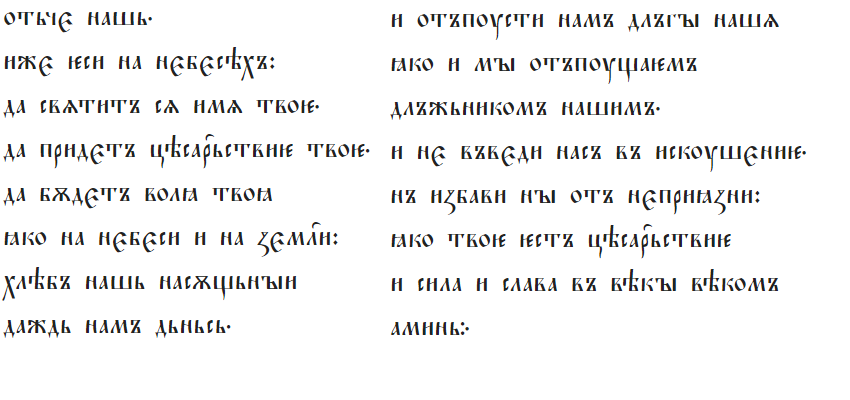
\includegraphics[width=\linewidth]{./sources/of-old-slav.png}
	\caption{Our Father's prayer in Old Slavonic}
	\label{fig:of-old-slav}
\end{figure}

\textbf{Church Slavonic}

Отче наш, Иже еси на небесех!

Да святится имя Твое,

да приидет Царствие Твое,

да будет воля Твоя,

яко на небеси и на земли.

Хлеб наш насущный даждь нам днесь;

и остави нам долги наша,

якоже и мы оставляем должником нашим;

и не введи нас во искушение,

но избави нас от лукаваго.

\begin{figure}
	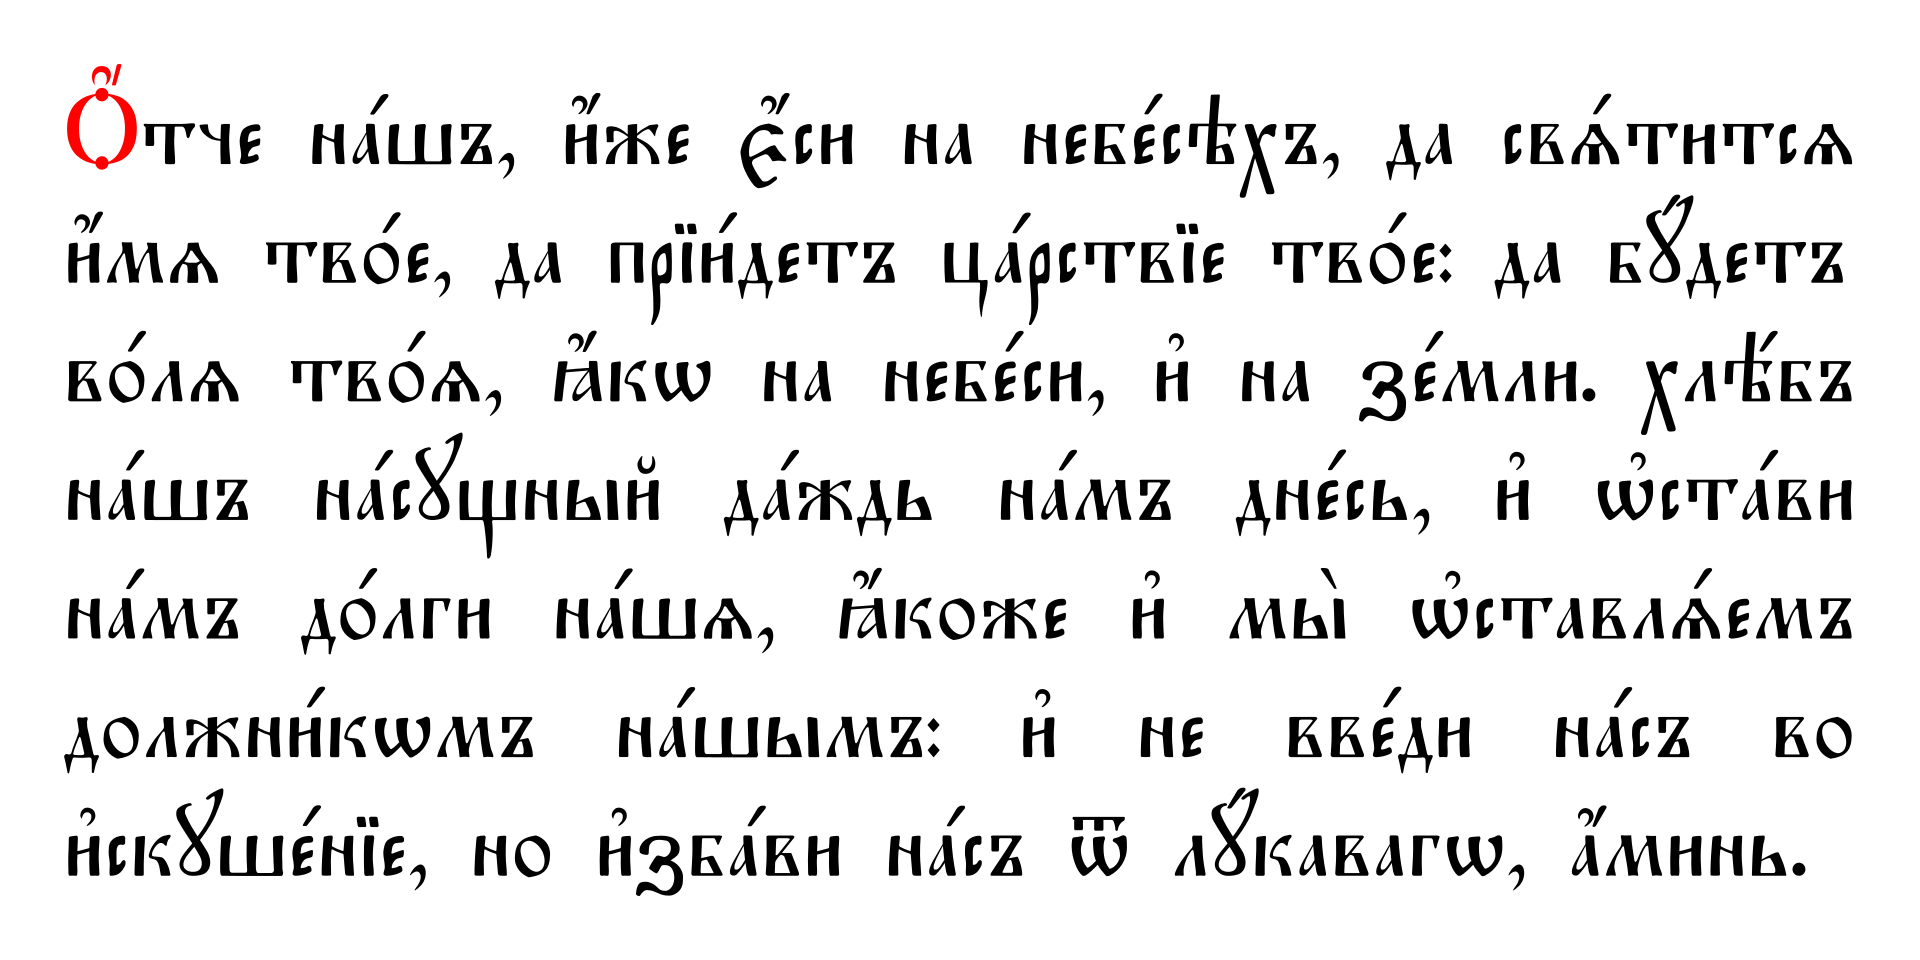
\includegraphics[width=\linewidth]{./sources/of-church-slav.png}
	\caption{Our Father's prayer in Church Slavonic}
	\label{fig:of-church-slav}
\end{figure}

\textbf{Russian}

Отче нашъ, сущій на небесахъ!

да святится имя Твое;

да пріидетъ Царствіе Твое;

да будетъ воля Твоя

и на земл\cyryat, какъ на неб\cyryat;

хл\cyryatбъ нашъ насущный дай намъ на сей день;

и прости намъ долги наши,

какъ и мы прощаемъ должникамъ нашимъ;

и не введи насъ в искушеніе,

но избавь насъ от лукаваго.

\textbf{Belorussian}

Ойча наш,

Які ёсць на нябёсах,

няхай свяціцца імя Тваё,

няхай прыйдзе Царства Тваё,

няхай будзе воля Твая

як на небе, так і на зямлі.

Хлеб наш надзённы дай нам сёння;

і даруй нам даўгі нашы,

як і мы даруем даўжнікам нашым;

і не ўвядзі нас у спакусу,

але збаў нас ад злога. 

\textbf{Belorussian (Tarashkevica)}

Ойча наш, каторы ёсьць на небе! 

Сьвяціся Імя Тваё. 

Прыйдзі Валадарства Тваё. 

Будзь воля Твая 

Як у небе, так і на зямлі. 

Хлеба нашага штодзённага 

дай нам сёньня. 

І адпусьці нам грахі нашы, 

як і мы адпускаем 

вінаватым нашым. 

І ня ўводзь нас у спакусу, 

але збаў нас ад злога. 

\textbf{Ukrainian}

Отче наш, що є в небі,
 
нехай святиться ім'я Твоє.

нехай прийде Царство Твоє,

нехай буде воля Твоя,

як на небі, так і на землі;

Хліба нашого щоденного дай нам сьогодні;

й одпусти нам провини наші,

як і ми відпускаємо винуватцям нашим;

і відведи нас від спокуси,

але визволи нас від злого.

\textbf{Rusyn (Podkarpatsky)}

Отче наш, Котрый ись на небесах!

Най сятить ся имня Твоє;

най прийде Царство Твоє;

най буде воля Твоя,

як на небі так и на земли;

хлiб наш насущный дай нам днесь;

и одпусти нам довгы нашы,

як и мы одпущаєме довжникам нашым;

и не введи нас в искушеніє,

но избав нас од лукавого!

\textbf{Rusyn (Pryashôvsky)}

Отче наш, котрый єсь на небесах,

няй святить ся твоє імя,

няй прийде твоє Царьство,

няй ся дїє твоя воля,

як на небі, так і на земли.

Хлїб наш каждоденный дай нам днесь

і одпусть нам нашы довгы,

так як і мы одпущаме своїм довжникам,

і не приведь нас до покушіня,

но ослободь нас од лукавого.

\textbf{Polish}

Ojcze nasz, któryś jest w niebie,

święć się imię Twoje;

przyjdź królestwo Twoje;

bądź wola Twoja,

jako w niebie tak i na ziemi.

Chleba naszego powszedniego daj nam dzisiaj

i odpuść nam nasze winy,

jako i my odpuszczamy naszym winowajcom.

I nie wódź nas na pokuszenie,

ale nas zbaw ode złego.

\textbf{Kashubian}

Òjcze nasz, jaczi jes w niebie,

niech sã swiãcy Twòje miono,

niech przińdze Twòje królestwò,

niech mdze Twòja wòlô

jakno w niebie tak téż na zemi.

Chleba najégò pòwszédnégò dôj nóm dzysô

i òdpùscë nóm naje winë,

jak i më òdpùszcziwómë naszim winowajcóm.

A nie dopùscë na nas pòkùszeniô,

ale nas zbawi òde złégò.

\textbf{Drawänopolabian}

Nôse Wader,

ta toy gis wa Nebisgáy,

Sjungta woarda Tygí Geima,

Tia Rîk komaj,

Tia Willia śčinyôt,

kok wa Nebisgáy,

tôk kak no Zime.

Nôsi wisedanneisna Stgeiba doy nâm dâns,

un wittedoy nâm nôse Ggrêch,

kak moy wittedoyime nôsem Grêsmarim.

Ni bringoy nôs ka Warśikónye,

tay löśoáy nôs wit wisókak Šaudak.

\textbf{Easter Polabian}

Aita Nos,

tâ toi jis wâ nebesai,

Sjęty wordoj Tyji jaimą,

Tyji Rik komaj,

Tyja wyľa mo są ťyńot,

kok wâ nebesai,

tok no zemi,

nosę wisedanesnę sťaibę doj nam dâns,

a wytâdoj nam nose greche,

kok moi wytâdojeme nosim gresnarem.

Ni bringoj nos wâ Warsykongę,

toi losoj nos wyt wisokag šaudag.

\textbf{Silesian}

Uojcze nasz, keryś je we ńebje

bydź pośwjyncůne mjano Twoje;

przińdź krůlestwo Twoje;

bydź wola Twoja

jako we ńebje tak tyż na źymji;

chlyb nasz kożdodźynny dej nům dźiśo;

a uodpuść nům nasze winy,

jako a my uodpuszczůmy naszym wińńikům;

a ńy wůdź nos na pokuszyńy;

nale zbow nos uode złygo.

\textbf{Upper-Sorbian}

Wótče naš, kiž sy w njebjesach.

Swjeć so Twoje mjeno.

Přińdź Twoje kralestwo.

Stań so Twoja wola,

kaž na njebju, tak na zemi.

Wšědny chlěb naš daj nam dźens.

Wodaj nam naše winy,

jako my tež wodawamy swojim winikam.

A njewjedź nas do spytowanja,

ale wumóž nas wot złeho.

\textbf{Lower-Sorbian}

Wóśce nas, kenž sy na njebju,

wuswěśone buź Twójo mě;

pśiź k nam Twójo kralejstwo;

Twója wóla se stań

ako na njebju, tak teke na zemi.

Wšedny klěb naš daj nam źinsa,

a wódaj nam naše winy,

ako my wódawamy swójim winikam.

A njewjeź nas do spytowanja

ale wumóž nas wót togo złego

\textbf{Czech}

Otče náš, jenž jsi na nebesích,

posvěť se jméno tvé,

přijď království tvé,

buď vůle tvá

jako v nebi, tak i na zemi.

Chléb náš vezdejší dejž nám dnes

a odpusť nám naše viny,

jakož i my odpouštíme našim viníkům

a neuveď nás v pokušení,

ale zbav nás od zlého.

\textbf{Slovak}

Otče náš, ktorý si na nebesiach,

posväť sa meno tvoje,

príď kráľovstvo tvoje,

buď vôľa tvoja ako v nebi, tak i na zemi.

Chlieb náš každodenný daj nám dnes

a odpusť nám naše viny,

ako i my odpúšťame svojim vinníkom,

a neuveď nás do pokušenia,

ale zbav nás Zlého.

\textbf{Slovenian}

Oče naš, ki si v nebesih,

posvečeno bodi tvoje ime,

pridi k nam tvoje kraljestvo,

zgodi se tvoja volja 

kakor v nebesih tako na zemlji.

Daj nam danes naš vsakdanji kruh

in odpusti nam naše dolge,

kakor tudi mi odpuščamo svojim dolžnikom,

in ne vpelji nas v skušnjavo, 

temveč reši nas hudega.

\textbf{Serbian}

Оче наш, који си на небесима,

да се свети име Твоје,

да дође царство Твоје;

да буде воља твоја,

и на земљи као на небу.

Хљеб наш насушни дај нам данас,

и опрости нам дугове наше,

као што и ми опраштамо дужницима својим;

и не уведи нас у искушење,

но избави нас од злога.

\textbf{Croatian}

Oče naš,

koji jesi na nebesima, 

sveti se ime Tvoje, 

dođi kraljevstvo Tvoje, 

budi volja Tvoja, 

kako na nebu, tako i na zemlji.

Kruh naš svagdanji daj nam danas, 

i otpusti nam duge naše, 

kako i mi otpuštamo dužnicima našim, 

i ne uvedi nas u napast, 

nego izbavi nas od Zla!. 

\textbf{Bosnian}

Oče naš,

koji jesi na nebesima,

sveti se ime tvoje,

dođi kraljevstvo tvoje,

budi volja tvoja,

kako na nebu tako i na zemlji.

Kruh naš svagdanji daj nam danas,

i otpusti nama duge naše,

kako i mi otpuštamo dužnicima našim,

i ne uvedi nas u napast,

nego izbavi nas od zla.

\textbf{Macedonian}

Оче наш, кој си на небесата,

да се свети името Твое,

да дојде царството Твое,

да биде волјата Твоја,

како на небото, така и на земјата;

лебот наш насушен дај ни го денес

и прости ни ги долговите наши

како и ние што им ги проштеваме на нашите должници;

и не нè воведувај во искушение,

но избави нè од лукавиот.

\textbf{Bulgarian}

Отче наш, Който си на небесата!

Да се свети Твоето име,

да дойде Твоето Царство,

да бъде Твоята воля,

както на небето, тъй и на земята;

Насъщния ни хляб дай ни днес,

и прости нам дълговете ни,

както и ние прощаваме на нашите длъжници,

и не въведи нас в изкушение,

но избави ни от лукавия;

защото Твое е царството,

и силата, и славата, вовеки веков.

Амин.

\textbf{Romanian}

Tatăl nostru Care ești în ceruri,

sfințească-se numele Tău,

vie împărăția Ta,

fie voia Ta, precum în cer așa și pe Pământ.

Pâinea noastră cea de toate zilele,

dă-ne-o nouă astăzi

și ne iartă nouă greșalele noastre

precum și noi iertăm greșiților noștri

și nu ne duce pe noi în ispită

ci ne izbăvește de cel rău.

\begin{figure}
	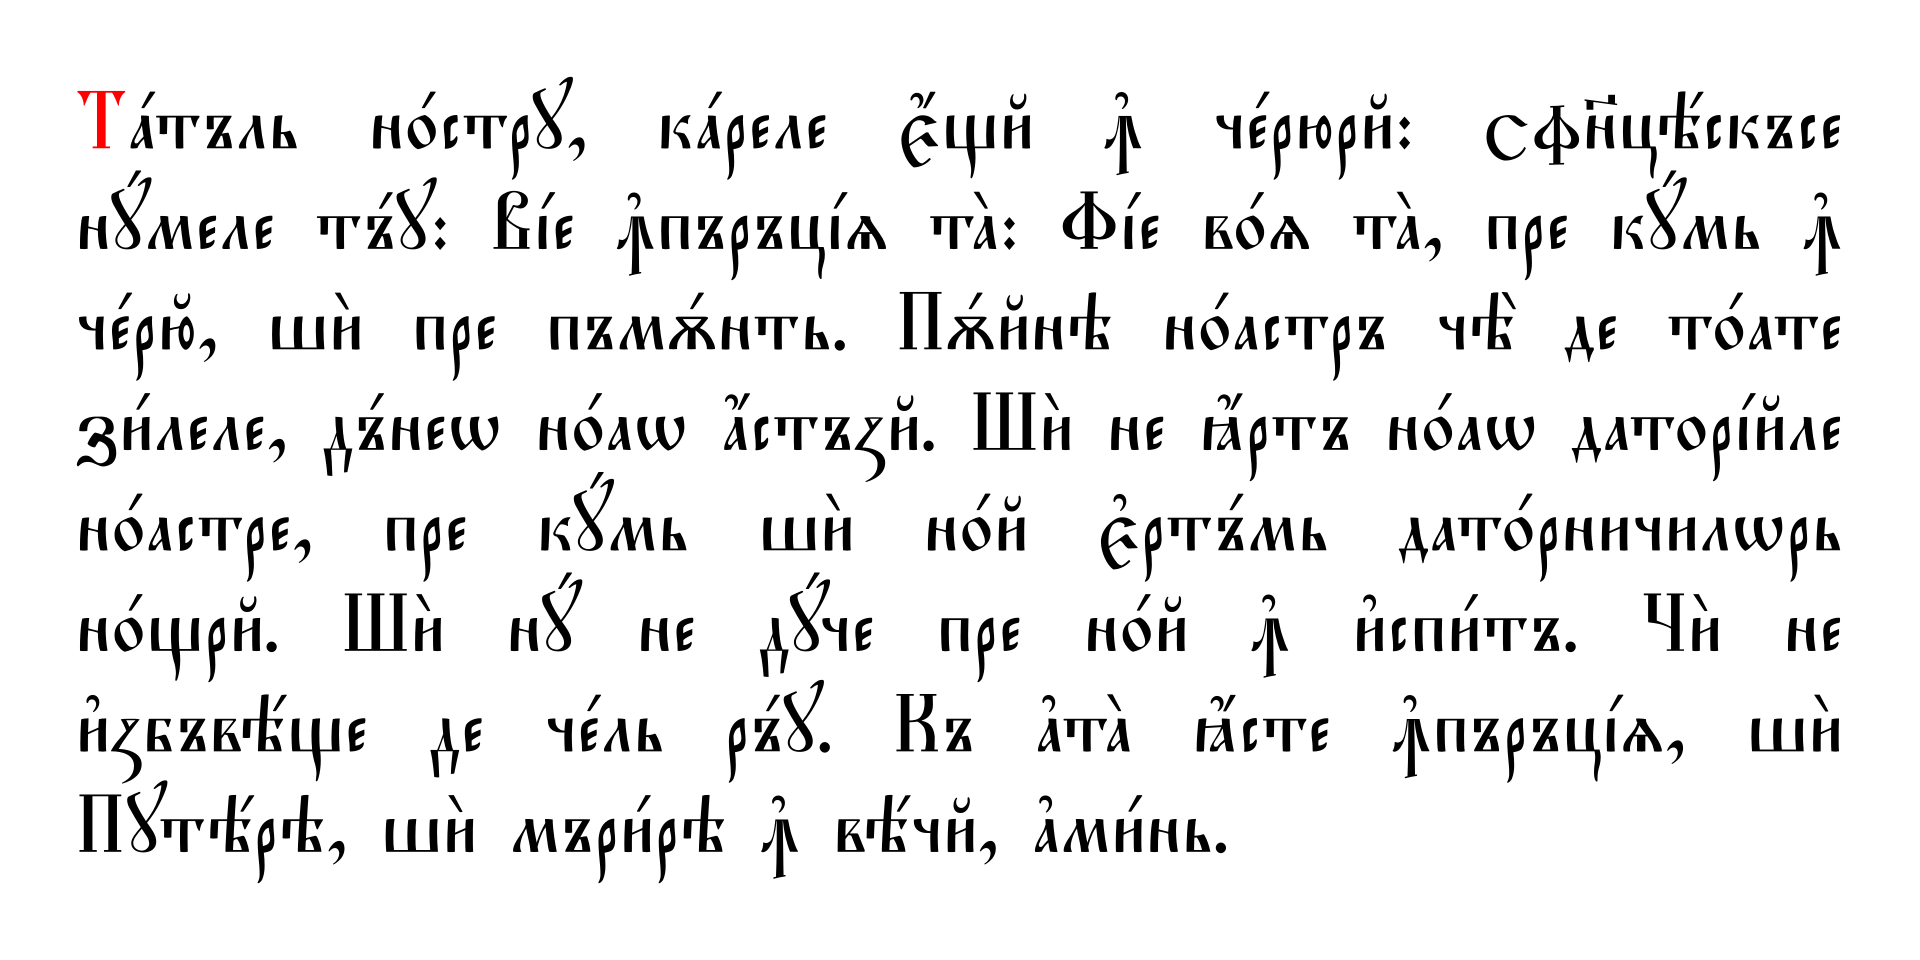
\includegraphics[width=\linewidth]{./sources/of-romanian.png}
	\caption{Our Father's prayer in Romanian}
	\label{fig:of-romanian}
\end{figure}

\textbf{Lithuanian}

Tėve mūsų, kuris esi danguje, 

teesie šventas Tavo vardas,

teateinie Tavo karalystė,

teesie Tavo valia

kaip danguje, taip ir žemėje.

Kasdienės mūsų duonos duok mums šiandien

ir atleisk mums mūsų kaltes,

kaip ir mes atleidžiame savo kaltininkams.

Ir nevesk mūsų į pagundą

bet gelbėk mus nuo pikto.

\textbf{Latvian}

Mūsu Tēvs, debesīs,

Svētīts lai top Tavs vārds.

Lai nāk Tava Valstība.

Tavs prāts lai notiek

kā debesīs, tā arī virs zemes.

Mūsu dienišķo maizi dod mums šodien.

Un piedod mums mūsu parādus,

kā arī mēs piedodam saviem parādniekiem.

Un neieved mūs kārdināšanā,

bet atpestī mūs no ļauna.

\textbf{Latgalian}

Tāvs myusu, kas esi debesīs,

svēteits lai tūp Tovs vōrds.

Lai atnōk Tova vaļsteiba.

Tova vaļa lai nūteik, kai debesīs,

tai ari vērs zemes.

Myusu ikdīneiškū maizi dūd mums šudiņ.

Un atlaid mums myusu porōdus,

kai ari mes atlaižam sovim porōdnīkim.

Un naīved myusu kārdynōšonā,

bet izglōb myusus nu ļauna

\textbf{Old Prussian}

Thawe nuson kas tu asse Andangon,

Swintits wirst twais Emmens;

Pergeis twais Laeims;

Twais Quaits audasseisin na Semmey, key Andangon;

Nusan deininan Geittin deis numons schindeinan;

Bha atwerpeis numans nuson Auschautins, kay mas atwerpimay nuson Auschautenikamans;

Bha ny wedais mans Enperbandan;

Sclait is rankeis mans assa Wargan.
\section{Example texts in Novoslovnica}


\textbf{The agnostic’s prayer}

English original text (R. Zelazny):

Insofar as I may be heard by anything, which may or may not care what I say, I ask, if it matters, that you be forgiven for anything you may have done or failed to do which requires forgiveness. Conversely, if not forgiveness but something else may be required to insure any possible benefit for which you may be eligible after the destruction of your body, I ask that this, whatever it may be, be granted or withheld, as the case may be, in such a manner as to insure your receiving said benefit. I ask this in my capacity as your elected intermediary between yourself and that which may not be yourself, but which may have an interest in the matter of your receiving as much as it is possible for you to receive of this thing, and which may in some way be influenced by this ceremony. Amen.


Novoslovnica translation (tr. by R. Gasparyan):

Ako někto abo něčto može učuti mę i može abo ne može uslyšati mę, če ja bųdu mòlvati, ja prosim, ako prosjba ïmáje značene, dabi byl ty odpušten za če ty byša dělal abo ne dělal i če trěba odpuštati. I ako ne odpuštene, no něčto ïnoje ješto bųde mogati služiti k tvojoǐ poljzě poslě uničtoženä tvojoga těla, ja prosim dabi to něčto ïnoje bilo dano abo ne dano, v odnošenü k slučajam, aby dati ti taku poljzu. Ja prosim to ako tvôǐ posrědnik među tobom i onym, ke može byti ne jesi tobom, no ke ïmáje korystj da ty hte prijęš jak je možno bolëǐ toga ïnoga, če ty možeš prijęti od neĝa, i čto sïǐ obręd može několïko izměniti. Aminj.

\textbf{Litany against fear}

English original text (F. Herbert):

I must not fear.
Fear is the mind-killer.
Fear is the little-death that brings total obliteration.
I will face my fear.
I will permit to pass over me and through me and when it has gone past I will turn the inner eye to see its path.
Where the fear is gone there will be nothing.
Only I will remain. 

Novoslovnica translation (tr. by R. Gasparyan):

Ja ne musim strašiti sę.
Strah je ubiǐcy råzuma.
Strah je malaja smërtj, prinošajučä pòlnoje uničtožene.
Ja bųdu sę větati s mojym strahom oblïka k oblïkě.
Ja hte umožnam sę jemu proǐdati ponad mnoju i skrôz mę, i koĝda on htěše da sę proǐdal, ja bųdu sę smotrati vųtrešnym okom i bųdu sę viděti pųtj ĝo.
Ĝde byše sę proǐdal strah, tamo bųde ničto.
Zôstam sę samo ja.

\textbf{The hymn of Slavs (Hej, Slovania)}

Slovak original text (S. Tomášik):

\begin{verse}
	Hej, Slovania, ešte naša \\
	slovenská reč žije, \\
	Dokiaľ naše verné srdce \\
	za náš národ bije.
	
	Žije, žije, duch slovenský, \\
	bude žiť naveky, \\
	Hrom a peklo, márne vaše \\
	proti nám sú vzteky!
	
	Jazyka dar zveril nám Boh, \\
	Boh náš hromovládny, \\
	Nesmie nám ho teda vyrvať \\
	na tom svete žiadny;
	
	I nechže je koľko ľudí, \\
	toľko čertov v svete; \\
	Boh je s nami: kto proti nám, \\
	toho Parom zmetie.
	
	A nechže sa i nad nami \\
	hrozná búrka vznesie, \\
	Skala puká, dub sa láme \\
	a zem nech sa trasie;
	
	My stojíme stále pevne, \\
	ako múry hradné. \\
	Čierna zem pohltí toho, \\
	kto odstúpi zradne!
\end{verse}

Novoslovnica translation (tr. by G. Carpow):

\begin{verse}
	Geǐ, slověnïe, ješto živo je \\
	Slovo našyh dědov, \\
	Dokųdy odvažno sredco bjije \\
	Našyh slavnyh synov.
	
	Žije, žije duh slověnskyǐ \\
	Živ je toǐ navěkï. \\
	Pěklo je naprasno stalo \\
	Proti nas sëdy.
	
	I podariše jazyk Bôg nam \\
	Našyǐ Bôg-Vlådatelj. \\
	Toǐ je s nami, nikoǐ mogne \\
	Pěsnü našu-ta prestati.
	
	I něhaǐ nad nami búrä \\
	Vznese do něba ŭvysj, \\
	Skala pęka, dųb sę lôma \\
	Zemlötręs tęĝna ŭniz.
	
	Stojeme my tvòrdy, sïlny \\
	Jako stěny gråda \\
	I bųdi proklętym toǐ, ke \\
	Je změnivcom naroda.
\end{verse}

\textbf{Pamętnik sobě sòm zbúdal az netvornyǐ…}

Original text (A.S.Pushkin)

Novoslovnica translation (tr. by G. Carpow)

\begin{verse}
	Pamętnik sobě sòm zbúdal az netvornyǐ, \\
	Ne hte pogyna pųtj dozdě z narodnyh trop. \\	
	Vozstaše vysšeǐ glåvoǐ si on nepokornyǐ \\
	Něž Aleksandriǐskyǐ stòlp.
	
	Ne, cěl ne hte umjram — u žadanomu gudku \\	
	Môǐ tlěn prežive duša, sę sŭobodivša z plït, \\	
	Posláven bųdu az doĝda pod něbom lunnym \\
	Živ bųde jeden hotj pijit.
		
	Posluh o mně prez Rusj hte preǐde vmïg \\	
	I hte nazva mi vsęk jestvučïǐ jazyk v nëǐ \\	
	Slověnov gòrdyǐ ŭnuk, i fïnnov, nyně dïk \\	
	Tunĝus, kalmyk, prijatelj do polëǐ.
	
	I dôlgo bųdu ja prijętnym tym narodu, \\	
	Če gudkom az vozbųđěh dobryh čuǐstv, \\	
	Če v môǐ krut věk vozslávih az sŭobodu, \\	
	Dozovah mïlostj az do mërtvyh duš.
	
	Bože slovo, muzo, čuǐ, bųdi poslušna, \\	
	Ne sę straši ty krivdy, o věncě ty ne dbaǐ, \\	
	Pohvalu ǐ klěvetu priǐmaǐ ty råvnodušno \\	
	I so glupakom ne spëraǐ.
\end{verse}

\textbf{Dvôgovor 1}

— Don’t understand anything: everything is already decided, yet you have not booked the tickets… Do you hope for good luck?

— I’m going only next week. I have eight days left to buy train tickets. If I don’t but them, I’ll go by a bike!

— You’re joking! You can’t go far such a way. I have a brilliant idea: let’s take a taxi!

— I suppose I should not notice that I have no money?

— Come on! If you want to, we’ll go by bus, but we will there in six hours. Look, why don’t you want to go by car?

— I can’t find keys

— Yeah… There’s always something going on with you! I think, we have to look for your car keys.


— Råzumim ničto: vsë je porěšano, ale ty ješto ne si zarezerviral [zakupil] bilěty… Znovu jesi sę zanadějal na uspěh?

— Ja idam samo na slědnoji sedmicji. Zostahu vsï 8 (osem) dnï aby kupiti bilěty na vlåk. Ako ne kupim, hte idam na dvojokolu!

— Ješto žartuješ! Tako ty ne hte idaš dalïko. Imám ĝenijalnu videju: haǐ bëraǐmo taksi!

— Mysläm, že ne trěba pojasnäti, če ne mám pěnęŝëǐ?

— Prestani! Ako tako hteš, hte idama na lüdovozu, ale bųdema jěhati 6 (šest) godin [časov]. Sluhaǐ, a začto ne hteš jěhati na sámovozu?

— Ne mogam najidti klüčëǐ.

— Da… Vsëĝda něčto byvaje s tobom! Mysläm, trěba ješto pošukati klüčï od tvojoga sámovoza.


\textbf{Dvôgovor 2}


— I love holidays! We do nothing, relax, go to a sauna, and our husbands go fishing.

— Yes, it is true, you come home late at night and then still have a dinner to be cooked… And I would like instead of cleaning the nursery and standing by the cooker to read a magazine, to watch TV quietly, or to sit at the bar.

— You work too much: as for me, even out of vacation I go to the cinema, to bars…

— Of course, you don’t have kids yet, and I have a five-year-old son and a grown-up daughter. And you need to work less: your husband can borrow his brand new car, and my husband does not have a car at all.

— That’s also true, but my husband is always saying how I should drive the car: «it is necessary to drive at 60 km / h speed! The car has been parked unsuccessfully!» And nobody tells you how to live.»

— Um… Don’t know what’s better. I have received a drive card, I bought a car on my own, but my husband still laughs at the way I drive.

— Well, I suppose he can express his opinion only in jokes…

— Wow! You are for him!

— Come on, I’m kidding, and you are always getting offended. Let’s just go to the river. At a shallow depth there you can see fish with amazing scales, huge tails and small-small fins.


— Obožam odpusk! Ničto dělame, počivame, hodime do saŭny, a našy mųžy hođut rybovati.

— Da, ïstina, vretaš dodomu z råboty pozdno, poslě trěba ješto večerü gotovati… A htěla bih zaměsto něž čïstiti dětsku komnatu [světlicu] i stojati na kuhnji, to lïstati žurnal, glědati TV ili spokôǐno sidati v báru [kòrčmji].

— Ty dužo mnogo råbotaš: ja hođam v kinemu [kretadlo], v bár [kòrčmu] aǐ ne v odpusku…

— Råzbëra sę, ne máš dětëǐ, az ïmám pętïročinnoga syna i doroslu dčerj. I råbotati trěbaš po-malo: tvôǐ mųž može požičiti ti svôǐ novyǐ sámovoz, a u mojoga ne má.

— To je takođe ïstina, ale mi mųž poslě neustanno govori, čto i kako musim dělati: «Jěhati trěba s bystrostïü 60 km/g! Sámovoz je hudo zaparkovan.» Ami ti nikto govori, kako trěba žiti.

— Hm… Aǐ ne znam, čto je po-dobro. Ja davno ziskah licenzu [vozne pravo], sámovoz kupih sámostatno, ale mųž vsë pako sę směje, kako vodim.

— Z mojoga poglědu, on samo v žartah može izkazati svoje mněne…

— Prošu! Ty si za ĝo!

— Prestani, žartuju, a ty, kako vsëdy, sę obidaš. Něhaǐ idama do rěky. Na malkoji glųbinji je možno uzreti ryb s čuděsnoju šupinoǐ, vëlïkymi hvostami i malymi-malymi plytvami.


\textbf{Dvôgovor 3}


— I heard you got so much makeup for your birthday that you can open a beauty salon!

— What nonsense! Husband made a present: gifted a bit make-up.

— Didn’t you choose it yourself? I’m sure he followed your instructions.

— No, he bought everything himself: I was sick, so I did not even go to the store.

— Damn it! What was wrong with you?

— I don’t know, my stomach hurt, I had diarrhea… maybe it was because of the berries I had eaten before.

— How are you feeling now?

— The pill my doctor had prescribed me started acting very quickly and I felt better. And just in case I’ve drunk paracetamol this morning. I’d rather retire now! I think I’m just working too much.

— You look like mom. She thought about work all the time, too.

— Well, tell me about yourself. You’re going on vacation soon, right?

— Yes, Baikal. I’ve been told so much about him, and as one says, «better to see once than hear a hundred times.»


— Slyšala sòm, že na tvôǐ rođen denj podarihu ti tolïko mnogo kosmetiky až možno odkryti kosmetičnyǐ salon!
— Jaka glupostj! Mųž ztvoriše podarek: nemnogo makijaža.

— Da li ne ty izbëraša vsë? Postoǐna sòm, če on slědovaše tvojim ukazam.

— Ne, on kupiše vsë sámostatno: běh hŭora, tomu daže do tòrgovišta ne pojěhah.

— Preklętno! Čto sę staše s toboǐ?

— Navět ne znam: bolěše brüho, běše diareja [drisk] … Može byti, to z jaĝod, ktoryh ja byh zjědla po-rano.

— A kako jesi nyně?

— Pilulka, ktoru mi byše dal lěkar, započïnaše dějati vëlïmi bystro, i mi staše po-dobro. Za vsęko, dnešnym utrom izpjila sòm paracetamol. Skoro by preǐdti na penzu [dohodku]! Sę kaže mi, če prosto premnogo råbotim.

— Jabelko od jablonï nedalïko pada: jesi kakto svoja materj! Ona takođe vesj čas myslěše o råbotě.

— Dobro, haǐ kaži o sobě. Že skoro jěhaš odpuskovati?

— Da, do Baǐkala. Tolïko mnogo sòm råzkazovahu mi o nem. I kakto sę govori, «Je dobrëǐ jednađy uviditi, něž sto kråt uslyšati’.


\textbf{Dvôgovor 4}


— Dęka ti polųčil sòm dostųp k neograničnomu objimu informacijy.

— Dękuǐ vsëmirnoǐ mrežě, a ne mi: ja sáma znaǐdala sòm ovyǐ saǐt na nějakomu forumu. Samo poslě dovęzanä Mïromrežy, ja stvorih svôǐ bloĝ, de nyně sovětam podobny korystny resursy [zdrojy]. Među tym, môǐ bloĝ je stal dostatočno znanym i pritęga vëlïke množestvo korystnikov vsękoga vozrôsta.

— Ami ja samo dělam pòrvy krocy v Mïromrežji, samo poznal sòm élektronnu poštu. Ujavilo sę, že kromě zvyčaǐnoga teksta prez élektronnu poštu je možno dosylati fotosnïmcy i zvųkovy poslanijy.

— Råzbëra sę, ta ǐ vsęky ïnšy faǐly možno je.

— Ale naprek vygodam od komputera, jestvujut i problemy. Zgorila je moja sistemóva jednota, mál sòm da tęgam ĝo do dělnicy, a on je tęžek.

— Ïmám noŭtbuk. To je po-prosto, v dělnicu ne tako tęžko je da nosiš. Ale jestvujut i mïnusy: něĝda ne mogam naǐdati svôǐ noŭtbuk, a to znači, če môǐ syn gra onlaǐn! Znaš li, če vo mrežji su tako mnogo ïger dlä podrôstkov i ne má sïl ih iztęgati iz Mïromrežy. Ale spravidlóvo trěba da kazam, če vo mrežji on ne samo sę zabavi, no i mnogo rádi.

— Jest sám cěl kakto matj! Vnųtrě dušy niĝda ne sę kolěbah v talentah [darnostäh] tvojyh čęd [dětëǐ].

— Dčeri mi komputery i proĝramovane ne su korystny, ona je DJ. Juž dvě ročiny råboti na radivu, v muzykalnomu predavanü po zakazkam radivosluhatelëǐ.

— Udava že sę lüdäm! Jesòm melomanom [gudbolübom], vsëĝda sòm měčtal stati DJ.

— Može byti, nedocěnovah profesiju-ta, ale z počętku klęh sę, htěh aby ji stati někto drugym, ale nyně råzumim, če ona je pravdivym specijalistom i glědam na ju s odkrytymi okami.

— Dobro je, že ty to si zråzumila, žbo roditelï vsëĝda sę kolěbut v sposobnostäh dětëǐ si.


— Thanks to you, I got access to an unlimited amount of information.

— Thanks to the world wide web, not me: I found this site on some forum. As soon as I was connected to the Internet, I created my blog, where I now advise such interesting resources. By the way, my blog has become quite famous and attracts a huge number of users of all ages.

— And I’m just taking the first steps on the Internet, just opened for myself e-mail. It turned out that in addition to the usual text by e-mail, you can send photos and sound messages.

— Of course, and any other files.

— But despite all the benefits that the computer gives us, there are problems. I burned down the system unit, had to drag it to the workshop, and it is heavy…

— I have a laptop. Of course, it is easier to be carried to workshop. But here are its disadvantages: sometimes I can not find my laptop, which means that my son is playing online! You know, the web has many games for adolescents and you can't drag them off the Internet. In fairness I must say that he is not only playing online, but also a lot of work.

— All mom! Deep down, I never doubted your children’s talents.

— Daughter does not care computers and programming, she’s a DJ! For almost two years she has been working on the radio, in a musical program with requests of radio listeners.

— Lucky people! I myself am a music lover, always dreamed of becoming a DJ.

— Maybe I underestimated this profession, but first I was swearing to myself, I wanted her to become someone else, and now I realize that she is a real specialist, and I look at her with my mouth open.

— It’s great that you understand that, because parents always doubt the abilities of their children.


\textbf{Dvôgovor 5}


— Did you see the ad in today’s paper? Russian company LLC «Trust» is looking for a sales Manager. Their requirements to the candidate: higher education, ability to work both independently and in a team. Solid experience in management and impeccable appearance will be undoubted advantages. Why are you wrinkling your forehead? What are your dislikes?

— You’ve already offered me ten different ads in the last 24 hours, and it feels like you can’t stand me leaving my job.

— What a joke! I don’t care, just thinking about you. A few months ago, someone complained a lot about our boss.…

— When was that? Now everything has changed, we’ve almost become friends. In the new year’s address to the employees, he even congratulated me on the results and gave me a puppy!

— Oh, sweet! He’d rather think about raising your salary. No, seriously, as a colleague to a colleague, you can do better. With your work book, your ability to work and your experience… just imagine: a new job, new adventures, a new life!

— Why do I deserve such care? But maybe you’re right, we should think about it.

— I can’t believe my ears! If you think long you’ll miss a great position. And then the scenario would be: you will understand everything, but it’s too late, you’re whining, start remorse, and then — depression.
— Okay, okay, sure, don’t say such terrible things. After the break I’ll call, it’s noon, there’s probably already all gone for lunch.

— Proper solution. In the meantime, I’ll go talk to our boss. And we need to help him: your place will soon be free, and therefore we need a candidate for this job. I repeat, everything is for you, everything is for you to help: and so, I will be the first candidate…


— Vidila li jesi objavu v dnešnomu denniku? Rusiǐska firma SOO «Trest» šukaje upravitelä prodađ. Ihnï požadavky do kandidata: vysše obrazovane, srųčnostj råbotati sámostoǐno i v družinji. Golěm opyt upravenä i vzornyǐ vid bųdųt okovidnymi plüsami. Začto mòrskaš si lòb? Čto ti ne sę podoba?

— V proběgu poslědnoga dnënočija ty jesi predložil mi desęt råzličnyh objav. Ïmám čuǐstvo, že ty ne možeš da dočękaš, dy ja opustim råbotu si.

— Směšno mi je! Bezråzlično to je, samo o tobě i mysläm. Několïko měsęcov nazad někto ožalil našoga načelnika…

— Pa, koĝda to byše? Nyně vsë je změnilo, my staha praktično kakto prijatelï. V novoročnomu poslanü k slugaram on až pozdråvih mę s rezultatami i podarih mę štenka.

— Ah, kako je mïlo! Pa po-lěpo haǐ pomysli o povyšeně tvojoji poplaty. Ne, seriozno, kako kolega do kolegy — jesi sposobna na po-vëlïke. S trudovoǐ knigoǐ si, s tvojoǐ trųdosposobnostïü i opytom ti… Samo predstavi: nova råbota, nova prigoda, nov život!

— Da načto sòm ziskala taku pěku? Ale, može byti jesi prav, trěba pomyslïti dobro.

— Ne věram na sluh-òt svôǐ! Bųdeš dôlgo dumati, hte propustiš prijimnu dòlžnostj. A dalěǐ bųde tako: vsë hte zråzumiš, ale bųde pozdno, bųdeš kanükati, hte pojavi kajane, a poslě — depresija.

— Dobro, dobro, presvědil si, ne govori vęčë takyh užastëǐ! Poslě prervy hte zatelëfonuju [zaŝvonim], nyně je pôldenj, tamo vsï obědajut, věrojętno.

— Pravidlóvo! A ja dopoĝdy hte idam da govorim s našym načelnikom. Trěba i jemu dopomognuti: město ti skoro hte bųde sŭobodne, a znači trěbame kandidata na vakansiju-ta. Povtoram, vsë dlä vas, vsë aby pomognuti vam vsï: ǐ tako, bųdu pòrvym kandidatom…


\textbf{Dvôgovor 6}

— The country has a crisis, inflation, but the number of billionaires has doubled, as well as horror-and salaries and pensions are ridiculous. And you decided to marry…

— Times change, but there’s still no perfect moment. When you and your mother got married 30 years ago, the climate in the country was even more alarming, the economy was shaken, corruption was terrible. And I got a good job, I have a reliable job, and a lot of good amassed: and I have a house, and a wheelbarrow, and a dacha. Let’s live happily ever after!

— You’re right. And will you go only to the registry office or to the Church too?

— We are sure to go to Church! Not what you were expecting? Despite the fact that she is Orthodox and I am Catholic, we have already agreed on everything. 

Last Sunday we went to the morning service, talked to the priest, received a blessing. We were allowed to get married in the temple, all as it should be.

— Well and good, it’s already time for you to marry, so to speak, to start a new life. And where will the festive feast be organized?

— That’s sick. I want to go to some awesome restaurant, service and live music, and she wants the holiday to be full of old farm, in the village, with traditional music, accordion, balalaika, etc, as well as environmentally friendly products, a real Russian feast, she says. I mean, honestly, it’s kind of freaking me out, but I can’t lose face in front of my future wife. On Saturday we go to watch some old farm with future mother-in-law and father-in-law, whether they were born there, or grew up, but in General it is very dear to them. It is true there are repairs to do, Yes, we still have time. So in the coming months I will work hard at work, and in the evenings on the farm, so that everything is ready for the wedding, as soon as possible. If only forces sufficed, because there is so much work, and I am one…

— Well, I see what you’re getting at.…

— Father, what is it worth, you’re a foreman at the biggest construction site in the city!

— Okay, got it, I’ll send you their builders, one you clearly not cope!


— Ïmáme krizu v dòržava-ta, ïmáme inflaciju, pa samo broǐ milïardarov je sę povysil, a tako hudo — i råbotna plata, i penza sų směšno malě. A vy nahtěla sų da zaženate.

— Doba sę měni, ale idejalnoga momenta ne hte naměrima. Ĝda va s mamoǐ sę ženiha 30 ročin nazad, položenije v dòržavji byše po-nepokôǐnym, ékonomika byše råzložena, korupcija byše strašna. A ja sę ziskah dobro, råbotu mám tvòrdu, ta ǐ vękostj blåg nažil sòm: dom ïmám, vozidlu, vilu [hatku]. Bųdeme žiti zadovôlno!

— Da, jesi pravym. Vy samo do SRCS [Služba registracijy civïlnyh sprav] hte idate ili takođe do còrkvy?

— Obovęzno hte idame do còrkvy! Čto, ne čakal jesi? Navzdor če ona je pravoslávnoju, a jesòm kaŧolikom, my vsë sma dogovorila. V mïnulu nedělü hodihma do jutróvoǐ služby, govorihma s svęštenikom [duhóvnikom], dostiĝala sma blågoslovnostj. Dostala sma zvolene za da sę věnčati [korônovati] v hramu kakto trěba.

— Ta ǐ dobro, vremę juž je da sę ženiš, kako kažut, započïnati nov život. A de bųde svatëbne veselije?

— To je vëlïkyǐ zapyt. Htem v nějakomu dužo dobromu restoranu dabi posluga byla dobra i živa gudba, a ona hte dabi prázdnik byl na nějakomu staromu hutoru, v selištu, s tradiciǐnoju gudboǐ, bajanom, balalaǐkoǐ i td, a takođe ékologično čïstymi produktami pa da s russkym stolovanëm, kako ona kaže.To mi pravdě izvodi iz sebę, ale ne mogam da sę zastydim pred bųdučëǐ ženoǐ. V sųbotu idujema glědati nějak star hutor s bųdučïma tëstëǐ i tëstëm. Da li rodila sų tamo, da li izrostnula, ale ona je mnogo dråga dlä nih. Ïstinskě, tamo trěba dělati remont, ama ïmáme vremę. Tomu, v predny měsęcy hte bųdu råbotati, a věčorom pråcovati na hutoru dabi vsë bylo gotovym k svatjbě. Samo dostati sïl, bo tako mnogo råboty tamo je.

— Pa, viđu, dlä čoga ty govoriš…

— Otče, pa čto ti to stoji, jesi nadzornikom na naǐ-vëlïkoji búdovji vo grådu!

— Dobro, ugovoril jesi mę, hte poslam ti búdóvnikov si, sám ty věrno ne sę spraviš!


\textbf{Dvôgovor 7}


— I’m going on vacation, which is very happy to: so great it is in late February to be in Bali!

— Wow! Where did you buy your ticket, in some Agency?

— No, accidentally on the Internet I found a great offer among the burning tours, paid by credit card and that’s all.

— And we are not going anywhere this winter: there is no money at all. We just finished repairing, and he poured us a pretty penny.

— Why? You had only a kitchen the neighbors flooded to fix as I remember.

— We decided to do everything at once, and to entrust the repair to one familiar architect — Yes, more expensive, but we have not lost. He made us such a bathroom: with a chrome shower column, with hydromassage, made a unique mosaic on the wall.

— Well, then you will spend your vacation in Moscow, walking among the two-meter snowdrifts!

— Laugh… It’s a real nightmare in the streets: neither car can pass nor you. And there are rumors that in one neighboring region there is even more snow than we have. Local authorities are there in a complete panic, trying to avoid the collapse of roofs, but can’t do anything, so people themselves daily clean them from the snow, using saws and shovels.

— This region has always had a fairly low socio-economic level, so I am not surprised that it is there now such a situation.

— Okay, enough about the sad part. Tell me more about what’s on the tour.

— All inclusive: visa, all excursions and meals, and there is an additional 10\% discount, and the hotel — 4 stars! All for nothing!

— How nice! When are you coming?

— We leave on February 29.

— No way.…

— How could that? Look, it’s written here.

— This year February has only 28 days… So here’s the thing: you looked through this tiny line… this tour is for the next year!


— Idu v otpusk, jesòm vëlïmi radym tomu: tako dobro je v koncu sěčnä sę postati na Bali!

— Voŭ! De ty si kupil pųtovane, v nějakoji aĝencijy?

— Ne, slučaǐno najil sòm v Mïromrežji odličnu predlogu među goręčïh pųtovaniǐ, zaplatil sòm kreditnoju kartoǐ i vse.

— A my v zimu-ta nida ne idame: upòlno nemáme pěnęŝëǐ. Samo opravku zakončihu, i byše toǐ vëlïmi drågym.
— Začto? Aǐ vy trěbahu opraviti samo kuhnü, vas, ako pamętam, sôsědy zatopihu.

— My rěšihu razom vsë dělati, a opravläti dati jednomu znajomomu arhitektaru — da, po-drågo, ale my ne sme sę pohybali. On nam stvoriše taku kupalnü: s hromóvoju pròšticoǐ, s vodnym masažom, nepovtorimu ukladnicu [mozaǐku] na stěnji.

— Pa znači, če hte provëdate odpusk v Moskvji, hođačï među dvôhmetróvyh sněgohòlmov.

— Směǐ sę, směǐ sę… Napravdu, užas je na vulicah: ni sámovozom projěhati, ni pehom proǐdati. I kažut, že v sôsidnoji obvlåstji má boljš sněgu, něž u nas. Tųdešna vlåda je v poplohu [panicji], dějut za da izběgat provala strěh, ale ničto mogut zpraviti, tomu lüdi sámy kòždodenno čïstut jih od sněgu, korystačï pïly i lopaty.

— V kraju-òt vsëĝda byše dostj nïzek socijalno-ékonomičnyǐ urovenj, tomu ne sòm zadiven, če tamo je ïsto taka situacija.

— Dobro, dostj o hudom. Lěpš kaži, čto máš objimano v pųtovanü.

— Vsë je objimano: i viza, i vsï proglědky, i jědlo, dodatkóvo tamo je 10\% znïžka i 4-ŝvězdóva gostinica. I vsë to blïzkodarmóvo.

— Kako dobro je! A koĝda vy idate?

— Vylětame 29 sěčnä.

— Ne može byti…

— Kako ne može? Glědaǐ, zdě je napisano.

— V ovoji ročinji je samo 28 dnëǐ… Ta ôt čto to je: ty ne poglědil si ôt na ov mal rędek...To je pųtovane na slědnu ročinu!


\textbf{Dvôgovor 8}


— I couldn’t make up with my husband all week.

— What’s the matter with you?

— I wanted to go to the Tretyakov gallery or to the Garage with a colleague because he is interested in art and especially in painting. Oddly enough that my husband said that he would go with us, but I know that he was neither large nor small museums have never been interesting…

— In my opinion, you exaggerate: remember when we all went to Peterhof together, he liked it very much.

— Of course! He was especially happy when I did not notice one fountain and remained wet to the skin.

— Well, my dear, I remember at the beginning of the week warned you that you should take care of any walks and trips…

— I rather fear your stupid horoscopes, and even your persistence will not bring any results — I will not read them.

— Okay, okay, tell me more about your cultural program at the Museum.

— We went to the «Garage», there was an exhibition of contemporary art and the exhibition of some informal author, who has long been world famous. He impressed me very much: in his paintings one can feel the inner conflict that his predecessors expressed through their works in the 60s. And my husband is pretty loud, at all began to say that it would be a picture written in one day, that even a child could draw… To my horror, the hall was the artist himself, he heard what my husband said and here is started! I’m not one of those who easily panic, but the artist began to shout that my husband does not know what art is, that will ask the organizers of the event to kick him out of the exhibition. Well, all I had to do was throw a tantrum at my husband at home.

— Yeah, you shouldn’t have gone there with your husband.…

— No, I shouldn’t have invited my colleague. If my husband hadn’t been jealous, he would never have gone to the Museum!


— Cělu sedmicu na možěh popraviti odnošene s mųžom.

— Čto sę staše u vas?

— Htěh idati v Tretjakovsku galeriju či v «Ĝaraž» s koleĝom, bo on sę zajima umetstvom, osoblivo malarstvom. Stranno je, ale mųž mi kazal je, če hte ida s nami, ale ja ž znam, če ni maly, ni golěmy muzejy mu niĝda sę podobahu.

— Z mojoga poglědu, ty premnožiš: pamętaš li, koĝda my vsï zajedno hodihme v Petergof, toǐ mu sę vëlïmi byše podobal.

— Razbira sę! Osoblivo mu byše směšno, koĝda ja ne primětih jednoga vodotryska i stah upòlno mokroju.

— Pa, dråga mi, pamętam, že ješto v počętku sedmicy upredih tę, če trěbaš da sę hråniš od vsękyh prohodek i pojězdek.

— Ja boljš bám sę tvojyh glupyh goroskopov, i až upor ti ne donësi nijakyh vyslědkov — ne bųdu čitati jih.

— Dobro, dobro, råzkaži dalëǐ o vašoǐ kuljturnoǐ proĝramě v muzeju.

— Poǐdahme v «Ĝaraž», tamo byše vystavka dnešnoga umetstva i ékspozicija nějakoga neformalnoga tvorca, ktor davno je dostal mïróvu znalostj. On vëlïmi zahvatiše [ïmpresioniraše] mę: v plåtnah ĝo sę čujaš tyǐ vųtrešnyǐ konflikt, čto izražahu prez råboty si poprednicy ĝo. A mųž mi dostj glåsno započïnaše govoriti blïzko vsěh, če biše napisal taku råbotu za jeden denj, če až dětę mogalo biše narisovati ju… K užasu mi v salji-ta byše malar sám, on uslyšaše, če govori mųž mi i… čto sę započïnaše! Ne sòm lěgko panikujema, ale malar staše kričati, če mųž môǐ ne zna, čto je malarstvo i če hte poprosi råzporęditelëǐ vystavky izgnati ĝo s ji. Nu, máh samo histeriku mųžu da započïnam vdomu.

— Da, ne trěbaša idati s mųžom tųda…

— Ne, ne trěbah da zovam tųda koleĝu mi. Ako mųž ne biše žarlëval mę, on niĝda ne poǐdal do muzeja!


\textbf{Dvôgovor 9}


— Oh my God, my vacation turned out to be a quiet horror!

— Why? You were at a friend’s cottage, weren’t you?

— Yeah, but they said they have everything great, but when I arrived, I saw that everything is broken. The tap in the kitchen does not work, the flush is broken, you can not touch the sink, because the pipe is clogged. Said the plumber, but we waited for him for almost a week… They’re so tired of constantly filling your head with nonsense.

— Well, as they say, lovely curse — just gratifying.

— She whines that she needs to go to the gym, that she has cellulite and excess weight, and in the evening eats for five! And he says he wants to leave to the Canary Islands or with friends at the beer festival in Bavaria… No, really, I’m almost not crazy: all sedatives that I was with him, drank. And then there’s air conditioning broke down, breathe — though be hung up.

— You weren’t forced to go to the store?

— No, he went there himself, but every time he forgot the list of products he had to buy. That was wound back on the little things five times a day, bought all sorts of things, and his wife scolded at home, not something bought…

— Well, what have you been doing for so long? You could have gone!

— You know, I am a polite and considerate person: I could not do this to these hospitable and infinitely generous people. Here and suffered their miraculous antics for nearly two months. And when I remember that at home is the wife, smoking is prohibited and the store should be gone to, so immediately the life in the country appears not so bad as it seems…


— Mama mi, odpusk staše mi kakto tïh užas!

— Začto? Byša ž u prijatelëǐ na hatkji, ně li?

— Da, ale oni kazahu, če tamo vsë je super, ale koĝda priǐdah, zabačil, če vsë je polomano. Vodovod na kuhnji ne robi, vodozlïv je zloman, umyvadlo ne može da dotykaš, bo truba je sę zatkala. Kazahu, če byhu zovali vodovodara, ale čękahu je blïzko sedmicy… Tako dokučili su mi: vsëčasno bzduřut.

— Kako sę kaže, mïlency sę psovat samo v slådostj.

— Ona nudi, že trěba idati v sportsalu, če má celülit i prebytečnu tęžinu, a večorom jěda zaměsto pęteryh! A on kaže, če hte v odpusk do Kanar či s prijatelämi na prázdnik pjiva v Bavariju… Ne, pravda, blïzko ošalih s nima: izpih vesj sedativ, če máh s sobom. A tamo ješto klïmatizatar sę sgųbiše, dyšati byše nemožno — hotj sę věšaǐ.

— Ne li tę prinuđahu hoditi do maĝazina [sklada]?

— Ne, on sám hođaše tųda, ale vsęk kråt zabezpamętaše spisek produktov, ktory trěbal da kúpi. Ôt i hođaše dotųde malečno pętïkråtno prez denj, kúpaše něčto bzduru, a žena ĝo vdomu kariše, če byše kúpil čto ne trěba…

— Pa začto tako dôlgo stojaše u nih? Mogaša ujěhati!

— Znaš, jesòm učtivym i taktičnym čelověkom: ne možeh az tako napraviti s tymi gostoprijimnymi i bezgrånično štedrymi lüdima. Ôt i tërpah onyšny podivny vybrycy okolo dvôh měsęcov. Ta ǐ kako vozpamętaš, če vdomu je žena si, dymiti je zabråneno i trěbaš da hodiš do sklada, tak razom život na hatkji postoji ne tako hudym…







% Rodney D. Huddleston, Geoffrey K. Pullum, A Student's Introduction to English Grammar, CUP 2005, p. 183.
% А.А. Кривицкий, А.Е. Михневич, А.И. Подлужный Белорусский язык. Для говорящих по-русски - Минск, Выш. шк., 2008. - 383 с.
% Palmer, F. R., Mood and Modality, Cambridge Univ. Press, 1986 (second edition 2001).


\backmatter
% bibliography, glossary and index would go here.

\end{document}